
    




    
\documentclass[11pt]{article}

    
    \usepackage[breakable]{tcolorbox}
    \tcbset{nobeforeafter} % prevents tcolorboxes being placing in paragraphs
    \usepackage{float}
    \floatplacement{figure}{H} % forces figures to be placed at the correct location
    
    \usepackage[T1]{fontenc}
    % Nicer default font (+ math font) than Computer Modern for most use cases
    \usepackage{mathpazo}

    % Basic figure setup, for now with no caption control since it's done
    % automatically by Pandoc (which extracts ![](path) syntax from Markdown).
    \usepackage{graphicx}
    % We will generate all images so they have a width \maxwidth. This means
    % that they will get their normal width if they fit onto the page, but
    % are scaled down if they would overflow the margins.
    \makeatletter
    \def\maxwidth{\ifdim\Gin@nat@width>\linewidth\linewidth
    \else\Gin@nat@width\fi}
    \makeatother
    \let\Oldincludegraphics\includegraphics
    % Set max figure width to be 80% of text width, for now hardcoded.
    \renewcommand{\includegraphics}[1]{\Oldincludegraphics[width=.8\maxwidth]{#1}}
    % Ensure that by default, figures have no caption (until we provide a
    % proper Figure object with a Caption API and a way to capture that
    % in the conversion process - todo).
    \usepackage{caption}
    \DeclareCaptionLabelFormat{nolabel}{}
    \captionsetup{labelformat=nolabel}

    \usepackage{adjustbox} % Used to constrain images to a maximum size 
    \usepackage{xcolor} % Allow colors to be defined
    \usepackage{enumerate} % Needed for markdown enumerations to work
    \usepackage{geometry} % Used to adjust the document margins
    \usepackage{amsmath} % Equations
    \usepackage{amssymb} % Equations
    \usepackage{textcomp} % defines textquotesingle
    % Hack from http://tex.stackexchange.com/a/47451/13684:
    \AtBeginDocument{%
        \def\PYZsq{\textquotesingle}% Upright quotes in Pygmentized code
    }
    \usepackage{upquote} % Upright quotes for verbatim code
    \usepackage{eurosym} % defines \euro
    \usepackage[mathletters]{ucs} % Extended unicode (utf-8) support
    \usepackage[utf8x]{inputenc} % Allow utf-8 characters in the tex document
    \usepackage{fancyvrb} % verbatim replacement that allows latex
    \usepackage{grffile} % extends the file name processing of package graphics 
                         % to support a larger range 
    % The hyperref package gives us a pdf with properly built
    % internal navigation ('pdf bookmarks' for the table of contents,
    % internal cross-reference links, web links for URLs, etc.)
    \usepackage{hyperref}
    \usepackage{longtable} % longtable support required by pandoc >1.10
    \usepackage{booktabs}  % table support for pandoc > 1.12.2
    \usepackage[inline]{enumitem} % IRkernel/repr support (it uses the enumerate* environment)
    \usepackage[normalem]{ulem} % ulem is needed to support strikethroughs (\sout)
                                % normalem makes italics be italics, not underlines
    \usepackage{mathrsfs}
    

    
    % Colors for the hyperref package
    \definecolor{urlcolor}{rgb}{0,.145,.698}
    \definecolor{linkcolor}{rgb}{.71,0.21,0.01}
    \definecolor{citecolor}{rgb}{.12,.54,.11}

    % ANSI colors
    \definecolor{ansi-black}{HTML}{3E424D}
    \definecolor{ansi-black-intense}{HTML}{282C36}
    \definecolor{ansi-red}{HTML}{E75C58}
    \definecolor{ansi-red-intense}{HTML}{B22B31}
    \definecolor{ansi-green}{HTML}{00A250}
    \definecolor{ansi-green-intense}{HTML}{007427}
    \definecolor{ansi-yellow}{HTML}{DDB62B}
    \definecolor{ansi-yellow-intense}{HTML}{B27D12}
    \definecolor{ansi-blue}{HTML}{208FFB}
    \definecolor{ansi-blue-intense}{HTML}{0065CA}
    \definecolor{ansi-magenta}{HTML}{D160C4}
    \definecolor{ansi-magenta-intense}{HTML}{A03196}
    \definecolor{ansi-cyan}{HTML}{60C6C8}
    \definecolor{ansi-cyan-intense}{HTML}{258F8F}
    \definecolor{ansi-white}{HTML}{C5C1B4}
    \definecolor{ansi-white-intense}{HTML}{A1A6B2}
    \definecolor{ansi-default-inverse-fg}{HTML}{FFFFFF}
    \definecolor{ansi-default-inverse-bg}{HTML}{000000}

    % commands and environments needed by pandoc snippets
    % extracted from the output of `pandoc -s`
    \providecommand{\tightlist}{%
      \setlength{\itemsep}{0pt}\setlength{\parskip}{0pt}}
    \DefineVerbatimEnvironment{Highlighting}{Verbatim}{commandchars=\\\{\}}
    % Add ',fontsize=\small' for more characters per line
    \newenvironment{Shaded}{}{}
    \newcommand{\KeywordTok}[1]{\textcolor[rgb]{0.00,0.44,0.13}{\textbf{{#1}}}}
    \newcommand{\DataTypeTok}[1]{\textcolor[rgb]{0.56,0.13,0.00}{{#1}}}
    \newcommand{\DecValTok}[1]{\textcolor[rgb]{0.25,0.63,0.44}{{#1}}}
    \newcommand{\BaseNTok}[1]{\textcolor[rgb]{0.25,0.63,0.44}{{#1}}}
    \newcommand{\FloatTok}[1]{\textcolor[rgb]{0.25,0.63,0.44}{{#1}}}
    \newcommand{\CharTok}[1]{\textcolor[rgb]{0.25,0.44,0.63}{{#1}}}
    \newcommand{\StringTok}[1]{\textcolor[rgb]{0.25,0.44,0.63}{{#1}}}
    \newcommand{\CommentTok}[1]{\textcolor[rgb]{0.38,0.63,0.69}{\textit{{#1}}}}
    \newcommand{\OtherTok}[1]{\textcolor[rgb]{0.00,0.44,0.13}{{#1}}}
    \newcommand{\AlertTok}[1]{\textcolor[rgb]{1.00,0.00,0.00}{\textbf{{#1}}}}
    \newcommand{\FunctionTok}[1]{\textcolor[rgb]{0.02,0.16,0.49}{{#1}}}
    \newcommand{\RegionMarkerTok}[1]{{#1}}
    \newcommand{\ErrorTok}[1]{\textcolor[rgb]{1.00,0.00,0.00}{\textbf{{#1}}}}
    \newcommand{\NormalTok}[1]{{#1}}
    
    % Additional commands for more recent versions of Pandoc
    \newcommand{\ConstantTok}[1]{\textcolor[rgb]{0.53,0.00,0.00}{{#1}}}
    \newcommand{\SpecialCharTok}[1]{\textcolor[rgb]{0.25,0.44,0.63}{{#1}}}
    \newcommand{\VerbatimStringTok}[1]{\textcolor[rgb]{0.25,0.44,0.63}{{#1}}}
    \newcommand{\SpecialStringTok}[1]{\textcolor[rgb]{0.73,0.40,0.53}{{#1}}}
    \newcommand{\ImportTok}[1]{{#1}}
    \newcommand{\DocumentationTok}[1]{\textcolor[rgb]{0.73,0.13,0.13}{\textit{{#1}}}}
    \newcommand{\AnnotationTok}[1]{\textcolor[rgb]{0.38,0.63,0.69}{\textbf{\textit{{#1}}}}}
    \newcommand{\CommentVarTok}[1]{\textcolor[rgb]{0.38,0.63,0.69}{\textbf{\textit{{#1}}}}}
    \newcommand{\VariableTok}[1]{\textcolor[rgb]{0.10,0.09,0.49}{{#1}}}
    \newcommand{\ControlFlowTok}[1]{\textcolor[rgb]{0.00,0.44,0.13}{\textbf{{#1}}}}
    \newcommand{\OperatorTok}[1]{\textcolor[rgb]{0.40,0.40,0.40}{{#1}}}
    \newcommand{\BuiltInTok}[1]{{#1}}
    \newcommand{\ExtensionTok}[1]{{#1}}
    \newcommand{\PreprocessorTok}[1]{\textcolor[rgb]{0.74,0.48,0.00}{{#1}}}
    \newcommand{\AttributeTok}[1]{\textcolor[rgb]{0.49,0.56,0.16}{{#1}}}
    \newcommand{\InformationTok}[1]{\textcolor[rgb]{0.38,0.63,0.69}{\textbf{\textit{{#1}}}}}
    \newcommand{\WarningTok}[1]{\textcolor[rgb]{0.38,0.63,0.69}{\textbf{\textit{{#1}}}}}
    
    
    % Define a nice break command that doesn't care if a line doesn't already
    % exist.
    \def\br{\hspace*{\fill} \\* }
    % Math Jax compatibility definitions
    \def\gt{>}
    \def\lt{<}
    \let\Oldtex\TeX
    \let\Oldlatex\LaTeX
    \renewcommand{\TeX}{\textrm{\Oldtex}}
    \renewcommand{\LaTeX}{\textrm{\Oldlatex}}
    % Document parameters
    % Document title
    \title{Reimplementation of the published OFC Reservoir Neural Network Model \\
    	Supplementary Materials 1}
    
    
    
    
    
% Pygments definitions
\makeatletter
\def\PY@reset{\let\PY@it=\relax \let\PY@bf=\relax%
    \let\PY@ul=\relax \let\PY@tc=\relax%
    \let\PY@bc=\relax \let\PY@ff=\relax}
\def\PY@tok#1{\csname PY@tok@#1\endcsname}
\def\PY@toks#1+{\ifx\relax#1\empty\else%
    \PY@tok{#1}\expandafter\PY@toks\fi}
\def\PY@do#1{\PY@bc{\PY@tc{\PY@ul{%
    \PY@it{\PY@bf{\PY@ff{#1}}}}}}}
\def\PY#1#2{\PY@reset\PY@toks#1+\relax+\PY@do{#2}}

\expandafter\def\csname PY@tok@w\endcsname{\def\PY@tc##1{\textcolor[rgb]{0.73,0.73,0.73}{##1}}}
\expandafter\def\csname PY@tok@c\endcsname{\let\PY@it=\textit\def\PY@tc##1{\textcolor[rgb]{0.25,0.50,0.50}{##1}}}
\expandafter\def\csname PY@tok@cp\endcsname{\def\PY@tc##1{\textcolor[rgb]{0.74,0.48,0.00}{##1}}}
\expandafter\def\csname PY@tok@k\endcsname{\let\PY@bf=\textbf\def\PY@tc##1{\textcolor[rgb]{0.00,0.50,0.00}{##1}}}
\expandafter\def\csname PY@tok@kp\endcsname{\def\PY@tc##1{\textcolor[rgb]{0.00,0.50,0.00}{##1}}}
\expandafter\def\csname PY@tok@kt\endcsname{\def\PY@tc##1{\textcolor[rgb]{0.69,0.00,0.25}{##1}}}
\expandafter\def\csname PY@tok@o\endcsname{\def\PY@tc##1{\textcolor[rgb]{0.40,0.40,0.40}{##1}}}
\expandafter\def\csname PY@tok@ow\endcsname{\let\PY@bf=\textbf\def\PY@tc##1{\textcolor[rgb]{0.67,0.13,1.00}{##1}}}
\expandafter\def\csname PY@tok@nb\endcsname{\def\PY@tc##1{\textcolor[rgb]{0.00,0.50,0.00}{##1}}}
\expandafter\def\csname PY@tok@nf\endcsname{\def\PY@tc##1{\textcolor[rgb]{0.00,0.00,1.00}{##1}}}
\expandafter\def\csname PY@tok@nc\endcsname{\let\PY@bf=\textbf\def\PY@tc##1{\textcolor[rgb]{0.00,0.00,1.00}{##1}}}
\expandafter\def\csname PY@tok@nn\endcsname{\let\PY@bf=\textbf\def\PY@tc##1{\textcolor[rgb]{0.00,0.00,1.00}{##1}}}
\expandafter\def\csname PY@tok@ne\endcsname{\let\PY@bf=\textbf\def\PY@tc##1{\textcolor[rgb]{0.82,0.25,0.23}{##1}}}
\expandafter\def\csname PY@tok@nv\endcsname{\def\PY@tc##1{\textcolor[rgb]{0.10,0.09,0.49}{##1}}}
\expandafter\def\csname PY@tok@no\endcsname{\def\PY@tc##1{\textcolor[rgb]{0.53,0.00,0.00}{##1}}}
\expandafter\def\csname PY@tok@nl\endcsname{\def\PY@tc##1{\textcolor[rgb]{0.63,0.63,0.00}{##1}}}
\expandafter\def\csname PY@tok@ni\endcsname{\let\PY@bf=\textbf\def\PY@tc##1{\textcolor[rgb]{0.60,0.60,0.60}{##1}}}
\expandafter\def\csname PY@tok@na\endcsname{\def\PY@tc##1{\textcolor[rgb]{0.49,0.56,0.16}{##1}}}
\expandafter\def\csname PY@tok@nt\endcsname{\let\PY@bf=\textbf\def\PY@tc##1{\textcolor[rgb]{0.00,0.50,0.00}{##1}}}
\expandafter\def\csname PY@tok@nd\endcsname{\def\PY@tc##1{\textcolor[rgb]{0.67,0.13,1.00}{##1}}}
\expandafter\def\csname PY@tok@s\endcsname{\def\PY@tc##1{\textcolor[rgb]{0.73,0.13,0.13}{##1}}}
\expandafter\def\csname PY@tok@sd\endcsname{\let\PY@it=\textit\def\PY@tc##1{\textcolor[rgb]{0.73,0.13,0.13}{##1}}}
\expandafter\def\csname PY@tok@si\endcsname{\let\PY@bf=\textbf\def\PY@tc##1{\textcolor[rgb]{0.73,0.40,0.53}{##1}}}
\expandafter\def\csname PY@tok@se\endcsname{\let\PY@bf=\textbf\def\PY@tc##1{\textcolor[rgb]{0.73,0.40,0.13}{##1}}}
\expandafter\def\csname PY@tok@sr\endcsname{\def\PY@tc##1{\textcolor[rgb]{0.73,0.40,0.53}{##1}}}
\expandafter\def\csname PY@tok@ss\endcsname{\def\PY@tc##1{\textcolor[rgb]{0.10,0.09,0.49}{##1}}}
\expandafter\def\csname PY@tok@sx\endcsname{\def\PY@tc##1{\textcolor[rgb]{0.00,0.50,0.00}{##1}}}
\expandafter\def\csname PY@tok@m\endcsname{\def\PY@tc##1{\textcolor[rgb]{0.40,0.40,0.40}{##1}}}
\expandafter\def\csname PY@tok@gh\endcsname{\let\PY@bf=\textbf\def\PY@tc##1{\textcolor[rgb]{0.00,0.00,0.50}{##1}}}
\expandafter\def\csname PY@tok@gu\endcsname{\let\PY@bf=\textbf\def\PY@tc##1{\textcolor[rgb]{0.50,0.00,0.50}{##1}}}
\expandafter\def\csname PY@tok@gd\endcsname{\def\PY@tc##1{\textcolor[rgb]{0.63,0.00,0.00}{##1}}}
\expandafter\def\csname PY@tok@gi\endcsname{\def\PY@tc##1{\textcolor[rgb]{0.00,0.63,0.00}{##1}}}
\expandafter\def\csname PY@tok@gr\endcsname{\def\PY@tc##1{\textcolor[rgb]{1.00,0.00,0.00}{##1}}}
\expandafter\def\csname PY@tok@ge\endcsname{\let\PY@it=\textit}
\expandafter\def\csname PY@tok@gs\endcsname{\let\PY@bf=\textbf}
\expandafter\def\csname PY@tok@gp\endcsname{\let\PY@bf=\textbf\def\PY@tc##1{\textcolor[rgb]{0.00,0.00,0.50}{##1}}}
\expandafter\def\csname PY@tok@go\endcsname{\def\PY@tc##1{\textcolor[rgb]{0.53,0.53,0.53}{##1}}}
\expandafter\def\csname PY@tok@gt\endcsname{\def\PY@tc##1{\textcolor[rgb]{0.00,0.27,0.87}{##1}}}
\expandafter\def\csname PY@tok@err\endcsname{\def\PY@bc##1{\setlength{\fboxsep}{0pt}\fcolorbox[rgb]{1.00,0.00,0.00}{1,1,1}{\strut ##1}}}
\expandafter\def\csname PY@tok@kc\endcsname{\let\PY@bf=\textbf\def\PY@tc##1{\textcolor[rgb]{0.00,0.50,0.00}{##1}}}
\expandafter\def\csname PY@tok@kd\endcsname{\let\PY@bf=\textbf\def\PY@tc##1{\textcolor[rgb]{0.00,0.50,0.00}{##1}}}
\expandafter\def\csname PY@tok@kn\endcsname{\let\PY@bf=\textbf\def\PY@tc##1{\textcolor[rgb]{0.00,0.50,0.00}{##1}}}
\expandafter\def\csname PY@tok@kr\endcsname{\let\PY@bf=\textbf\def\PY@tc##1{\textcolor[rgb]{0.00,0.50,0.00}{##1}}}
\expandafter\def\csname PY@tok@bp\endcsname{\def\PY@tc##1{\textcolor[rgb]{0.00,0.50,0.00}{##1}}}
\expandafter\def\csname PY@tok@fm\endcsname{\def\PY@tc##1{\textcolor[rgb]{0.00,0.00,1.00}{##1}}}
\expandafter\def\csname PY@tok@vc\endcsname{\def\PY@tc##1{\textcolor[rgb]{0.10,0.09,0.49}{##1}}}
\expandafter\def\csname PY@tok@vg\endcsname{\def\PY@tc##1{\textcolor[rgb]{0.10,0.09,0.49}{##1}}}
\expandafter\def\csname PY@tok@vi\endcsname{\def\PY@tc##1{\textcolor[rgb]{0.10,0.09,0.49}{##1}}}
\expandafter\def\csname PY@tok@vm\endcsname{\def\PY@tc##1{\textcolor[rgb]{0.10,0.09,0.49}{##1}}}
\expandafter\def\csname PY@tok@sa\endcsname{\def\PY@tc##1{\textcolor[rgb]{0.73,0.13,0.13}{##1}}}
\expandafter\def\csname PY@tok@sb\endcsname{\def\PY@tc##1{\textcolor[rgb]{0.73,0.13,0.13}{##1}}}
\expandafter\def\csname PY@tok@sc\endcsname{\def\PY@tc##1{\textcolor[rgb]{0.73,0.13,0.13}{##1}}}
\expandafter\def\csname PY@tok@dl\endcsname{\def\PY@tc##1{\textcolor[rgb]{0.73,0.13,0.13}{##1}}}
\expandafter\def\csname PY@tok@s2\endcsname{\def\PY@tc##1{\textcolor[rgb]{0.73,0.13,0.13}{##1}}}
\expandafter\def\csname PY@tok@sh\endcsname{\def\PY@tc##1{\textcolor[rgb]{0.73,0.13,0.13}{##1}}}
\expandafter\def\csname PY@tok@s1\endcsname{\def\PY@tc##1{\textcolor[rgb]{0.73,0.13,0.13}{##1}}}
\expandafter\def\csname PY@tok@mb\endcsname{\def\PY@tc##1{\textcolor[rgb]{0.40,0.40,0.40}{##1}}}
\expandafter\def\csname PY@tok@mf\endcsname{\def\PY@tc##1{\textcolor[rgb]{0.40,0.40,0.40}{##1}}}
\expandafter\def\csname PY@tok@mh\endcsname{\def\PY@tc##1{\textcolor[rgb]{0.40,0.40,0.40}{##1}}}
\expandafter\def\csname PY@tok@mi\endcsname{\def\PY@tc##1{\textcolor[rgb]{0.40,0.40,0.40}{##1}}}
\expandafter\def\csname PY@tok@il\endcsname{\def\PY@tc##1{\textcolor[rgb]{0.40,0.40,0.40}{##1}}}
\expandafter\def\csname PY@tok@mo\endcsname{\def\PY@tc##1{\textcolor[rgb]{0.40,0.40,0.40}{##1}}}
\expandafter\def\csname PY@tok@ch\endcsname{\let\PY@it=\textit\def\PY@tc##1{\textcolor[rgb]{0.25,0.50,0.50}{##1}}}
\expandafter\def\csname PY@tok@cm\endcsname{\let\PY@it=\textit\def\PY@tc##1{\textcolor[rgb]{0.25,0.50,0.50}{##1}}}
\expandafter\def\csname PY@tok@cpf\endcsname{\let\PY@it=\textit\def\PY@tc##1{\textcolor[rgb]{0.25,0.50,0.50}{##1}}}
\expandafter\def\csname PY@tok@c1\endcsname{\let\PY@it=\textit\def\PY@tc##1{\textcolor[rgb]{0.25,0.50,0.50}{##1}}}
\expandafter\def\csname PY@tok@cs\endcsname{\let\PY@it=\textit\def\PY@tc##1{\textcolor[rgb]{0.25,0.50,0.50}{##1}}}

\def\PYZbs{\char`\\}
\def\PYZus{\char`\_}
\def\PYZob{\char`\{}
\def\PYZcb{\char`\}}
\def\PYZca{\char`\^}
\def\PYZam{\char`\&}
\def\PYZlt{\char`\<}
\def\PYZgt{\char`\>}
\def\PYZsh{\char`\#}
\def\PYZpc{\char`\%}
\def\PYZdl{\char`\$}
\def\PYZhy{\char`\-}
\def\PYZsq{\char`\'}
\def\PYZdq{\char`\"}
\def\PYZti{\char`\~}
% for compatibility with earlier versions
\def\PYZat{@}
\def\PYZlb{[}
\def\PYZrb{]}
\makeatother


    % For linebreaks inside Verbatim environment from package fancyvrb. 
    \makeatletter
        \newbox\Wrappedcontinuationbox 
        \newbox\Wrappedvisiblespacebox 
        \newcommand*\Wrappedvisiblespace {\textcolor{red}{\textvisiblespace}} 
        \newcommand*\Wrappedcontinuationsymbol {\textcolor{red}{\llap{\tiny$\m@th\hookrightarrow$}}} 
        \newcommand*\Wrappedcontinuationindent {3ex } 
        \newcommand*\Wrappedafterbreak {\kern\Wrappedcontinuationindent\copy\Wrappedcontinuationbox} 
        % Take advantage of the already applied Pygments mark-up to insert 
        % potential linebreaks for TeX processing. 
        %        {, <, #, %, $, ' and ": go to next line. 
        %        _, }, ^, &, >, - and ~: stay at end of broken line. 
        % Use of \textquotesingle for straight quote. 
        \newcommand*\Wrappedbreaksatspecials {% 
            \def\PYGZus{\discretionary{\char`\_}{\Wrappedafterbreak}{\char`\_}}% 
            \def\PYGZob{\discretionary{}{\Wrappedafterbreak\char`\{}{\char`\{}}% 
            \def\PYGZcb{\discretionary{\char`\}}{\Wrappedafterbreak}{\char`\}}}% 
            \def\PYGZca{\discretionary{\char`\^}{\Wrappedafterbreak}{\char`\^}}% 
            \def\PYGZam{\discretionary{\char`\&}{\Wrappedafterbreak}{\char`\&}}% 
            \def\PYGZlt{\discretionary{}{\Wrappedafterbreak\char`\<}{\char`\<}}% 
            \def\PYGZgt{\discretionary{\char`\>}{\Wrappedafterbreak}{\char`\>}}% 
            \def\PYGZsh{\discretionary{}{\Wrappedafterbreak\char`\#}{\char`\#}}% 
            \def\PYGZpc{\discretionary{}{\Wrappedafterbreak\char`\%}{\char`\%}}% 
            \def\PYGZdl{\discretionary{}{\Wrappedafterbreak\char`\$}{\char`\$}}% 
            \def\PYGZhy{\discretionary{\char`\-}{\Wrappedafterbreak}{\char`\-}}% 
            \def\PYGZsq{\discretionary{}{\Wrappedafterbreak\textquotesingle}{\textquotesingle}}% 
            \def\PYGZdq{\discretionary{}{\Wrappedafterbreak\char`\"}{\char`\"}}% 
            \def\PYGZti{\discretionary{\char`\~}{\Wrappedafterbreak}{\char`\~}}% 
        } 
        % Some characters . , ; ? ! / are not pygmentized. 
        % This macro makes them "active" and they will insert potential linebreaks 
        \newcommand*\Wrappedbreaksatpunct {% 
            \lccode`\~`\.\lowercase{\def~}{\discretionary{\hbox{\char`\.}}{\Wrappedafterbreak}{\hbox{\char`\.}}}% 
            \lccode`\~`\,\lowercase{\def~}{\discretionary{\hbox{\char`\,}}{\Wrappedafterbreak}{\hbox{\char`\,}}}% 
            \lccode`\~`\;\lowercase{\def~}{\discretionary{\hbox{\char`\;}}{\Wrappedafterbreak}{\hbox{\char`\;}}}% 
            \lccode`\~`\:\lowercase{\def~}{\discretionary{\hbox{\char`\:}}{\Wrappedafterbreak}{\hbox{\char`\:}}}% 
            \lccode`\~`\?\lowercase{\def~}{\discretionary{\hbox{\char`\?}}{\Wrappedafterbreak}{\hbox{\char`\?}}}% 
            \lccode`\~`\!\lowercase{\def~}{\discretionary{\hbox{\char`\!}}{\Wrappedafterbreak}{\hbox{\char`\!}}}% 
            \lccode`\~`\/\lowercase{\def~}{\discretionary{\hbox{\char`\/}}{\Wrappedafterbreak}{\hbox{\char`\/}}}% 
            \catcode`\.\active
            \catcode`\,\active 
            \catcode`\;\active
            \catcode`\:\active
            \catcode`\?\active
            \catcode`\!\active
            \catcode`\/\active 
            \lccode`\~`\~ 	
        }
    \makeatother

    \let\OriginalVerbatim=\Verbatim
    \makeatletter
    \renewcommand{\Verbatim}[1][1]{%
        %\parskip\z@skip
        \sbox\Wrappedcontinuationbox {\Wrappedcontinuationsymbol}%
        \sbox\Wrappedvisiblespacebox {\FV@SetupFont\Wrappedvisiblespace}%
        \def\FancyVerbFormatLine ##1{\hsize\linewidth
            \vtop{\raggedright\hyphenpenalty\z@\exhyphenpenalty\z@
                \doublehyphendemerits\z@\finalhyphendemerits\z@
                \strut ##1\strut}%
        }%
        % If the linebreak is at a space, the latter will be displayed as visible
        % space at end of first line, and a continuation symbol starts next line.
        % Stretch/shrink are however usually zero for typewriter font.
        \def\FV@Space {%
            \nobreak\hskip\z@ plus\fontdimen3\font minus\fontdimen4\font
            \discretionary{\copy\Wrappedvisiblespacebox}{\Wrappedafterbreak}
            {\kern\fontdimen2\font}%
        }%
        
        % Allow breaks at special characters using \PYG... macros.
        \Wrappedbreaksatspecials
        % Breaks at punctuation characters . , ; ? ! and / need catcode=\active 	
        \OriginalVerbatim[#1,codes*=\Wrappedbreaksatpunct]%
    }
    \makeatother

    % Exact colors from NB
    \definecolor{incolor}{HTML}{303F9F}
    \definecolor{outcolor}{HTML}{D84315}
    \definecolor{cellborder}{HTML}{CFCFCF}
    \definecolor{cellbackground}{HTML}{F7F7F7}
    
    % prompt
    \newcommand{\prompt}[4]{
        \llap{{\color{#2}[#3]: #4}}\vspace{-1.25em}
    }
    

    
    % Prevent overflowing lines due to hard-to-break entities
    \sloppy 
    % Setup hyperref package
    \hypersetup{
      breaklinks=true,  % so long urls are correctly broken across lines
      colorlinks=true,
      urlcolor=urlcolor,
      linkcolor=linkcolor,
      citecolor=citecolor,
      }
    % Slightly bigger margins than the latex defaults
    
    \geometry{verbose,tmargin=1in,bmargin=1in,lmargin=1in,rmargin=1in}
    
    

    \begin{document}
    
    
    \maketitle
    
    

    
    \hypertarget{python-implementation-of-the-ofc-reservoir-network}{%
\section{Python Implementation of the OFC Reservoir
Network}\label{python-implementation-of-the-ofc-reservoir-network}}

\hypertarget{paradigm-model}{%
\subsection{Paradigm Model}\label{paradigm-model}}

Zhang, et. al.~published in early 2018
\href{https://journals.plos.org/ploscompbiol/article/file?id=10.1371/journal.pcbi.1005925\&type=printable}{A
neural network model for the orbitofrontal cortex and task space
acquisition during reinforcement learning}. Here, the authors
implemented a reservoir neural network whose learning behaviour is
similar to that of mice during all learning phases, including Reversal
Naive and Reversal Expert.

This work takes both inspiration from their work and is motivated by
engineering and biological questions spurred by the model's
implementation and alleged success. I have included the first figure
from their paper which serves as a good overview of their work.

\begin{figure}
\centering
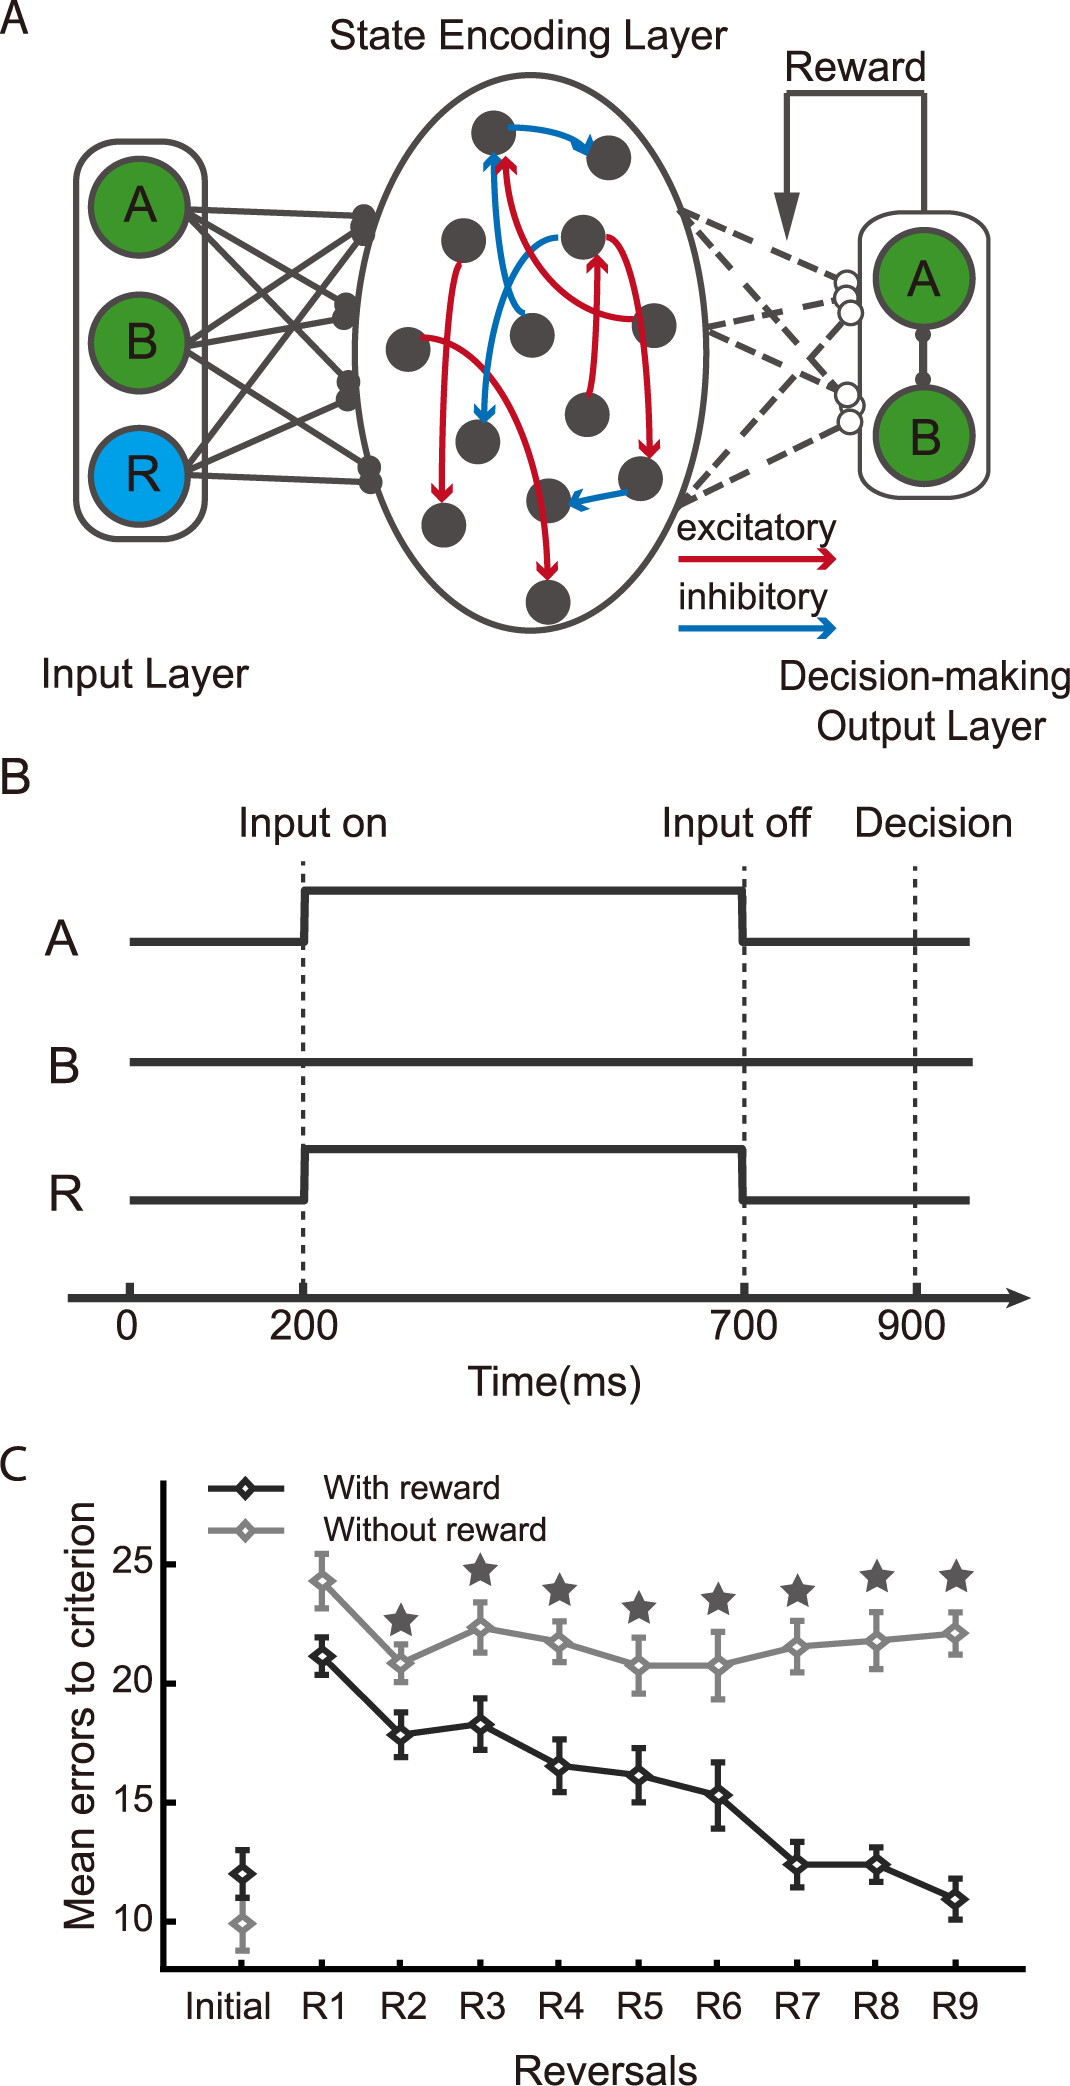
\includegraphics{journal_pcbi_1005925_g001.PNG}
\caption{A diagram of Zhang et. al's reservoir neural network architecture and experimental setup.}
\end{figure}

Their original MATLAB code is also available in the a public
\href{https://github.com/tyangLab/ReservoirNet_OFC_TaskState}{GitHub
repository}.

\hypertarget{mathematics}{%
\subsection{Mathematics}\label{mathematics}}

Below are the mathematical formulations used directly in the reservoir
neural network model. The network has N nodes whose activation value
\(x\) is represented by \begin{align}
\ \tau\frac{dx}{dt}= -x_i + g \sum_{j=1}^N w_{ij} y_j + w_i^{(i)}I + \sigma_{noise}dW_i \\
x(t + 1) = x(t) + \dot{x}(t)\Delta t
\end{align}

Where \(dW_i\) stands for white noise sampled from a uniform
distribution {[}0, 1{]} and \(\sigma_{noise}\) is its variance. \(y_i\)
is the firing rate of neuron \(i\), relative to a \(y_{min}=0\),
\(y_{max}=1\) and baseline firing rate \(y_0 = 0.1\). It is determined
by the following piecewise function: \begin{align}
y=   \left\{
\begin{array}{ll}
      y_0 + y_0 tanh(x/y_0) & x \leq 0   \\
      y_0 + (y_{max} - y_0)*tanh(\frac{x}{y_{max}- y_0}) & x > 0 \\
\end{array} 
\right.
\end{align}

The contributions of each node are then summed to \(v_k\). \(p_k\) then
is determined by performing a softmax on \(v_k\). \(p_k\) then becomes
the expected reward \(E[r_k]\) \begin{align}
v_k = \sum_{i=1}^N w_{out} * y_i \\
p_k = E[r_k] = \frac{e^{-\beta v_k}}{\sum_i e^{-\beta v_i}}
\end{align}

The final output elements \(z_k\) is either 1 with probability \(p_k\)
or 0 with probability \(1 - p_k\) The weighted random choice in this
experiment is between two actions \(a_k\): \(a_1=<0, 1>\) and
\(a_2=<1,0>\), where \(z_1 = 1\) means \(a_1\) was chose, and \(z_2=1\)
means \(a_2\) was chosen.

The weights on the output layer (\(w_{out}\)) are the only ones that are
plastic. These are only updated on the same timestep that the reward
\(r\) is administered because the mice do not receive any information
nor feedback when they refuse to lick, regardless of the texture
presented. The update is relative to the particular decision taken
\(z_k\) and whether a given neuron \(y_i\) had a firing rate greater
than the threshold \(y_{th}\). \begin{align}
\Delta w_{out} = \eta (r - E[r]) (y_i - y_{th}) z_k \\
w_{out}(n + 1) = w_{out}(n) + \Delta w_{out} \\
\end{align} Finally, the weights are normalized after each update:
\begin{align}
w_{out}(n) = \frac{w_{out}(n)}{\sqrt{\sum_{i=1}^N ||w_{out}(n)||^2}}
\end{align}

\hypertarget{implementation}{%
\subsection{Implementation}\label{implementation}}

Below I have directly implemented the formulated model as stated in the
paper and run a few trials using their parameter specifications.

    \begin{tcolorbox}[breakable, size=fbox, boxrule=1pt, pad at break*=1mm,colback=cellbackground, colframe=cellborder]
\prompt{In}{incolor}{1}{\hspace{4pt}}
\begin{Verbatim}[commandchars=\\\{\}]
\PY{c+c1}{\PYZsh{} Imports.}
\PY{o}{\PYZpc{}}\PY{k}{matplotlib} inline
\PY{k+kn}{import} \PY{n+nn}{numpy} \PY{k}{as} \PY{n+nn}{np}
\PY{k+kn}{import} \PY{n+nn}{pandas} \PY{k}{as} \PY{n+nn}{pd}
\PY{k+kn}{import} \PY{n+nn}{matplotlib}\PY{n+nn}{.}\PY{n+nn}{pyplot} \PY{k}{as} \PY{n+nn}{plt}
\PY{k+kn}{from} \PY{n+nn}{matplotlib} \PY{k}{import} \PY{n}{cm}
\PY{k+kn}{from} \PY{n+nn}{matplotlib}\PY{n+nn}{.}\PY{n+nn}{ticker} \PY{k}{import} \PY{n}{LinearLocator}\PY{p}{,} \PY{n}{FormatStrFormatter}
\PY{k+kn}{from} \PY{n+nn}{mpl\PYZus{}toolkits}\PY{n+nn}{.}\PY{n+nn}{mplot3d} \PY{k}{import} \PY{n}{Axes3D}
\PY{k+kn}{import} \PY{n+nn}{matplotlib}\PY{n+nn}{.}\PY{n+nn}{pyplot} \PY{k}{as} \PY{n+nn}{plt}
\PY{k+kn}{from} \PY{n+nn}{scipy}\PY{n+nn}{.}\PY{n+nn}{signal} \PY{k}{import} \PY{n}{butter}\PY{p}{,} \PY{n}{lfilter}\PY{p}{,} \PY{n}{freqz}
\PY{k+kn}{import} \PY{n+nn}{seaborn} \PY{k}{as} \PY{n+nn}{sns}
\PY{n}{sns}\PY{o}{.}\PY{n}{set}\PY{p}{(}\PY{p}{)}
\end{Verbatim}
\end{tcolorbox}

    \begin{tcolorbox}[breakable, size=fbox, boxrule=1pt, pad at break*=1mm,colback=cellbackground, colframe=cellborder]
\prompt{In}{incolor}{2}{\hspace{4pt}}
\begin{Verbatim}[commandchars=\\\{\}]
\PY{c+c1}{\PYZsh{} Experimental parameters.}

\PY{n}{num\PYZus{}trials} \PY{o}{=} \PY{l+m+mi}{1000} \PY{c+c1}{\PYZsh{} Original number: 1000}
\PY{n}{StopTrainingTrials} \PY{o}{=} \PY{l+m+mi}{5000}
\PY{n}{numReversed} \PY{o}{=} \PY{l+m+mi}{100}
\PY{n}{reinforcedSchedule} \PY{o}{=} \PY{l+m+mi}{1} \PY{c+c1}{\PYZsh{} determined or prob}
\PY{n}{withRF} \PY{o}{=} \PY{l+m+mi}{1}  \PY{c+c1}{\PYZsh{} reward feedback}
\PY{n}{numMod} \PY{o}{=} \PY{l+m+mi}{1}
\PY{n}{detail} \PY{o}{=} \PY{l+m+mi}{0}
\PY{n}{REinitial} \PY{o}{=} \PY{l+m+mi}{1}
\PY{n}{simutan}\PY{o}{=} \PY{l+m+mi}{1}
\PY{n}{blocking} \PY{o}{=} \PY{l+m+mi}{0} \PY{c+c1}{\PYZsh{} 0:no block, 1: random block,  2:A block,  3: AR block }

\PY{c+c1}{\PYZsh{} set the time}
\PY{n}{dt} \PY{o}{=} \PY{l+m+mf}{0.001}
\PY{n}{start} \PY{o}{=} \PY{l+m+mf}{0.2}    \PY{c+c1}{\PYZsh{} upon time of stimulus}
\PY{n}{sdur} \PY{o}{=} \PY{l+m+mf}{0.5}    \PY{c+c1}{\PYZsh{} duration of the stimulus}
\PY{n}{inter} \PY{o}{=} \PY{l+m+mi}{0}   \PY{c+c1}{\PYZsh{} interval between stimulus and reward}
\PY{n}{rdur} \PY{o}{=} \PY{l+m+mf}{0.5}    \PY{c+c1}{\PYZsh{} duration of reward input}
\PY{n}{delay} \PY{o}{=} \PY{l+m+mf}{0.2}   \PY{c+c1}{\PYZsh{} delay before decision}
\PY{n}{intertrial} \PY{o}{=} \PY{l+m+mi}{0}
\PY{n}{tau} \PY{o}{=} \PY{l+m+mf}{0.1} \PY{c+c1}{\PYZsh{} time constant }
\end{Verbatim}
\end{tcolorbox}

    \begin{tcolorbox}[breakable, size=fbox, boxrule=1pt, pad at break*=1mm,colback=cellbackground, colframe=cellborder]
\prompt{In}{incolor}{3}{\hspace{4pt}}
\begin{Verbatim}[commandchars=\\\{\}]
\PY{c+c1}{\PYZsh{} Model parameters from OFC paper for the reversal learning task}

\PY{n}{reservoir\PYZus{}network\PYZus{}params} \PY{o}{=} \PY{p}{\PYZob{}}
    \PY{l+s+s1}{\PYZsq{}}\PY{l+s+s1}{tau}\PY{l+s+s1}{\PYZsq{}}         \PY{p}{:} \PY{l+m+mf}{0.1}\PY{p}{,}         \PY{c+c1}{\PYZsh{} 100ms.}
    \PY{l+s+s1}{\PYZsq{}}\PY{l+s+s1}{dt}\PY{l+s+s1}{\PYZsq{}}          \PY{p}{:} \PY{l+m+mf}{0.001}\PY{p}{,}       \PY{c+c1}{\PYZsh{} 1ms.}
    \PY{l+s+s1}{\PYZsq{}}\PY{l+s+s1}{network gain}\PY{l+s+s1}{\PYZsq{}}\PY{p}{:} \PY{l+m+mi}{2}\PY{p}{,}           \PY{c+c1}{\PYZsh{} g}
    \PY{l+s+s1}{\PYZsq{}}\PY{l+s+s1}{training threshold}\PY{l+s+s1}{\PYZsq{}}\PY{p}{:} \PY{l+m+mf}{0.2}\PY{p}{,}   \PY{c+c1}{\PYZsh{} y\PYZus{}th}
    \PY{l+s+s1}{\PYZsq{}}\PY{l+s+s1}{temp parameter}\PY{l+s+s1}{\PYZsq{}}    \PY{p}{:} \PY{l+m+mi}{4}\PY{p}{,}     \PY{c+c1}{\PYZsh{} B (beta)}
    \PY{l+s+s1}{\PYZsq{}}\PY{l+s+s1}{learning rate}\PY{l+s+s1}{\PYZsq{}}     \PY{p}{:} \PY{l+m+mf}{0.001}\PY{p}{,} \PY{c+c1}{\PYZsh{} n (eta)}
    \PY{l+s+s1}{\PYZsq{}}\PY{l+s+s1}{max firing rate}\PY{l+s+s1}{\PYZsq{}}   \PY{p}{:} \PY{l+m+mi}{1}\PY{p}{,}     \PY{c+c1}{\PYZsh{} y\PYZus{}max}
    \PY{l+s+s1}{\PYZsq{}}\PY{l+s+s1}{base firing rate}\PY{l+s+s1}{\PYZsq{}}  \PY{p}{:} \PY{l+m+mf}{0.1}\PY{p}{,}   \PY{c+c1}{\PYZsh{} y\PYZus{}0}
    \PY{l+s+s1}{\PYZsq{}}\PY{l+s+s1}{noise gain}\PY{l+s+s1}{\PYZsq{}}  \PY{p}{:} \PY{l+m+mf}{0.01}\PY{p}{,}        \PY{c+c1}{\PYZsh{} sigma\PYZus{}noise}
    \PY{l+s+s1}{\PYZsq{}}\PY{l+s+s1}{initial noise gain}\PY{l+s+s1}{\PYZsq{}}\PY{p}{:} \PY{l+m+mf}{0.01}\PY{p}{,}  \PY{c+c1}{\PYZsh{} sigma\PYZus{}ini}
    \PY{l+s+s1}{\PYZsq{}}\PY{l+s+s1}{input gain}\PY{l+s+s1}{\PYZsq{}}  \PY{p}{:} \PY{l+m+mi}{4}\PY{p}{,}           \PY{c+c1}{\PYZsh{} g\PYZus{}IR        gain input \PYZhy{}\PYZgt{} reservoir}
    \PY{l+s+s1}{\PYZsq{}}\PY{l+s+s1}{input prob}\PY{l+s+s1}{\PYZsq{}}  \PY{p}{:} \PY{l+m+mf}{0.2}\PY{p}{,}         \PY{c+c1}{\PYZsh{} p\PYZus{}IR        prob input \PYZhy{}\PYZgt{} reservoir}
    \PY{l+s+s1}{\PYZsq{}}\PY{l+s+s1}{hidden layer prob}\PY{l+s+s1}{\PYZsq{}} \PY{p}{:} \PY{l+m+mf}{0.1}\PY{p}{,}   \PY{c+c1}{\PYZsh{} p           Probability of connection in hidden layer}
\PY{p}{\PYZcb{}}
\end{Verbatim}
\end{tcolorbox}

    \begin{tcolorbox}[breakable, size=fbox, boxrule=1pt, pad at break*=1mm,colback=cellbackground, colframe=cellborder]
\prompt{In}{incolor}{4}{\hspace{4pt}}
\begin{Verbatim}[commandchars=\\\{\}]
\PY{c+c1}{\PYZsh{} Helper functions.}

\PY{k}{def} \PY{n+nf}{sigmoid}\PY{p}{(}\PY{n}{x}\PY{p}{,} \PY{n}{x\PYZus{}0}\PY{o}{=}\PY{l+m+mi}{1}\PY{p}{)}\PY{p}{:}
    \PY{k}{return} \PY{l+m+mi}{1}\PY{o}{/}\PY{p}{(}\PY{l+m+mi}{1} \PY{o}{+} \PY{n}{np}\PY{o}{.}\PY{n}{exp}\PY{p}{(}\PY{n}{x}\PY{o}{/}\PY{n}{x\PYZus{}0}\PY{p}{)}\PY{p}{)}

\PY{k}{def} \PY{n+nf}{softmax}\PY{p}{(}\PY{n}{x}\PY{p}{,} \PY{n}{beta}\PY{p}{)}\PY{p}{:}
    \PY{n}{e} \PY{o}{=} \PY{n}{np}\PY{o}{.}\PY{n}{exp}\PY{p}{(}\PY{o}{\PYZhy{}}\PY{n}{beta} \PY{o}{*} \PY{n}{x}\PY{p}{)}
    \PY{k}{return} \PY{n}{e} \PY{o}{/} \PY{n}{e}\PY{o}{.}\PY{n}{sum}\PY{p}{(}\PY{p}{)}
  
\PY{k}{def} \PY{n+nf}{butter\PYZus{}lowpass}\PY{p}{(}\PY{n}{cutoff}\PY{p}{,} \PY{n}{fs}\PY{p}{,} \PY{n}{order}\PY{o}{=}\PY{l+m+mi}{5}\PY{p}{)}\PY{p}{:}
    \PY{n}{nyq} \PY{o}{=} \PY{l+m+mf}{0.5} \PY{o}{*} \PY{n}{fs}
    \PY{n}{normal\PYZus{}cutoff} \PY{o}{=} \PY{n}{cutoff} \PY{o}{/} \PY{n}{nyq}
    \PY{n}{b}\PY{p}{,} \PY{n}{a} \PY{o}{=} \PY{n}{butter}\PY{p}{(}\PY{n}{order}\PY{p}{,} \PY{n}{normal\PYZus{}cutoff}\PY{p}{,} \PY{n}{btype}\PY{o}{=}\PY{l+s+s1}{\PYZsq{}}\PY{l+s+s1}{low}\PY{l+s+s1}{\PYZsq{}}\PY{p}{,} \PY{n}{analog}\PY{o}{=}\PY{k+kc}{False}\PY{p}{)}
    \PY{k}{return} \PY{n}{b}\PY{p}{,} \PY{n}{a}

\PY{k}{def} \PY{n+nf}{butter\PYZus{}lowpass\PYZus{}filter}\PY{p}{(}\PY{n}{data}\PY{p}{,} \PY{n}{cutoff}\PY{p}{,} \PY{n}{fs}\PY{p}{,} \PY{n}{order}\PY{o}{=}\PY{l+m+mi}{5}\PY{p}{)}\PY{p}{:}
    \PY{n}{b}\PY{p}{,} \PY{n}{a} \PY{o}{=} \PY{n}{butter\PYZus{}lowpass}\PY{p}{(}\PY{n}{cutoff}\PY{p}{,} \PY{n}{fs}\PY{p}{,} \PY{n}{order}\PY{o}{=}\PY{n}{order}\PY{p}{)}
    \PY{n}{y} \PY{o}{=} \PY{n}{lfilter}\PY{p}{(}\PY{n}{b}\PY{p}{,} \PY{n}{a}\PY{p}{,} \PY{n}{data}\PY{p}{)}
    \PY{k}{return} \PY{n}{y}
  
\PY{k}{def} \PY{n+nf}{gaussian}\PY{p}{(}\PY{n}{mu}\PY{p}{,}\PY{n}{s2}\PY{p}{)}\PY{p}{:}
    \PY{k}{return} \PY{n}{np}\PY{o}{.}\PY{n}{exp}\PY{p}{(}\PY{o}{\PYZhy{}}\PY{n}{mu}\PY{o}{*}\PY{o}{*}\PY{l+m+mi}{2}\PY{o}{/}\PY{l+m+mi}{2}\PY{o}{/}\PY{n}{s2}\PY{p}{)} \PY{o}{/} \PY{n}{np}\PY{o}{.}\PY{n}{sqrt}\PY{p}{(}\PY{l+m+mi}{2} \PY{o}{*} \PY{n}{np}\PY{o}{.}\PY{n}{pi} \PY{o}{*} \PY{n}{s2}\PY{p}{)}

\PY{k}{def} \PY{n+nf}{smooth}\PY{p}{(}\PY{n}{x1}\PY{p}{,} \PY{n}{x2}\PY{p}{,} \PY{n}{y1}\PY{p}{,} \PY{n}{s2}\PY{p}{)}\PY{p}{:}
    \PY{n}{N2} \PY{o}{=} \PY{n+nb}{len}\PY{p}{(}\PY{n}{x2}\PY{p}{)}
    \PY{n}{y2} \PY{o}{=} \PY{n}{np}\PY{o}{.}\PY{n}{zeros}\PY{p}{(}\PY{n}{N2}\PY{p}{)}

    \PY{c+c1}{\PYZsh{} Check that the new data range does not exceed the old one}
    \PY{n}{rangeX1} \PY{o}{=} \PY{p}{[}\PY{n}{np}\PY{o}{.}\PY{n}{min}\PY{p}{(}\PY{n}{x1}\PY{p}{)}\PY{p}{,} \PY{n}{np}\PY{o}{.}\PY{n}{max}\PY{p}{(}\PY{n}{x1}\PY{p}{)}\PY{p}{]}
    \PY{n}{rangeX2} \PY{o}{=} \PY{p}{[}\PY{n}{np}\PY{o}{.}\PY{n}{min}\PY{p}{(}\PY{n}{x2}\PY{p}{)}\PY{p}{,} \PY{n}{np}\PY{o}{.}\PY{n}{max}\PY{p}{(}\PY{n}{x2}\PY{p}{)}\PY{p}{]}

    \PY{k}{for} \PY{n}{i2} \PY{o+ow}{in} \PY{n+nb}{range}\PY{p}{(}\PY{n}{x2}\PY{o}{.}\PY{n}{size}\PY{p}{)}\PY{p}{:}
        \PY{n}{w\PYZus{}ker} \PY{o}{=} \PY{n}{gaussian}\PY{p}{(}\PY{n}{x2}\PY{p}{[}\PY{n}{i2}\PY{p}{]} \PY{o}{\PYZhy{}} \PY{n}{x1}\PY{p}{,} \PY{n}{s2}\PY{p}{)}
        \PY{n}{w\PYZus{}ker} \PY{o}{/}\PY{o}{=} \PY{n}{np}\PY{o}{.}\PY{n}{sum}\PY{p}{(}\PY{n}{w\PYZus{}ker}\PY{p}{)}
        \PY{n}{y2}\PY{p}{[}\PY{n}{i2}\PY{p}{]} \PY{o}{=} \PY{n}{w\PYZus{}ker}\PY{o}{.}\PY{n}{dot}\PY{p}{(}\PY{n}{y1}\PY{p}{)}

    \PY{k}{return} \PY{n}{y2}
\end{Verbatim}
\end{tcolorbox}

    \begin{tcolorbox}[breakable, size=fbox, boxrule=1pt, pad at break*=1mm,colback=cellbackground, colframe=cellborder]
\prompt{In}{incolor}{5}{\hspace{4pt}}
\begin{Verbatim}[commandchars=\\\{\}]
\PY{c+c1}{\PYZsh{} Implementation of the OFC paper reservoir network.}

\PY{k}{class} \PY{n+nc}{OFCPaperNeuralNetwork}\PY{p}{(}\PY{n+nb}{object}\PY{p}{)}\PY{p}{:}
    \PY{k}{def} \PY{n+nf}{\PYZus{}\PYZus{}init\PYZus{}\PYZus{}}\PY{p}{(}\PY{n+nb+bp}{self}\PY{p}{,} \PY{n}{params}\PY{p}{,} \PY{n}{nodes}\PY{o}{=}\PY{l+m+mi}{500}\PY{p}{,} \PY{n}{input\PYZus{}dim}\PY{o}{=}\PY{l+m+mi}{2}\PY{p}{,} \PY{n}{output\PYZus{}dim}\PY{o}{=}\PY{l+m+mi}{2}\PY{p}{,} \PY{n}{reward\PYZus{}dim}\PY{o}{=}\PY{l+m+mi}{1}\PY{p}{)}\PY{p}{:}
        \PY{n+nb+bp}{self}\PY{o}{.}\PY{n}{output\PYZus{}dim} \PY{o}{=} \PY{n}{output\PYZus{}dim}
        \PY{n+nb+bp}{self}\PY{o}{.}\PY{n}{params} \PY{o}{=} \PY{n}{params}\PY{o}{.}\PY{n}{copy}\PY{p}{(}\PY{p}{)}
        \PY{n+nb+bp}{self}\PY{o}{.}\PY{n}{init\PYZus{}input\PYZus{}weights}\PY{p}{(}\PY{n}{input\PYZus{}dim} \PY{o}{+} \PY{n}{reward\PYZus{}dim}\PY{p}{,} \PY{n}{nodes}\PY{p}{)}
        \PY{n+nb+bp}{self}\PY{o}{.}\PY{n}{init\PYZus{}hidden\PYZus{}weights}\PY{p}{(}\PY{n}{nodes}\PY{p}{)}
        \PY{n+nb+bp}{self}\PY{o}{.}\PY{n}{init\PYZus{}neurons}\PY{p}{(}\PY{n}{nodes}\PY{p}{)}
        \PY{n+nb+bp}{self}\PY{o}{.}\PY{n}{init\PYZus{}output\PYZus{}weights}\PY{p}{(}\PY{n}{nodes}\PY{p}{,} \PY{n}{output\PYZus{}dim}\PY{p}{)}
        \PY{n+nb+bp}{self}\PY{o}{.}\PY{n}{exp\PYZus{}r} \PY{o}{=} \PY{n}{np}\PY{o}{.}\PY{n}{zeros}\PY{p}{(}\PY{n}{output\PYZus{}dim}\PY{p}{)}
        \PY{n+nb+bp}{self}\PY{o}{.}\PY{n}{z} \PY{o}{=} \PY{n}{np}\PY{o}{.}\PY{n}{zeros}\PY{p}{(}\PY{n}{output\PYZus{}dim}\PY{p}{)}

    \PY{k}{def} \PY{n+nf}{init\PYZus{}input\PYZus{}weights}\PY{p}{(}\PY{n+nb+bp}{self}\PY{p}{,} \PY{n}{input\PYZus{}dim}\PY{p}{,} \PY{n}{nodes}\PY{p}{)}\PY{p}{:}
        \PY{n}{std\PYZus{}dev} \PY{o}{=} \PY{n+nb+bp}{self}\PY{o}{.}\PY{n}{params}\PY{p}{[}\PY{l+s+s1}{\PYZsq{}}\PY{l+s+s1}{input gain}\PY{l+s+s1}{\PYZsq{}}\PY{p}{]}  \PY{c+c1}{\PYZsh{} The paper uses a variance of g\PYZus{}IR\PYZca{}2}
        \PY{n}{w\PYZus{}input} \PY{o}{=} \PY{n}{np}\PY{o}{.}\PY{n}{random}\PY{o}{.}\PY{n}{normal}\PY{p}{(}\PY{n}{loc}\PY{o}{=}\PY{l+m+mf}{0.0}\PY{p}{,} \PY{n}{scale}\PY{o}{=}\PY{n}{std\PYZus{}dev}\PY{p}{,} \PY{n}{size}\PY{o}{=}\PY{p}{(}\PY{n}{input\PYZus{}dim}\PY{p}{,} \PY{n}{nodes}\PY{p}{)}\PY{p}{)}
        \PY{n}{p\PYZus{}IR} \PY{o}{=} \PY{n+nb+bp}{self}\PY{o}{.}\PY{n}{params}\PY{p}{[}\PY{l+s+s1}{\PYZsq{}}\PY{l+s+s1}{input prob}\PY{l+s+s1}{\PYZsq{}}\PY{p}{]}
        \PY{n}{indices} \PY{o}{=} \PY{n}{np}\PY{o}{.}\PY{n}{random}\PY{o}{.}\PY{n}{choice}\PY{p}{(}\PY{p}{[}\PY{l+m+mi}{0}\PY{p}{,} \PY{l+m+mi}{1}\PY{p}{]}\PY{p}{,} \PY{n}{size}\PY{o}{=}\PY{n}{w\PYZus{}input}\PY{o}{.}\PY{n}{shape}\PY{p}{,} \PY{n}{p}\PY{o}{=}\PY{p}{[}\PY{l+m+mi}{1} \PY{o}{\PYZhy{}} \PY{n}{p\PYZus{}IR}\PY{p}{,} \PY{n}{p\PYZus{}IR}\PY{p}{]}\PY{p}{)} 
        \PY{n+nb+bp}{self}\PY{o}{.}\PY{n}{w\PYZus{}input} \PY{o}{=} \PY{n}{np}\PY{o}{.}\PY{n}{multiply}\PY{p}{(}\PY{n}{w\PYZus{}input}\PY{p}{,} \PY{n}{indices}\PY{p}{)}

    \PY{k}{def} \PY{n+nf}{init\PYZus{}hidden\PYZus{}weights}\PY{p}{(}\PY{n+nb+bp}{self}\PY{p}{,} \PY{n}{nodes}\PY{p}{)}\PY{p}{:}
        \PY{n}{g} \PY{o}{=} \PY{n+nb+bp}{self}\PY{o}{.}\PY{n}{params}\PY{p}{[}\PY{l+s+s1}{\PYZsq{}}\PY{l+s+s1}{initial noise gain}\PY{l+s+s1}{\PYZsq{}}\PY{p}{]}
        \PY{n}{p} \PY{o}{=} \PY{n+nb+bp}{self}\PY{o}{.}\PY{n}{params}\PY{p}{[}\PY{l+s+s1}{\PYZsq{}}\PY{l+s+s1}{hidden layer prob}\PY{l+s+s1}{\PYZsq{}}\PY{p}{]}
        \PY{n}{std\PYZus{}dev} \PY{o}{=} \PY{n}{g} \PY{o}{/} \PY{n}{np}\PY{o}{.}\PY{n}{sqrt}\PY{p}{(}\PY{n}{p} \PY{o}{*} \PY{n}{nodes}\PY{p}{)} \PY{c+c1}{\PYZsh{} The paper uses a variance of g\PYZca{}2/(p*N)}
        \PY{n}{W} \PY{o}{=} \PY{n}{np}\PY{o}{.}\PY{n}{random}\PY{o}{.}\PY{n}{normal}\PY{p}{(}\PY{n}{loc}\PY{o}{=}\PY{l+m+mf}{0.0}\PY{p}{,} \PY{n}{scale}\PY{o}{=}\PY{n}{std\PYZus{}dev}\PY{p}{,} \PY{n}{size}\PY{o}{=}\PY{p}{(}\PY{n}{nodes}\PY{p}{,} \PY{n}{nodes}\PY{p}{)}\PY{p}{)}
        \PY{n}{indices} \PY{o}{=} \PY{n}{np}\PY{o}{.}\PY{n}{random}\PY{o}{.}\PY{n}{choice}\PY{p}{(}\PY{p}{[}\PY{l+m+mi}{0}\PY{p}{,} \PY{l+m+mi}{1}\PY{p}{]}\PY{p}{,} \PY{n}{size}\PY{o}{=}\PY{n}{W}\PY{o}{.}\PY{n}{shape}\PY{p}{,} \PY{n}{p}\PY{o}{=}\PY{p}{[}\PY{l+m+mi}{1} \PY{o}{\PYZhy{}} \PY{n}{p}\PY{p}{,} \PY{n}{p}\PY{p}{]}\PY{p}{)} 
        \PY{n+nb+bp}{self}\PY{o}{.}\PY{n}{hidden\PYZus{}weights} \PY{o}{=} \PY{n}{np}\PY{o}{.}\PY{n}{multiply}\PY{p}{(}\PY{n}{W}\PY{p}{,} \PY{n}{indices}\PY{p}{)}

    \PY{k}{def} \PY{n+nf}{init\PYZus{}neurons}\PY{p}{(}\PY{n+nb+bp}{self}\PY{p}{,} \PY{n}{nodes}\PY{p}{)}\PY{p}{:}
        \PY{n}{std\PYZus{}dev} \PY{o}{=} \PY{n+nb+bp}{self}\PY{o}{.}\PY{n}{params}\PY{p}{[}\PY{l+s+s1}{\PYZsq{}}\PY{l+s+s1}{initial noise gain}\PY{l+s+s1}{\PYZsq{}}\PY{p}{]} \PY{c+c1}{\PYZsh{} The paper uses a variance of sigma\PYZus{}ini\PYZca{}2}
        \PY{n}{x} \PY{o}{=} \PY{n}{np}\PY{o}{.}\PY{n}{random}\PY{o}{.}\PY{n}{normal}\PY{p}{(}\PY{n}{loc}\PY{o}{=}\PY{l+m+mf}{0.0}\PY{p}{,} \PY{n}{scale}\PY{o}{=}\PY{n}{std\PYZus{}dev}\PY{p}{,} \PY{n}{size}\PY{o}{=}\PY{n}{nodes}\PY{p}{)}
        \PY{n}{y} \PY{o}{=} \PY{n}{np}\PY{o}{.}\PY{n}{ones}\PY{p}{(}\PY{n}{nodes}\PY{p}{)} \PY{o}{*} \PY{n+nb+bp}{self}\PY{o}{.}\PY{n}{params}\PY{p}{[}\PY{l+s+s1}{\PYZsq{}}\PY{l+s+s1}{base firing rate}\PY{l+s+s1}{\PYZsq{}}\PY{p}{]}
        \PY{n+nb+bp}{self}\PY{o}{.}\PY{n}{x} \PY{o}{=} \PY{n}{x}
        \PY{n+nb+bp}{self}\PY{o}{.}\PY{n}{y} \PY{o}{=} \PY{n}{y}

    \PY{k}{def} \PY{n+nf}{init\PYZus{}output\PYZus{}weights}\PY{p}{(}\PY{n+nb+bp}{self}\PY{p}{,} \PY{n}{nodes}\PY{p}{,} \PY{n}{output\PYZus{}dim}\PY{p}{)}\PY{p}{:}
        \PY{n}{W} \PY{o}{=} \PY{n}{np}\PY{o}{.}\PY{n}{random}\PY{o}{.}\PY{n}{normal}\PY{p}{(}\PY{n}{loc}\PY{o}{=}\PY{l+m+mf}{0.0}\PY{p}{,} \PY{n}{scale}\PY{o}{=}\PY{l+m+mi}{1}\PY{p}{,} \PY{n}{size}\PY{o}{=}\PY{p}{(}\PY{n}{nodes}\PY{p}{,} \PY{n}{output\PYZus{}dim}\PY{p}{)}\PY{p}{)}
        \PY{c+c1}{\PYZsh{} According to the paper: normalize according to the squared sum of the weights for each output node.}
        \PY{n}{W} \PY{o}{=} \PY{n}{W}\PY{o}{/}\PY{n}{np}\PY{o}{.}\PY{n}{sqrt}\PY{p}{(}\PY{n}{np}\PY{o}{.}\PY{n}{square}\PY{p}{(}\PY{n}{W}\PY{p}{)}\PY{o}{.}\PY{n}{sum}\PY{p}{(}\PY{n}{axis}\PY{o}{=}\PY{l+m+mi}{0}\PY{p}{)}\PY{p}{)}
        \PY{n+nb+bp}{self}\PY{o}{.}\PY{n}{output\PYZus{}weights} \PY{o}{=} \PY{n}{W}
    
    \PY{k}{def} \PY{n+nf}{step}\PY{p}{(}\PY{n+nb+bp}{self}\PY{p}{,} \PY{n}{I}\PY{o}{=}\PY{l+m+mi}{0}\PY{p}{)}\PY{p}{:}
        \PY{k}{if} \PY{n}{np}\PY{o}{.}\PY{n}{array\PYZus{}equal}\PY{p}{(}\PY{n}{I}\PY{p}{,} \PY{l+m+mi}{0}\PY{p}{)}\PY{p}{:}
            \PY{n}{I} \PY{o}{=} \PY{n}{np}\PY{o}{.}\PY{n}{zeros}\PY{p}{(}\PY{n+nb+bp}{self}\PY{o}{.}\PY{n}{w\PYZus{}input}\PY{o}{.}\PY{n}{shape}\PY{p}{[}\PY{l+m+mi}{0}\PY{p}{]}\PY{p}{)}

        \PY{n}{tau} \PY{o}{=} \PY{n+nb+bp}{self}\PY{o}{.}\PY{n}{params}\PY{p}{[}\PY{l+s+s1}{\PYZsq{}}\PY{l+s+s1}{tau}\PY{l+s+s1}{\PYZsq{}}\PY{p}{]}
        \PY{n}{dt} \PY{o}{=} \PY{n+nb+bp}{self}\PY{o}{.}\PY{n}{params}\PY{p}{[}\PY{l+s+s1}{\PYZsq{}}\PY{l+s+s1}{dt}\PY{l+s+s1}{\PYZsq{}}\PY{p}{]}
        \PY{n}{g} \PY{o}{=} \PY{n+nb+bp}{self}\PY{o}{.}\PY{n}{params}\PY{p}{[}\PY{l+s+s1}{\PYZsq{}}\PY{l+s+s1}{network gain}\PY{l+s+s1}{\PYZsq{}}\PY{p}{]}
        \PY{n}{sigma\PYZus{}noise} \PY{o}{=} \PY{n+nb+bp}{self}\PY{o}{.}\PY{n}{params}\PY{p}{[}\PY{l+s+s1}{\PYZsq{}}\PY{l+s+s1}{noise gain}\PY{l+s+s1}{\PYZsq{}}\PY{p}{]}
        \PY{n}{y\PYZus{}0} \PY{o}{=} \PY{n+nb+bp}{self}\PY{o}{.}\PY{n}{params}\PY{p}{[}\PY{l+s+s1}{\PYZsq{}}\PY{l+s+s1}{base firing rate}\PY{l+s+s1}{\PYZsq{}}\PY{p}{]}
        \PY{n}{y\PYZus{}max} \PY{o}{=} \PY{n+nb+bp}{self}\PY{o}{.}\PY{n}{params}\PY{p}{[}\PY{l+s+s1}{\PYZsq{}}\PY{l+s+s1}{max firing rate}\PY{l+s+s1}{\PYZsq{}}\PY{p}{]}
        
        \PY{n}{white\PYZus{}noise} \PY{o}{=} \PY{n}{np}\PY{o}{.}\PY{n}{random}\PY{o}{.}\PY{n}{randint}\PY{p}{(}\PY{l+m+mi}{0}\PY{p}{,} \PY{n}{high}\PY{o}{=}\PY{p}{(}\PY{l+m+mi}{1} \PY{o}{+} \PY{l+m+mi}{1}\PY{p}{)}\PY{p}{,} \PY{n}{size}\PY{o}{=}\PY{n+nb+bp}{self}\PY{o}{.}\PY{n}{x}\PY{o}{.}\PY{n}{size}\PY{p}{)}
        
        \PY{n}{dx\PYZus{}dt} \PY{o}{=} \PY{l+m+mi}{1}\PY{o}{/}\PY{n}{tau} \PY{o}{*} \PY{p}{(}\PY{o}{\PYZhy{}}\PY{n+nb+bp}{self}\PY{o}{.}\PY{n}{x} \PY{o}{+} \PY{n}{g} \PY{o}{*} \PY{n}{np}\PY{o}{.}\PY{n}{dot}\PY{p}{(}\PY{n+nb+bp}{self}\PY{o}{.}\PY{n}{hidden\PYZus{}weights}\PY{p}{,} \PY{n+nb+bp}{self}\PY{o}{.}\PY{n}{y}\PY{p}{)} 
                         \PY{o}{+} \PY{n}{np}\PY{o}{.}\PY{n}{dot}\PY{p}{(}\PY{n+nb+bp}{self}\PY{o}{.}\PY{n}{w\PYZus{}input}\PY{o}{.}\PY{n}{T}\PY{p}{,} \PY{n}{I}\PY{p}{)} 
                         \PY{o}{+} \PY{n}{sigma\PYZus{}noise} \PY{o}{*} \PY{n}{white\PYZus{}noise}\PY{p}{)}
        \PY{n+nb+bp}{self}\PY{o}{.}\PY{n}{x} \PY{o}{+}\PY{o}{=} \PY{n}{dx\PYZus{}dt} \PY{o}{*} \PY{n}{dt}
        
        \PY{n}{y\PYZus{}conditions} \PY{o}{=}\PY{p}{[}\PY{n+nb+bp}{self}\PY{o}{.}\PY{n}{x} \PY{o}{\PYZlt{}}\PY{o}{=} \PY{l+m+mi}{0}\PY{p}{,} \PY{n+nb+bp}{self}\PY{o}{.}\PY{n}{x} \PY{o}{\PYZgt{}} \PY{l+m+mi}{0}\PY{p}{]}
        \PY{n}{y\PYZus{}functions} \PY{o}{=}\PY{p}{[}
            \PY{k}{lambda} \PY{n}{x}\PY{p}{:} \PY{n}{y\PYZus{}0} \PY{o}{+} \PY{n}{y\PYZus{}0} \PY{o}{*} \PY{n}{np}\PY{o}{.}\PY{n}{tanh}\PY{p}{(}\PY{n}{x}\PY{o}{/}\PY{n}{y\PYZus{}0}\PY{p}{)}\PY{p}{,}
            \PY{k}{lambda} \PY{n}{x}\PY{p}{:} \PY{n}{y\PYZus{}0} \PY{o}{+} \PY{p}{(}\PY{n}{y\PYZus{}max} \PY{o}{\PYZhy{}} \PY{n}{y\PYZus{}0}\PY{p}{)} \PY{o}{*} \PY{n}{np}\PY{o}{.}\PY{n}{tanh}\PY{p}{(}\PY{n}{x}\PY{o}{/}\PY{p}{(}\PY{n}{y\PYZus{}max} \PY{o}{\PYZhy{}} \PY{n}{y\PYZus{}0}\PY{p}{)}\PY{p}{)}
        \PY{p}{]}
        \PY{n+nb+bp}{self}\PY{o}{.}\PY{n}{y} \PY{o}{=} \PY{n}{np}\PY{o}{.}\PY{n}{piecewise}\PY{p}{(}\PY{n+nb+bp}{self}\PY{o}{.}\PY{n}{x}\PY{p}{,} \PY{n}{y\PYZus{}conditions}\PY{p}{,} \PY{n}{y\PYZus{}functions}\PY{p}{)}
        
        \PY{n}{v\PYZus{}k} \PY{o}{=} \PY{n}{np}\PY{o}{.}\PY{n}{dot}\PY{p}{(}\PY{n+nb+bp}{self}\PY{o}{.}\PY{n}{y}\PY{p}{,} \PY{n+nb+bp}{self}\PY{o}{.}\PY{n}{output\PYZus{}weights}\PY{p}{)}
        \PY{n}{beta} \PY{o}{=} \PY{n+nb+bp}{self}\PY{o}{.}\PY{n}{params}\PY{p}{[}\PY{l+s+s1}{\PYZsq{}}\PY{l+s+s1}{temp parameter}\PY{l+s+s1}{\PYZsq{}}\PY{p}{]}
        \PY{n}{p\PYZus{}k} \PY{o}{=} \PY{n}{softmax}\PY{p}{(}\PY{n}{v\PYZus{}k}\PY{p}{,} \PY{n}{beta}\PY{p}{)}
        
        \PY{c+c1}{\PYZsh{}self.z = np.greater\PYZus{}equal(p\PYZus{}k, p\PYZus{}k.max()).astype(float)}
        \PY{n}{choice\PYZus{}idx} \PY{o}{=} \PY{n}{np}\PY{o}{.}\PY{n}{random}\PY{o}{.}\PY{n}{choice}\PY{p}{(}\PY{n}{p\PYZus{}k}\PY{o}{.}\PY{n}{shape}\PY{p}{[}\PY{l+m+mi}{0}\PY{p}{]}\PY{p}{,} \PY{n}{p}\PY{o}{=}\PY{n}{p\PYZus{}k}\PY{p}{)}
        \PY{n+nb+bp}{self}\PY{o}{.}\PY{n}{z} \PY{o}{=} \PY{n}{np}\PY{o}{.}\PY{n}{zeros}\PY{p}{(}\PY{n}{p\PYZus{}k}\PY{o}{.}\PY{n}{shape}\PY{p}{)}
        \PY{n+nb+bp}{self}\PY{o}{.}\PY{n}{z}\PY{p}{[}\PY{n}{choice\PYZus{}idx}\PY{p}{]} \PY{o}{=} \PY{l+m+mi}{1}
         
            
        \PY{n+nb+bp}{self}\PY{o}{.}\PY{n}{exp\PYZus{}r} \PY{o}{=} \PY{n}{p\PYZus{}k}
        \PY{k}{return} \PY{n+nb+bp}{self}\PY{o}{.}\PY{n}{z}

    \PY{k}{def} \PY{n+nf}{receive\PYZus{}reward}\PY{p}{(}\PY{n+nb+bp}{self}\PY{p}{,} \PY{n}{r}\PY{p}{)}\PY{p}{:}
        \PY{n+nb+bp}{self}\PY{o}{.}\PY{n}{update\PYZus{}weights}\PY{p}{(}\PY{n}{r}\PY{p}{)}

    \PY{k}{def} \PY{n+nf}{update\PYZus{}weights}\PY{p}{(}\PY{n+nb+bp}{self}\PY{p}{,} \PY{n}{r}\PY{p}{)}\PY{p}{:}
        \PY{n}{row\PYZus{}vec} \PY{o}{=} \PY{n+nb+bp}{self}\PY{o}{.}\PY{n}{y} \PY{o}{\PYZhy{}} \PY{n+nb+bp}{self}\PY{o}{.}\PY{n}{params}\PY{p}{[}\PY{l+s+s1}{\PYZsq{}}\PY{l+s+s1}{training threshold}\PY{l+s+s1}{\PYZsq{}}\PY{p}{]}
        \PY{n}{col\PYZus{}vec} \PY{o}{=} \PY{n}{np}\PY{o}{.}\PY{n}{multiply}\PY{p}{(}\PY{p}{(}\PY{n}{r} \PY{o}{\PYZhy{}} \PY{n+nb+bp}{self}\PY{o}{.}\PY{n}{exp\PYZus{}r}\PY{p}{)}\PY{p}{,} \PY{n+nb+bp}{self}\PY{o}{.}\PY{n}{z}\PY{p}{)}
        \PY{n}{delta\PYZus{}w} \PY{o}{=} \PY{n+nb+bp}{self}\PY{o}{.}\PY{n}{params}\PY{p}{[}\PY{l+s+s1}{\PYZsq{}}\PY{l+s+s1}{learning rate}\PY{l+s+s1}{\PYZsq{}}\PY{p}{]} \PY{o}{*} \PY{n}{np}\PY{o}{.}\PY{n}{outer}\PY{p}{(}\PY{n}{row\PYZus{}vec}\PY{p}{,} \PY{n}{col\PYZus{}vec}\PY{p}{)}
        \PY{n+nb+bp}{self}\PY{o}{.}\PY{n}{output\PYZus{}weights} \PY{o}{+}\PY{o}{=} \PY{n}{delta\PYZus{}w}
          
\PY{c+c1}{\PYZsh{}         delta\PYZus{}w = self.params[\PYZsq{}learning rate\PYZsq{}] * np.outer((r \PYZhy{} self.exp\PYZus{}r),}
\PY{c+c1}{\PYZsh{}           (self.y \PYZhy{} self.params[\PYZsq{}training threshold\PYZsq{}]))}
\PY{c+c1}{\PYZsh{}         delta\PYZus{}w = np.multiply(delta\PYZus{}w.T, self.z)}
\PY{c+c1}{\PYZsh{}         self.output\PYZus{}weights += delta\PYZus{}w}

        \PY{c+c1}{\PYZsh{} Normalize weights}
        \PY{n+nb+bp}{self}\PY{o}{.}\PY{n}{output\PYZus{}weights} \PY{o}{/}\PY{o}{=} \PY{n}{np}\PY{o}{.}\PY{n}{linalg}\PY{o}{.}\PY{n}{norm}\PY{p}{(}\PY{n+nb+bp}{self}\PY{o}{.}\PY{n}{output\PYZus{}weights}\PY{p}{)}

    \PY{k}{def} \PY{n+nf}{get\PYZus{}output}\PY{p}{(}\PY{n+nb+bp}{self}\PY{p}{,} \PY{n}{exp}\PY{o}{=}\PY{k+kc}{False}\PY{p}{)}\PY{p}{:}
        \PY{k}{if} \PY{n}{exp}\PY{p}{:}
            \PY{k}{return} \PY{n+nb+bp}{self}\PY{o}{.}\PY{n}{z}\PY{p}{,} \PY{n+nb+bp}{self}\PY{o}{.}\PY{n}{exp\PYZus{}r}
        \PY{k}{else}\PY{p}{:}
            \PY{k}{return} \PY{n+nb+bp}{self}\PY{o}{.}\PY{n}{z}
\end{Verbatim}
\end{tcolorbox}

    \begin{tcolorbox}[breakable, size=fbox, boxrule=1pt, pad at break*=1mm,colback=cellbackground, colframe=cellborder]
\prompt{In}{incolor}{6}{\hspace{4pt}}
\begin{Verbatim}[commandchars=\\\{\}]
\PY{c+c1}{\PYZsh{} Experiment function.}

\PY{k}{def} \PY{n+nf}{simple\PYZus{}experiment}\PY{p}{(}\PY{n}{I}\PY{p}{,} \PY{n}{T}\PY{o}{=}\PY{l+m+mi}{1000}\PY{p}{,} \PY{n}{num\PYZus{}trials}\PY{o}{=}\PY{l+m+mi}{3000}\PY{p}{,} \PY{n}{net}\PY{o}{=}\PY{k+kc}{None}\PY{p}{,} \PY{n}{contingency}\PY{o}{=}\PY{k+kc}{None}\PY{p}{,} 
                      \PY{n}{input\PYZus{}reward}\PY{o}{=}\PY{k+kc}{True}\PY{p}{)}\PY{p}{:}
    \PY{n}{r\PYZus{}hist} \PY{o}{=} \PY{p}{[}\PY{p}{]}
    \PY{n}{decision\PYZus{}hist} \PY{o}{=} \PY{p}{[}\PY{p}{]}
    \PY{n}{exp\PYZus{}hist} \PY{o}{=} \PY{p}{[}\PY{p}{]}
    \PY{n}{r} \PY{o}{=} \PY{l+m+mi}{0}

    \PY{k}{for} \PY{n}{trial} \PY{o+ow}{in} \PY{n+nb}{range}\PY{p}{(}\PY{n}{num\PYZus{}trials}\PY{p}{)}\PY{p}{:}
        \PY{n}{index} \PY{o}{=} \PY{n}{np}\PY{o}{.}\PY{n}{random}\PY{o}{.}\PY{n}{randint}\PY{p}{(}\PY{n}{I}\PY{o}{.}\PY{n}{shape}\PY{p}{[}\PY{l+m+mi}{0}\PY{p}{]}\PY{p}{)}
        \PY{n}{text\PYZus{}input} \PY{o}{=} \PY{n}{I}\PY{p}{[}\PY{n}{index}\PY{p}{]}
        \PY{n}{exp\PYZus{}output} \PY{o}{=} \PY{n}{contingency}\PY{p}{[}\PY{n}{index}\PY{p}{]}
        
        \PY{n}{decision} \PY{o}{=} \PY{l+m+mi}{0}
        \PY{n}{expectation} \PY{o}{=} \PY{l+m+mi}{0}

        \PY{k}{for} \PY{n}{ms} \PY{o+ow}{in} \PY{n+nb}{range}\PY{p}{(}\PY{n}{T}\PY{p}{)}\PY{p}{:}
            \PY{c+c1}{\PYZsh{} Initial rest period (0 \PYZhy{} 200ms) of trial}
            \PY{k}{if} \PY{n}{ms} \PY{o}{\PYZlt{}} \PY{p}{(}\PY{n}{T} \PY{o}{*} \PY{n}{delay}\PY{p}{)}\PY{p}{:}
                \PY{n}{net}\PY{o}{.}\PY{n}{step}\PY{p}{(}\PY{p}{)}
                \PY{k}{continue}

            \PY{c+c1}{\PYZsh{} Apply input for the trial (200ms \PYZhy{} 700ms)}
            \PY{k}{if} \PY{l+m+mi}{200} \PY{o}{\PYZlt{}}\PY{o}{=} \PY{n}{ms} \PY{o}{\PYZlt{}}\PY{o}{=} \PY{l+m+mi}{700}\PY{p}{:}
                \PY{k}{if} \PY{n}{input\PYZus{}reward}\PY{p}{:}
                  \PY{n}{net}\PY{o}{.}\PY{n}{step}\PY{p}{(}\PY{n}{np}\PY{o}{.}\PY{n}{append}\PY{p}{(}\PY{n}{text\PYZus{}input}\PY{p}{,} \PY{n}{r}\PY{p}{)}\PY{p}{)}
                \PY{k}{else}\PY{p}{:}
                  \PY{n}{net}\PY{o}{.}\PY{n}{step}\PY{p}{(}\PY{n}{text\PYZus{}input}\PY{p}{)}
                \PY{k}{continue}

            \PY{c+c1}{\PYZsh{} Measure output of the network (900ms)}
            \PY{k}{if} \PY{n}{ms} \PY{o}{==} \PY{l+m+mi}{900}\PY{p}{:}
                \PY{n}{net}\PY{o}{.}\PY{n}{step}\PY{p}{(}\PY{p}{)}
                \PY{n}{decision}\PY{p}{,} \PY{n}{expectation} \PY{o}{=} \PY{n}{net}\PY{o}{.}\PY{n}{get\PYZus{}output}\PY{p}{(}\PY{n}{exp}\PY{o}{=}\PY{k+kc}{True}\PY{p}{)}
                \PY{n}{r} \PY{o}{=} \PY{n+nb}{int}\PY{p}{(}\PY{n}{np}\PY{o}{.}\PY{n}{array\PYZus{}equal}\PY{p}{(}\PY{n}{decision}\PY{p}{,} \PY{n}{exp\PYZus{}output}\PY{p}{)}\PY{p}{)}
                \PY{n}{net}\PY{o}{.}\PY{n}{receive\PYZus{}reward}\PY{p}{(}\PY{n}{r}\PY{p}{)}
                \PY{c+c1}{\PYZsh{}decision\PYZus{}hist += [decision]}
                \PY{c+c1}{\PYZsh{}exp\PYZus{}hist += [expectation]}
                \PY{k}{continue}

            \PY{k}{if} \PY{n}{ms} \PY{o}{\PYZgt{}} \PY{l+m+mi}{900}\PY{p}{:}
\PY{c+c1}{\PYZsh{}               net.receive\PYZus{}reward(r)}
                \PY{n}{net}\PY{o}{.}\PY{n}{step}\PY{p}{(}\PY{p}{)}
                \PY{k}{continue}
            
            \PY{c+c1}{\PYZsh{} If nothing needs to happen, move forward a timestep.}
            \PY{n}{net}\PY{o}{.}\PY{n}{step}\PY{p}{(}\PY{p}{)}
      
        \PY{n}{r\PYZus{}hist} \PY{o}{+}\PY{o}{=} \PY{p}{[}\PY{n}{r}\PY{p}{]}
        \PY{n}{decision\PYZus{}hist} \PY{o}{+}\PY{o}{=} \PY{p}{[}\PY{n}{decision}\PY{p}{]}
        \PY{n}{exp\PYZus{}hist} \PY{o}{+}\PY{o}{=} \PY{p}{[}\PY{n}{expectation}\PY{p}{]}
    
    \PY{n}{r\PYZus{}hist} \PY{o}{=} \PY{n}{np}\PY{o}{.}\PY{n}{array}\PY{p}{(}\PY{n}{r\PYZus{}hist}\PY{p}{)}
    \PY{n}{decision\PYZus{}hist} \PY{o}{=} \PY{n}{np}\PY{o}{.}\PY{n}{array}\PY{p}{(}\PY{n}{decision\PYZus{}hist}\PY{p}{)}
    \PY{n}{exp\PYZus{}hist} \PY{o}{=} \PY{n}{np}\PY{o}{.}\PY{n}{array}\PY{p}{(}\PY{n}{exp\PYZus{}hist}\PY{p}{)}
    \PY{k}{return} \PY{n}{r\PYZus{}hist}\PY{p}{,} \PY{n}{decision\PYZus{}hist}\PY{p}{,} \PY{n}{exp\PYZus{}hist}
\end{Verbatim}
\end{tcolorbox}

    \begin{tcolorbox}[breakable, size=fbox, boxrule=1pt, pad at break*=1mm,colback=cellbackground, colframe=cellborder]
\prompt{In}{incolor}{7}{\hspace{4pt}}
\begin{Verbatim}[commandchars=\\\{\}]
\PY{c+c1}{\PYZsh{} Inputs.}
\PY{n}{I\PYZus{}1} \PY{o}{=} \PY{n}{np}\PY{o}{.}\PY{n}{array}\PY{p}{(}\PY{p}{[}\PY{l+m+mi}{1}\PY{p}{,} \PY{l+m+mi}{0}\PY{p}{]}\PY{p}{)}
\PY{n}{I\PYZus{}2} \PY{o}{=} \PY{n}{np}\PY{o}{.}\PY{n}{array}\PY{p}{(}\PY{p}{[}\PY{l+m+mi}{0}\PY{p}{,} \PY{l+m+mi}{1}\PY{p}{]}\PY{p}{)}

\PY{n}{I} \PY{o}{=} \PY{n}{np}\PY{o}{.}\PY{n}{array}\PY{p}{(}\PY{p}{[}\PY{n}{I\PYZus{}1}\PY{p}{,} \PY{n}{I\PYZus{}2}\PY{p}{]}\PY{p}{)}


\PY{c+c1}{\PYZsh{} Outpus.}
\PY{n}{A\PYZus{}1} \PY{o}{=} \PY{n}{np}\PY{o}{.}\PY{n}{array}\PY{p}{(}\PY{p}{[}\PY{l+m+mi}{1}\PY{p}{,} \PY{l+m+mi}{0}\PY{p}{]}\PY{p}{)}
\PY{n}{A\PYZus{}2} \PY{o}{=} \PY{n}{np}\PY{o}{.}\PY{n}{array}\PY{p}{(}\PY{p}{[}\PY{l+m+mi}{0}\PY{p}{,} \PY{l+m+mi}{1}\PY{p}{]}\PY{p}{)}


\PY{c+c1}{\PYZsh{} Expected outputs.}
\PY{n}{I2A\PYZus{}1} \PY{o}{=} \PY{n}{np}\PY{o}{.}\PY{n}{array}\PY{p}{(}\PY{p}{[}\PY{n}{A\PYZus{}1}\PY{p}{,} \PY{n}{A\PYZus{}2}\PY{p}{]}\PY{p}{)}
\PY{n}{I2A\PYZus{}2} \PY{o}{=} \PY{n}{np}\PY{o}{.}\PY{n}{array}\PY{p}{(}\PY{p}{[}\PY{n}{A\PYZus{}2}\PY{p}{,} \PY{n}{A\PYZus{}1}\PY{p}{]}\PY{p}{)}
\end{Verbatim}
\end{tcolorbox}

    \begin{tcolorbox}[breakable, size=fbox, boxrule=1pt, pad at break*=1mm,colback=cellbackground, colframe=cellborder]
\prompt{In}{incolor}{8}{\hspace{4pt}}
\begin{Verbatim}[commandchars=\\\{\}]
\PY{c+c1}{\PYZsh{} Initial learning experiment.}

\PY{n+nb}{print}\PY{p}{(}\PY{l+s+s2}{\PYZdq{}}\PY{l+s+s2}{Learning rate = 0.001}\PY{l+s+s2}{\PYZdq{}}\PY{p}{)}
\PY{n}{net} \PY{o}{=} \PY{n}{OFCPaperNeuralNetwork}\PY{p}{(}\PY{n}{reservoir\PYZus{}network\PYZus{}params}\PY{p}{)}

\PY{n}{r\PYZus{}hist}\PY{p}{,} \PY{n}{decision\PYZus{}hist}\PY{p}{,} \PY{n}{exp\PYZus{}hist} \PY{o}{=} \PY{n}{simple\PYZus{}experiment}\PY{p}{(}
    \PY{n}{I}\PY{p}{,} \PY{n}{T}\PY{o}{=}\PY{l+m+mi}{1000}\PY{p}{,} \PY{n}{num\PYZus{}trials}\PY{o}{=}\PY{l+m+mi}{300}\PY{p}{,} \PY{n}{net}\PY{o}{=}\PY{n}{net}\PY{p}{,} \PY{n}{contingency}\PY{o}{=}\PY{n}{I2A\PYZus{}1}\PY{p}{)}
\end{Verbatim}
\end{tcolorbox}

    \begin{Verbatim}[commandchars=\\\{\}]
Learning rate = 0.001
\end{Verbatim}

    \begin{tcolorbox}[breakable, size=fbox, boxrule=1pt, pad at break*=1mm,colback=cellbackground, colframe=cellborder]
\prompt{In}{incolor}{9}{\hspace{4pt}}
\begin{Verbatim}[commandchars=\\\{\}]
\PY{c+c1}{\PYZsh{} Post\PYZhy{}processing.}

\PY{c+c1}{\PYZsh{} Smoothen the reward history curve.}
\PY{n}{time\PYZus{}filtered} \PY{o}{=} \PY{n}{np}\PY{o}{.}\PY{n}{arange}\PY{p}{(}\PY{l+m+mi}{0}\PY{p}{,} \PY{n}{r\PYZus{}hist}\PY{o}{.}\PY{n}{size}\PY{p}{,} \PY{l+m+mi}{3}\PY{p}{)}
\PY{n}{r\PYZus{}filtered} \PY{o}{=} \PY{n}{smooth}\PY{p}{(}\PY{n}{np}\PY{o}{.}\PY{n}{arange}\PY{p}{(}\PY{n}{r\PYZus{}hist}\PY{o}{.}\PY{n}{size}\PY{p}{)}\PY{p}{,} \PY{n}{time\PYZus{}filtered}\PY{p}{,} \PY{n}{r\PYZus{}hist}\PY{p}{,} \PY{l+m+mi}{2}\PY{p}{)}

\PY{c+c1}{\PYZsh{} Calculate TD error history.}
\PY{n}{td\PYZus{}hist} \PY{o}{=} \PY{n}{r\PYZus{}hist} \PY{o}{\PYZhy{}} \PY{n}{np}\PY{o}{.}\PY{n}{multiply}\PY{p}{(}\PY{n}{exp\PYZus{}hist}\PY{p}{,} \PY{n}{decision\PYZus{}hist}\PY{p}{)}\PY{o}{.}\PY{n}{sum}\PY{p}{(}\PY{n}{axis}\PY{o}{=}\PY{l+m+mi}{1}\PY{p}{)}
\end{Verbatim}
\end{tcolorbox}

    \begin{tcolorbox}[breakable, size=fbox, boxrule=1pt, pad at break*=1mm,colback=cellbackground, colframe=cellborder]
\prompt{In}{incolor}{10}{\hspace{4pt}}
\begin{Verbatim}[commandchars=\\\{\}]
\PY{c+c1}{\PYZsh{} Plot.}
\PY{n}{fig}\PY{p}{,} \PY{n}{ax} \PY{o}{=} \PY{n}{plt}\PY{o}{.}\PY{n}{subplots}\PY{p}{(}\PY{n}{nrows} \PY{o}{=} \PY{l+m+mi}{4}\PY{p}{,} \PY{n}{figsize}\PY{o}{=}\PY{p}{(}\PY{l+m+mi}{4}\PY{o}{*}\PY{l+m+mi}{4}\PY{p}{,} \PY{l+m+mi}{8}\PY{p}{)}\PY{p}{)}
\PY{n}{ax}\PY{p}{[}\PY{l+m+mi}{0}\PY{p}{]}\PY{o}{.}\PY{n}{plot}\PY{p}{(}\PY{n}{r\PYZus{}hist}\PY{p}{)}
\PY{n}{ax}\PY{p}{[}\PY{l+m+mi}{0}\PY{p}{]}\PY{o}{.}\PY{n}{plot}\PY{p}{(}\PY{n}{time\PYZus{}filtered}\PY{p}{,} \PY{n}{r\PYZus{}filtered}\PY{p}{)}
\PY{n}{ax}\PY{p}{[}\PY{l+m+mi}{1}\PY{p}{]}\PY{o}{.}\PY{n}{plot}\PY{p}{(}\PY{n}{decision\PYZus{}hist}\PY{p}{)}
\PY{n}{ax}\PY{p}{[}\PY{l+m+mi}{2}\PY{p}{]}\PY{o}{.}\PY{n}{plot}\PY{p}{(}\PY{n}{exp\PYZus{}hist}\PY{p}{)}
\PY{n}{ax}\PY{p}{[}\PY{l+m+mi}{3}\PY{p}{]}\PY{o}{.}\PY{n}{plot}\PY{p}{(}\PY{n}{td\PYZus{}hist}\PY{p}{)}

\PY{n}{ax}\PY{p}{[}\PY{l+m+mi}{0}\PY{p}{]}\PY{o}{.}\PY{n}{set\PYZus{}title}\PY{p}{(}\PY{l+s+s2}{\PYZdq{}}\PY{l+s+s2}{reward applied (+ smoothening)}\PY{l+s+s2}{\PYZdq{}}\PY{p}{)}
\PY{n}{ax}\PY{p}{[}\PY{l+m+mi}{1}\PY{p}{]}\PY{o}{.}\PY{n}{set\PYZus{}title}\PY{p}{(}\PY{l+s+s2}{\PYZdq{}}\PY{l+s+s2}{decision history}\PY{l+s+s2}{\PYZdq{}}\PY{p}{)}
\PY{n}{ax}\PY{p}{[}\PY{l+m+mi}{2}\PY{p}{]}\PY{o}{.}\PY{n}{set\PYZus{}title}\PY{p}{(}\PY{l+s+s2}{\PYZdq{}}\PY{l+s+s2}{expectation history}\PY{l+s+s2}{\PYZdq{}}\PY{p}{)}
\PY{n}{ax}\PY{p}{[}\PY{l+m+mi}{3}\PY{p}{]}\PY{o}{.}\PY{n}{set\PYZus{}title}\PY{p}{(}\PY{l+s+s2}{\PYZdq{}}\PY{l+s+s2}{TD error history}\PY{l+s+s2}{\PYZdq{}}\PY{p}{)}
\PY{n}{plt}\PY{o}{.}\PY{n}{show}\PY{p}{(}\PY{p}{)}
\end{Verbatim}
\end{tcolorbox}

    \begin{center}
    \adjustimage{max size={0.9\linewidth}{0.9\paperheight}}{output_10_0.png}
    \end{center}
    { \hspace*{\fill} \\}
    
    \begin{tcolorbox}[breakable, size=fbox, boxrule=1pt, pad at break*=1mm,colback=cellbackground, colframe=cellborder]
\prompt{In}{incolor}{11}{\hspace{4pt}}
\begin{Verbatim}[commandchars=\\\{\}]
\PY{c+c1}{\PYZsh{} Reverse contingency.}
\PY{n}{r\PYZus{}hist}\PY{p}{,} \PY{n}{decision\PYZus{}hist}\PY{p}{,} \PY{n}{exp\PYZus{}hist} \PY{o}{=} \PY{n}{simple\PYZus{}experiment}\PY{p}{(}
    \PY{n}{I}\PY{p}{,} \PY{n}{T}\PY{o}{=}\PY{l+m+mi}{1000}\PY{p}{,} \PY{n}{num\PYZus{}trials}\PY{o}{=}\PY{l+m+mi}{300}\PY{p}{,} \PY{n}{net}\PY{o}{=}\PY{n}{net}\PY{p}{,} \PY{n}{contingency}\PY{o}{=}\PY{n}{I2A\PYZus{}2}\PY{p}{)}
\end{Verbatim}
\end{tcolorbox}

    \begin{tcolorbox}[breakable, size=fbox, boxrule=1pt, pad at break*=1mm,colback=cellbackground, colframe=cellborder]
\prompt{In}{incolor}{12}{\hspace{4pt}}
\begin{Verbatim}[commandchars=\\\{\}]
\PY{c+c1}{\PYZsh{} Post\PYZhy{}processing (reversal).}

\PY{n}{t\PYZus{}filtered} \PY{o}{=} \PY{n}{np}\PY{o}{.}\PY{n}{arange}\PY{p}{(}\PY{l+m+mi}{0}\PY{p}{,} \PY{n}{r\PYZus{}hist}\PY{o}{.}\PY{n}{size}\PY{p}{,} \PY{l+m+mi}{3}\PY{p}{)}
\PY{n}{r\PYZus{}filtered} \PY{o}{=} \PY{n}{smooth}\PY{p}{(}\PY{n}{np}\PY{o}{.}\PY{n}{arange}\PY{p}{(}\PY{n}{r\PYZus{}hist}\PY{o}{.}\PY{n}{size}\PY{p}{)}\PY{p}{,} \PY{n}{t\PYZus{}filtered}\PY{p}{,} \PY{n}{r\PYZus{}hist}\PY{p}{,} \PY{l+m+mi}{2}\PY{p}{)}

\PY{c+c1}{\PYZsh{} Calculate TD error history.}
\PY{n}{td\PYZus{}hist} \PY{o}{=} \PY{n}{r\PYZus{}hist} \PY{o}{\PYZhy{}} \PY{n}{np}\PY{o}{.}\PY{n}{multiply}\PY{p}{(}\PY{n}{exp\PYZus{}hist}\PY{p}{,} \PY{n}{decision\PYZus{}hist}\PY{p}{)}\PY{o}{.}\PY{n}{sum}\PY{p}{(}\PY{n}{axis}\PY{o}{=}\PY{l+m+mi}{1}\PY{p}{)}
\end{Verbatim}
\end{tcolorbox}

    \begin{tcolorbox}[breakable, size=fbox, boxrule=1pt, pad at break*=1mm,colback=cellbackground, colframe=cellborder]
\prompt{In}{incolor}{13}{\hspace{4pt}}
\begin{Verbatim}[commandchars=\\\{\}]
\PY{c+c1}{\PYZsh{} Plot.}
\PY{n}{fig}\PY{p}{,} \PY{n}{ax} \PY{o}{=} \PY{n}{plt}\PY{o}{.}\PY{n}{subplots}\PY{p}{(}\PY{n}{nrows} \PY{o}{=} \PY{l+m+mi}{4}\PY{p}{,} \PY{n}{figsize}\PY{o}{=}\PY{p}{(}\PY{l+m+mi}{4}\PY{o}{*}\PY{l+m+mi}{4}\PY{p}{,} \PY{l+m+mi}{8}\PY{p}{)}\PY{p}{)}
\PY{n}{ax}\PY{p}{[}\PY{l+m+mi}{0}\PY{p}{]}\PY{o}{.}\PY{n}{plot}\PY{p}{(}\PY{n}{r\PYZus{}hist}\PY{p}{)}
\PY{n}{ax}\PY{p}{[}\PY{l+m+mi}{0}\PY{p}{]}\PY{o}{.}\PY{n}{plot}\PY{p}{(}\PY{n}{t\PYZus{}filtered}\PY{p}{,} \PY{n}{r\PYZus{}filtered}\PY{p}{)}
\PY{n}{ax}\PY{p}{[}\PY{l+m+mi}{1}\PY{p}{]}\PY{o}{.}\PY{n}{plot}\PY{p}{(}\PY{n}{decision\PYZus{}hist}\PY{p}{)}
\PY{n}{ax}\PY{p}{[}\PY{l+m+mi}{2}\PY{p}{]}\PY{o}{.}\PY{n}{plot}\PY{p}{(}\PY{n}{exp\PYZus{}hist}\PY{p}{)}
\PY{n}{ax}\PY{p}{[}\PY{l+m+mi}{3}\PY{p}{]}\PY{o}{.}\PY{n}{plot}\PY{p}{(}\PY{n}{td\PYZus{}hist}\PY{p}{)}

\PY{n}{ax}\PY{p}{[}\PY{l+m+mi}{0}\PY{p}{]}\PY{o}{.}\PY{n}{set\PYZus{}title}\PY{p}{(}\PY{l+s+s2}{\PYZdq{}}\PY{l+s+s2}{reward applied (+ smoothening)}\PY{l+s+s2}{\PYZdq{}}\PY{p}{)}
\PY{n}{ax}\PY{p}{[}\PY{l+m+mi}{1}\PY{p}{]}\PY{o}{.}\PY{n}{set\PYZus{}title}\PY{p}{(}\PY{l+s+s2}{\PYZdq{}}\PY{l+s+s2}{decision history}\PY{l+s+s2}{\PYZdq{}}\PY{p}{)}
\PY{n}{ax}\PY{p}{[}\PY{l+m+mi}{2}\PY{p}{]}\PY{o}{.}\PY{n}{set\PYZus{}title}\PY{p}{(}\PY{l+s+s2}{\PYZdq{}}\PY{l+s+s2}{expectation history}\PY{l+s+s2}{\PYZdq{}}\PY{p}{)}
\PY{n}{ax}\PY{p}{[}\PY{l+m+mi}{3}\PY{p}{]}\PY{o}{.}\PY{n}{set\PYZus{}title}\PY{p}{(}\PY{l+s+s2}{\PYZdq{}}\PY{l+s+s2}{TD error history}\PY{l+s+s2}{\PYZdq{}}\PY{p}{)}
\PY{n}{plt}\PY{o}{.}\PY{n}{show}\PY{p}{(}\PY{p}{)}
\end{Verbatim}
\end{tcolorbox}

    \begin{center}
    \adjustimage{max size={0.9\linewidth}{0.9\paperheight}}{output_13_0.png}
    \end{center}
    { \hspace*{\fill} \\}
    
    \begin{tcolorbox}[breakable, size=fbox, boxrule=1pt, pad at break*=1mm,colback=cellbackground, colframe=cellborder]
\prompt{In}{incolor}{ }{\hspace{4pt}}
\begin{Verbatim}[commandchars=\\\{\}]

\end{Verbatim}
\end{tcolorbox}

    \hypertarget{qualms-with-the-model}{%
\subsection{Qualms with the model}\label{qualms-with-the-model}}

\hypertarget{weight-update}{%
\subsubsection{Weight update}\label{weight-update}}

The experiments in the original paper lasted 100 trials. I executed 300
trials in the first experiment in order to be able to observe any sort
of convergence. What is quickly very noticeable is that the model takes
much longer than 100 trials to converge\ldots{} with an accuracy of 0.
This is both good and bad; good because I just need to flip a sign,
probably in the weight update, and it will be fixed. It is bad because
it would meant there is either a very unfortunate mistype in the
publication or a very serious issue with their model. The new equation
now becomes:

\begin{align}
\Delta w_{out} = \eta (r - E[r]) (y_i - y_{th}) z_k \\
w_{out}(n + 1) = w_{out}(n) - \Delta w_{out} \\
\end{align}

I will keep the weight normalization as it was and run the initial
learning experiment with 1000 trials in order to better observe
convergence with this change:

    \begin{tcolorbox}[breakable, size=fbox, boxrule=1pt, pad at break*=1mm,colback=cellbackground, colframe=cellborder]
\prompt{In}{incolor}{14}{\hspace{4pt}}
\begin{Verbatim}[commandchars=\\\{\}]
\PY{k}{class} \PY{n+nc}{OFCPaperNeuralNetwork\PYZus{}v2}\PY{p}{(}\PY{n}{OFCPaperNeuralNetwork}\PY{p}{)}\PY{p}{:}
      \PY{k}{def} \PY{n+nf}{update\PYZus{}weights}\PY{p}{(}\PY{n+nb+bp}{self}\PY{p}{,} \PY{n}{r}\PY{p}{)}\PY{p}{:}
        \PY{n}{row\PYZus{}vec} \PY{o}{=} \PY{n+nb+bp}{self}\PY{o}{.}\PY{n}{y} \PY{o}{\PYZhy{}} \PY{n+nb+bp}{self}\PY{o}{.}\PY{n}{params}\PY{p}{[}\PY{l+s+s1}{\PYZsq{}}\PY{l+s+s1}{training threshold}\PY{l+s+s1}{\PYZsq{}}\PY{p}{]}
        \PY{n}{col\PYZus{}vec} \PY{o}{=} \PY{p}{(}\PY{n}{r} \PY{o}{\PYZhy{}} \PY{n+nb+bp}{self}\PY{o}{.}\PY{n}{exp\PYZus{}r}\PY{p}{)} \PY{o}{*} \PY{n+nb+bp}{self}\PY{o}{.}\PY{n}{z}
        \PY{n}{delta\PYZus{}w} \PY{o}{=} \PY{n+nb+bp}{self}\PY{o}{.}\PY{n}{params}\PY{p}{[}\PY{l+s+s1}{\PYZsq{}}\PY{l+s+s1}{learning rate}\PY{l+s+s1}{\PYZsq{}}\PY{p}{]} \PY{o}{*} \PY{n}{np}\PY{o}{.}\PY{n}{outer}\PY{p}{(}\PY{n}{row\PYZus{}vec}\PY{p}{,} \PY{n}{col\PYZus{}vec}\PY{p}{)}
        \PY{n+nb+bp}{self}\PY{o}{.}\PY{n}{output\PYZus{}weights} \PY{o}{\PYZhy{}}\PY{o}{=} \PY{n}{delta\PYZus{}w}
          

        \PY{c+c1}{\PYZsh{} Normalize weights}
        \PY{n+nb+bp}{self}\PY{o}{.}\PY{n}{output\PYZus{}weights} \PY{o}{/}\PY{o}{=} \PY{n}{np}\PY{o}{.}\PY{n}{linalg}\PY{o}{.}\PY{n}{norm}\PY{p}{(}\PY{n+nb+bp}{self}\PY{o}{.}\PY{n}{output\PYZus{}weights}\PY{p}{)}
\end{Verbatim}
\end{tcolorbox}

    \begin{tcolorbox}[breakable, size=fbox, boxrule=1pt, pad at break*=1mm,colback=cellbackground, colframe=cellborder]
\prompt{In}{incolor}{15}{\hspace{4pt}}
\begin{Verbatim}[commandchars=\\\{\}]
\PY{c+c1}{\PYZsh{} Initial learning experiment.}

\PY{n+nb}{print}\PY{p}{(}\PY{l+s+s2}{\PYZdq{}}\PY{l+s+s2}{Learning rate = 0.001}\PY{l+s+s2}{\PYZdq{}}\PY{p}{)}
\PY{n}{net} \PY{o}{=} \PY{n}{OFCPaperNeuralNetwork\PYZus{}v2}\PY{p}{(}\PY{n}{reservoir\PYZus{}network\PYZus{}params}\PY{p}{)}

\PY{n}{r\PYZus{}hist}\PY{p}{,} \PY{n}{decision\PYZus{}hist}\PY{p}{,} \PY{n}{exp\PYZus{}hist} \PY{o}{=} \PY{n}{simple\PYZus{}experiment}\PY{p}{(}
    \PY{n}{I}\PY{p}{,} \PY{n}{T}\PY{o}{=}\PY{l+m+mi}{1000}\PY{p}{,} \PY{n}{num\PYZus{}trials}\PY{o}{=}\PY{l+m+mi}{1000}\PY{p}{,} \PY{n}{net}\PY{o}{=}\PY{n}{net}\PY{p}{,} \PY{n}{contingency}\PY{o}{=}\PY{n}{I2A\PYZus{}1}\PY{p}{)}
\end{Verbatim}
\end{tcolorbox}

    \begin{Verbatim}[commandchars=\\\{\}]
Learning rate = 0.001
\end{Verbatim}

    \begin{tcolorbox}[breakable, size=fbox, boxrule=1pt, pad at break*=1mm,colback=cellbackground, colframe=cellborder]
\prompt{In}{incolor}{16}{\hspace{4pt}}
\begin{Verbatim}[commandchars=\\\{\}]
\PY{c+c1}{\PYZsh{} Post\PYZhy{}processing.}

\PY{c+c1}{\PYZsh{} Smoothen the reward history curve.}
\PY{n}{time\PYZus{}filtered} \PY{o}{=} \PY{n}{np}\PY{o}{.}\PY{n}{arange}\PY{p}{(}\PY{l+m+mi}{0}\PY{p}{,} \PY{n}{r\PYZus{}hist}\PY{o}{.}\PY{n}{size}\PY{p}{,} \PY{l+m+mi}{3}\PY{p}{)}
\PY{n}{r\PYZus{}filtered} \PY{o}{=} \PY{n}{smooth}\PY{p}{(}\PY{n}{np}\PY{o}{.}\PY{n}{arange}\PY{p}{(}\PY{n}{r\PYZus{}hist}\PY{o}{.}\PY{n}{size}\PY{p}{)}\PY{p}{,} \PY{n}{time\PYZus{}filtered}\PY{p}{,} \PY{n}{r\PYZus{}hist}\PY{p}{,} \PY{l+m+mi}{2}\PY{p}{)}

\PY{c+c1}{\PYZsh{} Calculate TD error history.}
\PY{n}{td\PYZus{}hist} \PY{o}{=} \PY{n}{r\PYZus{}hist} \PY{o}{\PYZhy{}} \PY{n}{np}\PY{o}{.}\PY{n}{multiply}\PY{p}{(}\PY{n}{exp\PYZus{}hist}\PY{p}{,} \PY{n}{decision\PYZus{}hist}\PY{p}{)}\PY{o}{.}\PY{n}{sum}\PY{p}{(}\PY{n}{axis}\PY{o}{=}\PY{l+m+mi}{1}\PY{p}{)}
\end{Verbatim}
\end{tcolorbox}

    \begin{tcolorbox}[breakable, size=fbox, boxrule=1pt, pad at break*=1mm,colback=cellbackground, colframe=cellborder]
\prompt{In}{incolor}{17}{\hspace{4pt}}
\begin{Verbatim}[commandchars=\\\{\}]
\PY{c+c1}{\PYZsh{} Plot.}
\PY{n}{fig}\PY{p}{,} \PY{n}{ax} \PY{o}{=} \PY{n}{plt}\PY{o}{.}\PY{n}{subplots}\PY{p}{(}\PY{n}{nrows} \PY{o}{=} \PY{l+m+mi}{4}\PY{p}{,} \PY{n}{figsize}\PY{o}{=}\PY{p}{(}\PY{l+m+mi}{4}\PY{o}{*}\PY{l+m+mi}{4}\PY{p}{,} \PY{l+m+mi}{8}\PY{p}{)}\PY{p}{)}
\PY{n}{ax}\PY{p}{[}\PY{l+m+mi}{0}\PY{p}{]}\PY{o}{.}\PY{n}{plot}\PY{p}{(}\PY{n}{r\PYZus{}hist}\PY{p}{)}
\PY{n}{ax}\PY{p}{[}\PY{l+m+mi}{0}\PY{p}{]}\PY{o}{.}\PY{n}{plot}\PY{p}{(}\PY{n}{time\PYZus{}filtered}\PY{p}{,} \PY{n}{r\PYZus{}filtered}\PY{p}{)}
\PY{n}{ax}\PY{p}{[}\PY{l+m+mi}{1}\PY{p}{]}\PY{o}{.}\PY{n}{plot}\PY{p}{(}\PY{n}{decision\PYZus{}hist}\PY{p}{)}
\PY{n}{ax}\PY{p}{[}\PY{l+m+mi}{2}\PY{p}{]}\PY{o}{.}\PY{n}{plot}\PY{p}{(}\PY{n}{exp\PYZus{}hist}\PY{p}{)}
\PY{n}{ax}\PY{p}{[}\PY{l+m+mi}{3}\PY{p}{]}\PY{o}{.}\PY{n}{plot}\PY{p}{(}\PY{n}{td\PYZus{}hist}\PY{p}{)}

\PY{n}{ax}\PY{p}{[}\PY{l+m+mi}{0}\PY{p}{]}\PY{o}{.}\PY{n}{set\PYZus{}title}\PY{p}{(}\PY{l+s+s2}{\PYZdq{}}\PY{l+s+s2}{reward applied (+ smoothening)}\PY{l+s+s2}{\PYZdq{}}\PY{p}{)}
\PY{n}{ax}\PY{p}{[}\PY{l+m+mi}{1}\PY{p}{]}\PY{o}{.}\PY{n}{set\PYZus{}title}\PY{p}{(}\PY{l+s+s2}{\PYZdq{}}\PY{l+s+s2}{decision history}\PY{l+s+s2}{\PYZdq{}}\PY{p}{)}
\PY{n}{ax}\PY{p}{[}\PY{l+m+mi}{2}\PY{p}{]}\PY{o}{.}\PY{n}{set\PYZus{}title}\PY{p}{(}\PY{l+s+s2}{\PYZdq{}}\PY{l+s+s2}{expectation history}\PY{l+s+s2}{\PYZdq{}}\PY{p}{)}
\PY{n}{ax}\PY{p}{[}\PY{l+m+mi}{3}\PY{p}{]}\PY{o}{.}\PY{n}{set\PYZus{}title}\PY{p}{(}\PY{l+s+s2}{\PYZdq{}}\PY{l+s+s2}{TD error history}\PY{l+s+s2}{\PYZdq{}}\PY{p}{)}
\PY{n}{plt}\PY{o}{.}\PY{n}{show}\PY{p}{(}\PY{p}{)}
\end{Verbatim}
\end{tcolorbox}

    \begin{center}
    \adjustimage{max size={0.9\linewidth}{0.9\paperheight}}{output_19_0.png}
    \end{center}
    { \hspace*{\fill} \\}
    
    The model performs better as expected with the flipped sign in the
weight update. Now that the model is learning, it is possible to test
the reversal learning. It is worthy to note that, because the weights
are being normalized at every update, any faster convergence in the
second or further reversals is not due to the weight matrix's magnitude
being closer to the new solution than the random initialization at the
very beginning of the experiment.

    \begin{tcolorbox}[breakable, size=fbox, boxrule=1pt, pad at break*=1mm,colback=cellbackground, colframe=cellborder]
\prompt{In}{incolor}{18}{\hspace{4pt}}
\begin{Verbatim}[commandchars=\\\{\}]
\PY{c+c1}{\PYZsh{} Reverse contingency.}
\PY{n}{r\PYZus{}hist}\PY{p}{,} \PY{n}{decision\PYZus{}hist}\PY{p}{,} \PY{n}{exp\PYZus{}hist} \PY{o}{=} \PY{n}{simple\PYZus{}experiment}\PY{p}{(}
    \PY{n}{I}\PY{p}{,} \PY{n}{T}\PY{o}{=}\PY{l+m+mi}{1000}\PY{p}{,} \PY{n}{num\PYZus{}trials}\PY{o}{=}\PY{l+m+mi}{1000}\PY{p}{,} \PY{n}{net}\PY{o}{=}\PY{n}{net}\PY{p}{,} \PY{n}{contingency}\PY{o}{=}\PY{n}{I2A\PYZus{}2}\PY{p}{)}
\end{Verbatim}
\end{tcolorbox}

    \begin{tcolorbox}[breakable, size=fbox, boxrule=1pt, pad at break*=1mm,colback=cellbackground, colframe=cellborder]
\prompt{In}{incolor}{19}{\hspace{4pt}}
\begin{Verbatim}[commandchars=\\\{\}]
\PY{c+c1}{\PYZsh{} Post\PYZhy{}processing (reversal).}

\PY{n}{t\PYZus{}filtered} \PY{o}{=} \PY{n}{np}\PY{o}{.}\PY{n}{arange}\PY{p}{(}\PY{l+m+mi}{0}\PY{p}{,} \PY{n}{r\PYZus{}hist}\PY{o}{.}\PY{n}{size}\PY{p}{,} \PY{l+m+mi}{3}\PY{p}{)}
\PY{n}{r\PYZus{}filtered} \PY{o}{=} \PY{n}{smooth}\PY{p}{(}\PY{n}{np}\PY{o}{.}\PY{n}{arange}\PY{p}{(}\PY{n}{r\PYZus{}hist}\PY{o}{.}\PY{n}{size}\PY{p}{)}\PY{p}{,} \PY{n}{t\PYZus{}filtered}\PY{p}{,} \PY{n}{r\PYZus{}hist}\PY{p}{,} \PY{l+m+mi}{2}\PY{p}{)}

\PY{c+c1}{\PYZsh{} Calculate TD error history.}
\PY{n}{td\PYZus{}hist} \PY{o}{=} \PY{n}{r\PYZus{}hist} \PY{o}{\PYZhy{}} \PY{n}{np}\PY{o}{.}\PY{n}{multiply}\PY{p}{(}\PY{n}{exp\PYZus{}hist}\PY{p}{,} \PY{n}{decision\PYZus{}hist}\PY{p}{)}\PY{o}{.}\PY{n}{sum}\PY{p}{(}\PY{n}{axis}\PY{o}{=}\PY{l+m+mi}{1}\PY{p}{)}
\end{Verbatim}
\end{tcolorbox}

    \begin{tcolorbox}[breakable, size=fbox, boxrule=1pt, pad at break*=1mm,colback=cellbackground, colframe=cellborder]
\prompt{In}{incolor}{20}{\hspace{4pt}}
\begin{Verbatim}[commandchars=\\\{\}]
\PY{c+c1}{\PYZsh{} Plot.}
\PY{n}{fig}\PY{p}{,} \PY{n}{ax} \PY{o}{=} \PY{n}{plt}\PY{o}{.}\PY{n}{subplots}\PY{p}{(}\PY{n}{nrows} \PY{o}{=} \PY{l+m+mi}{4}\PY{p}{,} \PY{n}{figsize}\PY{o}{=}\PY{p}{(}\PY{l+m+mi}{4}\PY{o}{*}\PY{l+m+mi}{4}\PY{p}{,} \PY{l+m+mi}{8}\PY{p}{)}\PY{p}{)}
\PY{n}{ax}\PY{p}{[}\PY{l+m+mi}{0}\PY{p}{]}\PY{o}{.}\PY{n}{plot}\PY{p}{(}\PY{n}{r\PYZus{}hist}\PY{p}{)}
\PY{n}{ax}\PY{p}{[}\PY{l+m+mi}{0}\PY{p}{]}\PY{o}{.}\PY{n}{plot}\PY{p}{(}\PY{n}{time\PYZus{}filtered}\PY{p}{,} \PY{n}{r\PYZus{}filtered}\PY{p}{)}
\PY{n}{ax}\PY{p}{[}\PY{l+m+mi}{1}\PY{p}{]}\PY{o}{.}\PY{n}{plot}\PY{p}{(}\PY{n}{decision\PYZus{}hist}\PY{p}{)}
\PY{n}{ax}\PY{p}{[}\PY{l+m+mi}{2}\PY{p}{]}\PY{o}{.}\PY{n}{plot}\PY{p}{(}\PY{n}{exp\PYZus{}hist}\PY{p}{)}
\PY{n}{ax}\PY{p}{[}\PY{l+m+mi}{3}\PY{p}{]}\PY{o}{.}\PY{n}{plot}\PY{p}{(}\PY{n}{td\PYZus{}hist}\PY{p}{)}

\PY{n}{ax}\PY{p}{[}\PY{l+m+mi}{0}\PY{p}{]}\PY{o}{.}\PY{n}{set\PYZus{}title}\PY{p}{(}\PY{l+s+s2}{\PYZdq{}}\PY{l+s+s2}{reward applied (+ smoothening)}\PY{l+s+s2}{\PYZdq{}}\PY{p}{)}
\PY{n}{ax}\PY{p}{[}\PY{l+m+mi}{1}\PY{p}{]}\PY{o}{.}\PY{n}{set\PYZus{}title}\PY{p}{(}\PY{l+s+s2}{\PYZdq{}}\PY{l+s+s2}{decision history}\PY{l+s+s2}{\PYZdq{}}\PY{p}{)}
\PY{n}{ax}\PY{p}{[}\PY{l+m+mi}{2}\PY{p}{]}\PY{o}{.}\PY{n}{set\PYZus{}title}\PY{p}{(}\PY{l+s+s2}{\PYZdq{}}\PY{l+s+s2}{expectation history}\PY{l+s+s2}{\PYZdq{}}\PY{p}{)}
\PY{n}{ax}\PY{p}{[}\PY{l+m+mi}{3}\PY{p}{]}\PY{o}{.}\PY{n}{set\PYZus{}title}\PY{p}{(}\PY{l+s+s2}{\PYZdq{}}\PY{l+s+s2}{TD error history}\PY{l+s+s2}{\PYZdq{}}\PY{p}{)}
\PY{n}{plt}\PY{o}{.}\PY{n}{show}\PY{p}{(}\PY{p}{)}
\end{Verbatim}
\end{tcolorbox}

    \begin{center}
    \adjustimage{max size={0.9\linewidth}{0.9\paperheight}}{output_23_0.png}
    \end{center}
    { \hspace*{\fill} \\}
    
    Here, it is very clear that the model is learning the new contingency.
However, it is noticeably slower than the initial learning, mostly due
to the remaining trace of the previous learning task. This is actually
the observed learning behavior in \textbf{mice with OFC lesions}. The
authors of the paper stated that they could reproduce such behavior by
removing the reward from the input given to the model, which means that
a change in learning behaviour should be apparent if I also make this
change.

\hypertarget{reward-input}{%
\subsubsection{Reward Input}\label{reward-input}}

The initial motivation to attempt to recreate the results of this model
was the fact that, as stated in the paper, the original reservoir model
does not acquire the task structure (i.e.~does not perform well), if the
reward is not provided as input to the reservoir, also called here the
State Encoding Layer (SEL).

The justification for such a compromise is that the OFC does indeed
eventually receive the reward perceived by the mouse and is crucial for
it to learn the task structure. However, the implementation of the
trials, as explained in the paper, is that each new trial is presented
with the reward from the previous trial. This means the input being
presented is, in fact, noisier, in a higher dimensional space, and not
more predictive of the outcome of the present trial (than if it only had
the texture as the input).

I expect to see an improvement in the learning performance of the model
without the previous reward being given along with the new texture
input.

    \begin{tcolorbox}[breakable, size=fbox, boxrule=1pt, pad at break*=1mm,colback=cellbackground, colframe=cellborder]
\prompt{In}{incolor}{21}{\hspace{4pt}}
\begin{Verbatim}[commandchars=\\\{\}]
\PY{k}{class} \PY{n+nc}{OFCPaperNeuralNetwork\PYZus{}v3}\PY{p}{(}\PY{n}{OFCPaperNeuralNetwork\PYZus{}v2}\PY{p}{)}\PY{p}{:}
    \PY{k}{def} \PY{n+nf}{\PYZus{}\PYZus{}init\PYZus{}\PYZus{}}\PY{p}{(}\PY{n+nb+bp}{self}\PY{p}{,} \PY{n}{params}\PY{p}{,} \PY{n}{nodes}\PY{o}{=}\PY{l+m+mi}{500}\PY{p}{,} \PY{n}{input\PYZus{}dim}\PY{o}{=}\PY{l+m+mi}{2}\PY{p}{,} \PY{n}{output\PYZus{}dim}\PY{o}{=}\PY{l+m+mi}{2}\PY{p}{)}\PY{p}{:}
        \PY{n+nb}{super}\PY{p}{(}\PY{p}{)}\PY{o}{.}\PY{n+nf+fm}{\PYZus{}\PYZus{}init\PYZus{}\PYZus{}}\PY{p}{(}\PY{n}{params}\PY{p}{)}
        \PY{n+nb+bp}{self}\PY{o}{.}\PY{n}{init\PYZus{}input\PYZus{}weights}\PY{p}{(}\PY{n}{input\PYZus{}dim}\PY{p}{,} \PY{n}{nodes}\PY{p}{)}
\end{Verbatim}
\end{tcolorbox}

    \begin{tcolorbox}[breakable, size=fbox, boxrule=1pt, pad at break*=1mm,colback=cellbackground, colframe=cellborder]
\prompt{In}{incolor}{22}{\hspace{4pt}}
\begin{Verbatim}[commandchars=\\\{\}]
\PY{c+c1}{\PYZsh{} Initial learning experiment.}

\PY{n+nb}{print}\PY{p}{(}\PY{l+s+s2}{\PYZdq{}}\PY{l+s+s2}{Learning rate = 0.001}\PY{l+s+s2}{\PYZdq{}}\PY{p}{)}
\PY{n}{net} \PY{o}{=} \PY{n}{OFCPaperNeuralNetwork\PYZus{}v3}\PY{p}{(}\PY{n}{reservoir\PYZus{}network\PYZus{}params}\PY{p}{)}

\PY{n}{r\PYZus{}hist}\PY{p}{,} \PY{n}{decision\PYZus{}hist}\PY{p}{,} \PY{n}{exp\PYZus{}hist} \PY{o}{=} \PY{n}{simple\PYZus{}experiment}\PY{p}{(}
    \PY{n}{I}\PY{p}{,} \PY{n}{T}\PY{o}{=}\PY{l+m+mi}{1000}\PY{p}{,} \PY{n}{num\PYZus{}trials}\PY{o}{=}\PY{l+m+mi}{1000}\PY{p}{,} \PY{n}{net}\PY{o}{=}\PY{n}{net}\PY{p}{,} \PY{n}{contingency}\PY{o}{=}\PY{n}{I2A\PYZus{}1}\PY{p}{,}
    \PY{n}{input\PYZus{}reward}\PY{o}{=}\PY{k+kc}{False}\PY{p}{)}
\end{Verbatim}
\end{tcolorbox}

    \begin{Verbatim}[commandchars=\\\{\}]
Learning rate = 0.001
\end{Verbatim}

    \begin{tcolorbox}[breakable, size=fbox, boxrule=1pt, pad at break*=1mm,colback=cellbackground, colframe=cellborder]
\prompt{In}{incolor}{23}{\hspace{4pt}}
\begin{Verbatim}[commandchars=\\\{\}]
\PY{c+c1}{\PYZsh{} Post\PYZhy{}processing.}

\PY{c+c1}{\PYZsh{} Smoothen the reward history curve.}
\PY{n}{time\PYZus{}filtered} \PY{o}{=} \PY{n}{np}\PY{o}{.}\PY{n}{arange}\PY{p}{(}\PY{l+m+mi}{0}\PY{p}{,} \PY{n}{r\PYZus{}hist}\PY{o}{.}\PY{n}{size}\PY{p}{,} \PY{l+m+mi}{3}\PY{p}{)}
\PY{n}{r\PYZus{}filtered} \PY{o}{=} \PY{n}{smooth}\PY{p}{(}\PY{n}{np}\PY{o}{.}\PY{n}{arange}\PY{p}{(}\PY{n}{r\PYZus{}hist}\PY{o}{.}\PY{n}{size}\PY{p}{)}\PY{p}{,} \PY{n}{time\PYZus{}filtered}\PY{p}{,} \PY{n}{r\PYZus{}hist}\PY{p}{,} \PY{l+m+mi}{2}\PY{p}{)}

\PY{c+c1}{\PYZsh{} Calculate TD error history.}
\PY{n}{td\PYZus{}hist} \PY{o}{=} \PY{n}{r\PYZus{}hist} \PY{o}{\PYZhy{}} \PY{n}{np}\PY{o}{.}\PY{n}{multiply}\PY{p}{(}\PY{n}{exp\PYZus{}hist}\PY{p}{,} \PY{n}{decision\PYZus{}hist}\PY{p}{)}\PY{o}{.}\PY{n}{sum}\PY{p}{(}\PY{n}{axis}\PY{o}{=}\PY{l+m+mi}{1}\PY{p}{)}
\end{Verbatim}
\end{tcolorbox}

    \begin{tcolorbox}[breakable, size=fbox, boxrule=1pt, pad at break*=1mm,colback=cellbackground, colframe=cellborder]
\prompt{In}{incolor}{24}{\hspace{4pt}}
\begin{Verbatim}[commandchars=\\\{\}]
\PY{c+c1}{\PYZsh{} Plot.}
\PY{n}{fig}\PY{p}{,} \PY{n}{ax} \PY{o}{=} \PY{n}{plt}\PY{o}{.}\PY{n}{subplots}\PY{p}{(}\PY{n}{nrows} \PY{o}{=} \PY{l+m+mi}{4}\PY{p}{,} \PY{n}{figsize}\PY{o}{=}\PY{p}{(}\PY{l+m+mi}{4}\PY{o}{*}\PY{l+m+mi}{4}\PY{p}{,} \PY{l+m+mi}{8}\PY{p}{)}\PY{p}{)}
\PY{n}{ax}\PY{p}{[}\PY{l+m+mi}{0}\PY{p}{]}\PY{o}{.}\PY{n}{plot}\PY{p}{(}\PY{n}{r\PYZus{}hist}\PY{p}{)}
\PY{n}{ax}\PY{p}{[}\PY{l+m+mi}{0}\PY{p}{]}\PY{o}{.}\PY{n}{plot}\PY{p}{(}\PY{n}{time\PYZus{}filtered}\PY{p}{,} \PY{n}{r\PYZus{}filtered}\PY{p}{)}
\PY{n}{ax}\PY{p}{[}\PY{l+m+mi}{1}\PY{p}{]}\PY{o}{.}\PY{n}{plot}\PY{p}{(}\PY{n}{decision\PYZus{}hist}\PY{p}{)}
\PY{n}{ax}\PY{p}{[}\PY{l+m+mi}{2}\PY{p}{]}\PY{o}{.}\PY{n}{plot}\PY{p}{(}\PY{n}{exp\PYZus{}hist}\PY{p}{)}
\PY{n}{ax}\PY{p}{[}\PY{l+m+mi}{3}\PY{p}{]}\PY{o}{.}\PY{n}{plot}\PY{p}{(}\PY{n}{td\PYZus{}hist}\PY{p}{)}

\PY{n}{ax}\PY{p}{[}\PY{l+m+mi}{0}\PY{p}{]}\PY{o}{.}\PY{n}{set\PYZus{}title}\PY{p}{(}\PY{l+s+s2}{\PYZdq{}}\PY{l+s+s2}{reward applied (+ smoothening)}\PY{l+s+s2}{\PYZdq{}}\PY{p}{)}
\PY{n}{ax}\PY{p}{[}\PY{l+m+mi}{1}\PY{p}{]}\PY{o}{.}\PY{n}{set\PYZus{}title}\PY{p}{(}\PY{l+s+s2}{\PYZdq{}}\PY{l+s+s2}{decision history}\PY{l+s+s2}{\PYZdq{}}\PY{p}{)}
\PY{n}{ax}\PY{p}{[}\PY{l+m+mi}{2}\PY{p}{]}\PY{o}{.}\PY{n}{set\PYZus{}title}\PY{p}{(}\PY{l+s+s2}{\PYZdq{}}\PY{l+s+s2}{expectation history}\PY{l+s+s2}{\PYZdq{}}\PY{p}{)}
\PY{n}{ax}\PY{p}{[}\PY{l+m+mi}{3}\PY{p}{]}\PY{o}{.}\PY{n}{set\PYZus{}title}\PY{p}{(}\PY{l+s+s2}{\PYZdq{}}\PY{l+s+s2}{TD error history}\PY{l+s+s2}{\PYZdq{}}\PY{p}{)}
\PY{n}{plt}\PY{o}{.}\PY{n}{show}\PY{p}{(}\PY{p}{)}
\end{Verbatim}
\end{tcolorbox}

    \begin{center}
    \adjustimage{max size={0.9\linewidth}{0.9\paperheight}}{output_28_0.png}
    \end{center}
    { \hspace*{\fill} \\}
    
    \begin{tcolorbox}[breakable, size=fbox, boxrule=1pt, pad at break*=1mm,colback=cellbackground, colframe=cellborder]
\prompt{In}{incolor}{25}{\hspace{4pt}}
\begin{Verbatim}[commandchars=\\\{\}]
\PY{c+c1}{\PYZsh{} Reverse contingency.}
\PY{n}{r\PYZus{}hist}\PY{p}{,} \PY{n}{decision\PYZus{}hist}\PY{p}{,} \PY{n}{exp\PYZus{}hist} \PY{o}{=} \PY{n}{simple\PYZus{}experiment}\PY{p}{(}
    \PY{n}{I}\PY{p}{,} \PY{n}{T}\PY{o}{=}\PY{l+m+mi}{1000}\PY{p}{,} \PY{n}{num\PYZus{}trials}\PY{o}{=}\PY{l+m+mi}{1000}\PY{p}{,} \PY{n}{net}\PY{o}{=}\PY{n}{net}\PY{p}{,} \PY{n}{contingency}\PY{o}{=}\PY{n}{I2A\PYZus{}2}\PY{p}{,}
    \PY{n}{input\PYZus{}reward}\PY{o}{=}\PY{k+kc}{False}\PY{p}{)}
\end{Verbatim}
\end{tcolorbox}

    \begin{tcolorbox}[breakable, size=fbox, boxrule=1pt, pad at break*=1mm,colback=cellbackground, colframe=cellborder]
\prompt{In}{incolor}{26}{\hspace{4pt}}
\begin{Verbatim}[commandchars=\\\{\}]
\PY{c+c1}{\PYZsh{} Post\PYZhy{}processing (reversal).}

\PY{n}{t\PYZus{}filtered} \PY{o}{=} \PY{n}{np}\PY{o}{.}\PY{n}{arange}\PY{p}{(}\PY{l+m+mi}{0}\PY{p}{,} \PY{n}{r\PYZus{}hist}\PY{o}{.}\PY{n}{size}\PY{p}{,} \PY{l+m+mi}{3}\PY{p}{)}
\PY{n}{r\PYZus{}filtered} \PY{o}{=} \PY{n}{smooth}\PY{p}{(}\PY{n}{np}\PY{o}{.}\PY{n}{arange}\PY{p}{(}\PY{n}{r\PYZus{}hist}\PY{o}{.}\PY{n}{size}\PY{p}{)}\PY{p}{,} \PY{n}{t\PYZus{}filtered}\PY{p}{,} \PY{n}{r\PYZus{}hist}\PY{p}{,} \PY{l+m+mi}{2}\PY{p}{)}

\PY{c+c1}{\PYZsh{} Calculate TD error history.}
\PY{n}{td\PYZus{}hist} \PY{o}{=} \PY{n}{r\PYZus{}hist} \PY{o}{\PYZhy{}} \PY{n}{np}\PY{o}{.}\PY{n}{multiply}\PY{p}{(}\PY{n}{exp\PYZus{}hist}\PY{p}{,} \PY{n}{decision\PYZus{}hist}\PY{p}{)}\PY{o}{.}\PY{n}{sum}\PY{p}{(}\PY{n}{axis}\PY{o}{=}\PY{l+m+mi}{1}\PY{p}{)}
\end{Verbatim}
\end{tcolorbox}

    \begin{tcolorbox}[breakable, size=fbox, boxrule=1pt, pad at break*=1mm,colback=cellbackground, colframe=cellborder]
\prompt{In}{incolor}{27}{\hspace{4pt}}
\begin{Verbatim}[commandchars=\\\{\}]
\PY{c+c1}{\PYZsh{} Plot.}
\PY{n}{fig}\PY{p}{,} \PY{n}{ax} \PY{o}{=} \PY{n}{plt}\PY{o}{.}\PY{n}{subplots}\PY{p}{(}\PY{n}{nrows} \PY{o}{=} \PY{l+m+mi}{4}\PY{p}{,} \PY{n}{figsize}\PY{o}{=}\PY{p}{(}\PY{l+m+mi}{4}\PY{o}{*}\PY{l+m+mi}{4}\PY{p}{,} \PY{l+m+mi}{8}\PY{p}{)}\PY{p}{)}
\PY{n}{ax}\PY{p}{[}\PY{l+m+mi}{0}\PY{p}{]}\PY{o}{.}\PY{n}{plot}\PY{p}{(}\PY{n}{r\PYZus{}hist}\PY{p}{)}
\PY{n}{ax}\PY{p}{[}\PY{l+m+mi}{0}\PY{p}{]}\PY{o}{.}\PY{n}{plot}\PY{p}{(}\PY{n}{time\PYZus{}filtered}\PY{p}{,} \PY{n}{r\PYZus{}filtered}\PY{p}{)}
\PY{n}{ax}\PY{p}{[}\PY{l+m+mi}{1}\PY{p}{]}\PY{o}{.}\PY{n}{plot}\PY{p}{(}\PY{n}{decision\PYZus{}hist}\PY{p}{)}
\PY{n}{ax}\PY{p}{[}\PY{l+m+mi}{2}\PY{p}{]}\PY{o}{.}\PY{n}{plot}\PY{p}{(}\PY{n}{exp\PYZus{}hist}\PY{p}{)}
\PY{n}{ax}\PY{p}{[}\PY{l+m+mi}{3}\PY{p}{]}\PY{o}{.}\PY{n}{plot}\PY{p}{(}\PY{n}{td\PYZus{}hist}\PY{p}{)}

\PY{n}{ax}\PY{p}{[}\PY{l+m+mi}{0}\PY{p}{]}\PY{o}{.}\PY{n}{set\PYZus{}title}\PY{p}{(}\PY{l+s+s2}{\PYZdq{}}\PY{l+s+s2}{reward applied (+ smoothening)}\PY{l+s+s2}{\PYZdq{}}\PY{p}{)}
\PY{n}{ax}\PY{p}{[}\PY{l+m+mi}{1}\PY{p}{]}\PY{o}{.}\PY{n}{set\PYZus{}title}\PY{p}{(}\PY{l+s+s2}{\PYZdq{}}\PY{l+s+s2}{decision history}\PY{l+s+s2}{\PYZdq{}}\PY{p}{)}
\PY{n}{ax}\PY{p}{[}\PY{l+m+mi}{2}\PY{p}{]}\PY{o}{.}\PY{n}{set\PYZus{}title}\PY{p}{(}\PY{l+s+s2}{\PYZdq{}}\PY{l+s+s2}{expectation history}\PY{l+s+s2}{\PYZdq{}}\PY{p}{)}
\PY{n}{ax}\PY{p}{[}\PY{l+m+mi}{3}\PY{p}{]}\PY{o}{.}\PY{n}{set\PYZus{}title}\PY{p}{(}\PY{l+s+s2}{\PYZdq{}}\PY{l+s+s2}{TD error history}\PY{l+s+s2}{\PYZdq{}}\PY{p}{)}
\PY{n}{plt}\PY{o}{.}\PY{n}{show}\PY{p}{(}\PY{p}{)}
\end{Verbatim}
\end{tcolorbox}

    \begin{center}
    \adjustimage{max size={0.9\linewidth}{0.9\paperheight}}{output_31_0.png}
    \end{center}
    { \hspace*{\fill} \\}
    
    \hypertarget{neuronal-decay}{%
\subsubsection{Neuronal Decay}\label{neuronal-decay}}

One of the fundamental aspects of reservoir networks is the memory that
is preserved, with a certain decay, by the dynamical activity of its
neurons; not by the neurons themselves. In the parameters specified by
the paper, the \(\tau=0.1\) of 100ms paired with a \(dt=0.001\) of 1ms
ensures that the decay of the effect of the input on the neurons is
ruled by \(x=\frac{x_0}{e}\) every 100ms. Between the removal of the
input and the application of the reward, there are exactly 200ms
according to the experimental parameters; which means that the influence
of the input will only have decayed by a factor of \(\frac{x_0}{e^2}\). 

    \begin{tcolorbox}[breakable, size=fbox, boxrule=1pt, pad at break*=1mm,colback=cellbackground, colframe=cellborder]
\prompt{In}{incolor}{28}{\hspace{4pt}}
\begin{Verbatim}[commandchars=\\\{\}]
\PY{c+c1}{\PYZsh{} Experiment function.}

\PY{k}{def} \PY{n+nf}{neuron\PYZus{}activation\PYZus{}trial}\PY{p}{(}\PY{n}{I}\PY{p}{,} \PY{n}{T}\PY{o}{=}\PY{l+m+mi}{1000}\PY{p}{,} \PY{n}{net}\PY{o}{=}\PY{k+kc}{None}\PY{p}{,} \PY{n}{contingency}\PY{o}{=}\PY{k+kc}{None}\PY{p}{,} 
                            \PY{n}{input\PYZus{}reward}\PY{o}{=}\PY{k+kc}{False}\PY{p}{)}\PY{p}{:}
    \PY{n}{x\PYZus{}hist} \PY{o}{=} \PY{p}{[}\PY{p}{]}
    \PY{n}{r} \PY{o}{=} \PY{l+m+mi}{0}

    \PY{n}{index} \PY{o}{=} \PY{n}{np}\PY{o}{.}\PY{n}{random}\PY{o}{.}\PY{n}{randint}\PY{p}{(}\PY{n}{I}\PY{o}{.}\PY{n}{shape}\PY{p}{[}\PY{l+m+mi}{0}\PY{p}{]}\PY{p}{)}
    \PY{n}{text\PYZus{}input} \PY{o}{=} \PY{n}{I}\PY{p}{[}\PY{n}{index}\PY{p}{]}
    \PY{n}{exp\PYZus{}output} \PY{o}{=} \PY{n}{contingency}\PY{p}{[}\PY{n}{index}\PY{p}{]}

    \PY{n}{decision} \PY{o}{=} \PY{l+m+mi}{0}
    \PY{n}{expectation} \PY{o}{=} \PY{l+m+mi}{0}

    \PY{k}{for} \PY{n}{ms} \PY{o+ow}{in} \PY{n+nb}{range}\PY{p}{(}\PY{n}{T}\PY{p}{)}\PY{p}{:}
        \PY{c+c1}{\PYZsh{} Record mean activity of reservoir neurons.}
        \PY{n}{x\PYZus{}hist} \PY{o}{+}\PY{o}{=} \PY{p}{[}\PY{n}{np}\PY{o}{.}\PY{n}{linalg}\PY{o}{.}\PY{n}{norm}\PY{p}{(}\PY{n}{net}\PY{o}{.}\PY{n}{x}\PY{p}{)}\PY{p}{]}
        
        \PY{c+c1}{\PYZsh{} Initial rest period (0 \PYZhy{} 200ms) of trial}
        \PY{k}{if} \PY{n}{ms} \PY{o}{\PYZlt{}} \PY{p}{(}\PY{n}{T} \PY{o}{*} \PY{n}{delay}\PY{p}{)}\PY{p}{:}
            \PY{n}{net}\PY{o}{.}\PY{n}{step}\PY{p}{(}\PY{p}{)}
            \PY{k}{continue}

        \PY{c+c1}{\PYZsh{} Apply input for the trial (200ms \PYZhy{} 700ms)}
        \PY{k}{if} \PY{l+m+mi}{200} \PY{o}{\PYZlt{}}\PY{o}{=} \PY{n}{ms} \PY{o}{\PYZlt{}}\PY{o}{=} \PY{l+m+mi}{700}\PY{p}{:}
            \PY{k}{if} \PY{n}{input\PYZus{}reward}\PY{p}{:}
              \PY{n}{net}\PY{o}{.}\PY{n}{step}\PY{p}{(}\PY{n}{np}\PY{o}{.}\PY{n}{append}\PY{p}{(}\PY{n}{text\PYZus{}input}\PY{p}{,} \PY{n}{r}\PY{p}{)}\PY{p}{)}
            \PY{k}{else}\PY{p}{:}
              \PY{n}{net}\PY{o}{.}\PY{n}{step}\PY{p}{(}\PY{n}{text\PYZus{}input}\PY{p}{)}
            \PY{k}{continue}

        \PY{c+c1}{\PYZsh{} Measure output of the network (900ms)}
        \PY{k}{if} \PY{n}{ms} \PY{o}{==} \PY{l+m+mi}{900}\PY{p}{:}
            \PY{n}{net}\PY{o}{.}\PY{n}{step}\PY{p}{(}\PY{p}{)}
            \PY{n}{decision}\PY{p}{,} \PY{n}{expectation} \PY{o}{=} \PY{n}{net}\PY{o}{.}\PY{n}{get\PYZus{}output}\PY{p}{(}\PY{n}{exp}\PY{o}{=}\PY{k+kc}{True}\PY{p}{)}
            \PY{n}{r} \PY{o}{=} \PY{n+nb}{int}\PY{p}{(}\PY{n}{np}\PY{o}{.}\PY{n}{array\PYZus{}equal}\PY{p}{(}\PY{n}{decision}\PY{p}{,} \PY{n}{exp\PYZus{}output}\PY{p}{)}\PY{p}{)}
            \PY{n}{net}\PY{o}{.}\PY{n}{receive\PYZus{}reward}\PY{p}{(}\PY{n}{r}\PY{p}{)}
            \PY{k}{continue}
            
        \PY{c+c1}{\PYZsh{} If nothing needs to happen, move forward a timestep.}
        \PY{n}{net}\PY{o}{.}\PY{n}{step}\PY{p}{(}\PY{p}{)}

    \PY{k}{return} \PY{n}{x\PYZus{}hist}
\end{Verbatim}
\end{tcolorbox}

    \begin{tcolorbox}[breakable, size=fbox, boxrule=1pt, pad at break*=1mm,colback=cellbackground, colframe=cellborder]
\prompt{In}{incolor}{29}{\hspace{4pt}}
\begin{Verbatim}[commandchars=\\\{\}]
\PY{c+c1}{\PYZsh{} Observe activation of reservoir during one trial.}
\PY{n}{net} \PY{o}{=} \PY{n}{OFCPaperNeuralNetwork\PYZus{}v3}\PY{p}{(}\PY{n}{reservoir\PYZus{}network\PYZus{}params}\PY{p}{)}

\PY{n}{x\PYZus{}hist} \PY{o}{=} \PY{n}{neuron\PYZus{}activation\PYZus{}trial}\PY{p}{(}\PY{n}{I}\PY{p}{,} \PY{n}{net}\PY{o}{=}\PY{n}{net}\PY{p}{,} \PY{n}{contingency}\PY{o}{=}\PY{n}{I2A\PYZus{}1}\PY{p}{,}
                                 \PY{n}{input\PYZus{}reward}\PY{o}{=}\PY{k+kc}{False}\PY{p}{)}
\end{Verbatim}
\end{tcolorbox}

    \begin{tcolorbox}[breakable, size=fbox, boxrule=1pt, pad at break*=1mm,colback=cellbackground, colframe=cellborder]
\prompt{In}{incolor}{30}{\hspace{4pt}}
\begin{Verbatim}[commandchars=\\\{\}]
\PY{c+c1}{\PYZsh{} Plot.}
\PY{n}{fig}\PY{p}{,} \PY{n}{ax} \PY{o}{=} \PY{n}{plt}\PY{o}{.}\PY{n}{subplots}\PY{p}{(}\PY{n}{nrows} \PY{o}{=} \PY{l+m+mi}{1}\PY{p}{,} \PY{n}{figsize}\PY{o}{=}\PY{p}{(}\PY{l+m+mi}{4}\PY{o}{*}\PY{l+m+mi}{4}\PY{p}{,} \PY{l+m+mi}{4}\PY{p}{)}\PY{p}{)}
\PY{n}{vlines} \PY{o}{=} \PY{p}{[}\PY{l+m+mi}{200}\PY{p}{,} \PY{l+m+mi}{700}\PY{p}{,} \PY{l+m+mi}{900}\PY{p}{]}

\PY{n}{ax}\PY{o}{.}\PY{n}{plot}\PY{p}{(}\PY{n}{x\PYZus{}hist}\PY{p}{)}

\PY{n}{ax}\PY{o}{.}\PY{n}{set\PYZus{}title}\PY{p}{(}\PY{l+s+s2}{\PYZdq{}}\PY{l+s+s2}{Magnitude of node (x) activity (learning naive)}\PY{l+s+s2}{\PYZdq{}}\PY{p}{)}

\PY{k}{for} \PY{n}{x} \PY{o+ow}{in} \PY{n}{vlines}\PY{p}{:}
  \PY{n}{plt}\PY{o}{.}\PY{n}{axvline}\PY{p}{(}\PY{n}{x}\PY{o}{=}\PY{n}{x}\PY{p}{,} \PY{n}{color}\PY{o}{=}\PY{l+s+s1}{\PYZsq{}}\PY{l+s+s1}{g}\PY{l+s+s1}{\PYZsq{}}\PY{p}{)}
\PY{n}{plt}\PY{o}{.}\PY{n}{show}\PY{p}{(}\PY{p}{)}
\end{Verbatim}
\end{tcolorbox}

    \begin{center}
    \adjustimage{max size={0.9\linewidth}{0.9\paperheight}}{output_35_0.png}
    \end{center}
    { \hspace*{\fill} \\}
    
    The first green line in the graph denotes the timestep in which the
input was first applied (200ms). The input continued being applied until
the second green line (700ms). What follows is the exponential decay of
the activation of the input in the reservoir nodes. The third green line
(900ms) denotes the location of where the model's decision is recorded
and the rewarded is administered. This is also the same timestep as the
weight update.

    \begin{tcolorbox}[breakable, size=fbox, boxrule=1pt, pad at break*=1mm,colback=cellbackground, colframe=cellborder]
\prompt{In}{incolor}{31}{\hspace{4pt}}
\begin{Verbatim}[commandchars=\\\{\}]
\PY{c+c1}{\PYZsh{}  Correlation test.}
\PY{n}{t\PYZus{}700} \PY{o}{=} \PY{n}{np}\PY{o}{.}\PY{n}{array}\PY{p}{(}\PY{p}{[}\PY{n}{x\PYZus{}hist}\PY{p}{[}\PY{l+m+mi}{699}\PY{p}{]}\PY{p}{]} \PY{o}{*} \PY{n+nb}{len}\PY{p}{(}\PY{n}{x\PYZus{}hist}\PY{p}{)}\PY{p}{)}
\PY{n}{corr} \PY{o}{=} \PY{n}{np}\PY{o}{.}\PY{n}{correlate}\PY{p}{(}\PY{n}{t\PYZus{}700}\PY{p}{,} \PY{n}{x\PYZus{}hist}\PY{p}{,} \PY{l+s+s2}{\PYZdq{}}\PY{l+s+s2}{same}\PY{l+s+s2}{\PYZdq{}}\PY{p}{)}
\end{Verbatim}
\end{tcolorbox}

    \begin{tcolorbox}[breakable, size=fbox, boxrule=1pt, pad at break*=1mm,colback=cellbackground, colframe=cellborder]
\prompt{In}{incolor}{32}{\hspace{4pt}}
\begin{Verbatim}[commandchars=\\\{\}]
\PY{c+c1}{\PYZsh{} Plot.}
\PY{n}{fig}\PY{p}{,} \PY{n}{ax} \PY{o}{=} \PY{n}{plt}\PY{o}{.}\PY{n}{subplots}\PY{p}{(}\PY{n}{nrows} \PY{o}{=} \PY{l+m+mi}{1}\PY{p}{,} \PY{n}{figsize}\PY{o}{=}\PY{p}{(}\PY{l+m+mi}{4}\PY{o}{*}\PY{l+m+mi}{4}\PY{p}{,} \PY{l+m+mi}{4}\PY{p}{)}\PY{p}{)}
\PY{n}{vlines} \PY{o}{=} \PY{p}{[}\PY{l+m+mi}{200}\PY{p}{,} \PY{l+m+mi}{700}\PY{p}{,} \PY{l+m+mi}{900}\PY{p}{]}

\PY{n}{ax}\PY{o}{.}\PY{n}{plot}\PY{p}{(}\PY{n}{corr}\PY{p}{)}

\PY{n}{ax}\PY{o}{.}\PY{n}{set\PYZus{}title}\PY{p}{(}\PY{l+s+s2}{\PYZdq{}}\PY{l+s+s2}{Correlation of x(t=700) with x(t) for one trial}\PY{l+s+s2}{\PYZdq{}}\PY{p}{)}

\PY{k}{for} \PY{n}{x} \PY{o+ow}{in} \PY{n}{vlines}\PY{p}{:}
  \PY{n}{plt}\PY{o}{.}\PY{n}{axvline}\PY{p}{(}\PY{n}{x}\PY{o}{=}\PY{n}{x}\PY{p}{,} \PY{n}{color}\PY{o}{=}\PY{l+s+s1}{\PYZsq{}}\PY{l+s+s1}{g}\PY{l+s+s1}{\PYZsq{}}\PY{p}{)}
\PY{n}{plt}\PY{o}{.}\PY{n}{show}\PY{p}{(}\PY{p}{)}
\end{Verbatim}
\end{tcolorbox}

    \begin{center}
    \adjustimage{max size={0.9\linewidth}{0.9\paperheight}}{output_38_0.png}
    \end{center}
    { \hspace*{\fill} \\}
    
    The correlation graph further reinforces the point that the signal
coming from the reservoir layer is still sufficiently correlated with
the input in order for it to be a relatively easy task to train a
predictor based on the input. The dynamics of the reservoir are not
responsible for any of the learning that is occuring in this
experimental setup. The dynamics of the reservoir need to be redesigned
in order for it to truly exhibit an inherent memory capacity.

    \hypertarget{debugging-the-weight-update-equation}{%
\subsection{Debugging the weight update
equation}\label{debugging-the-weight-update-equation}}

\hypertarget{mathematics}{%
\subsubsection{Mathematics}\label{mathematics}}

The weight udpate equation used by Zhang, et. al.~was previously
published by Chi-Tat Law and Joshua I Gold in 2008
(\href{http://europepmc.org/abstract/MED/19377473}{Reinforcement
learning can account for associative and perceptual learning on a
visual-decision task}). I write below the original equation as well as
Zhang, et. al.'s equation for reference:

Law \& Gold: \begin{align}
\Delta w_{out} = \alpha C(r - mE[r]) (x - nE[x]) \\
w_{out}(n + 1) = w_{out}(n) + \Delta w_{out} \\
\end{align}

Zhang et. al.: \begin{align}
\Delta w_{out} = \eta (r - E[r]) (y_i - y_{th}) z_k \\
w_{out}(n + 1) = w_{out}(n) + \Delta w_{out} \\
\end{align}

In this case, \(\alpha\) is the learning rate instead of \(\eta\). Both
\(m\) and \(n\) are binary variables \([0,1]\) used to determine the use
of the \(E[-]\) parameters. Much as in the Zhang et. al.~equation,
\((r - mE[r])\) represents the difference between the obtained reward
and the confidence with which the prediction was made. \(x\) is the
response of each neuron, while \(E[x]\) is the baseline response, in
direct correspondence with \((y - y_{th})\).

The difference lies in the \(C\) parameter, which can equal either
\(-1\) or \(1\) according to the decision output by each neuron. This
then changed the direction of the weight update according to whether
each neuron was correct or not. In the case of \(z_k\), it can only
adopt values of either \(0\) or \(1\), which means that whenever a
particular set of weights outputs a decision of 0, there will be no
update regardless of whether it was correct or not. Additionally, there
is no change of sign in the final increment equation unless it comes
from \((r - E[r])\).

\hypertarget{reformulation}{%
\subsubsection{Reformulation}\label{reformulation}}

In order to test the change caused by the \(C\) parameter in Law and
Gold's equation, I will define a new variable \(\zeta\):

\begin{align}
\zeta_k = (2z_k -1) \\
\Delta w_{out} = \eta \zeta_k(r - E[r]) (y_i - y_{th}) \\
w_{out}(n + 1) = w_{out}(n) + \Delta w_{out} \\
\end{align}

This will force \(z_k\) to behave like the original \(C\) parameter by
mapping its values to either \(-1\) or \(1\).

    \begin{tcolorbox}[breakable, size=fbox, boxrule=1pt, pad at break*=1mm,colback=cellbackground, colframe=cellborder]
\prompt{In}{incolor}{33}{\hspace{4pt}}
\begin{Verbatim}[commandchars=\\\{\}]
\PY{k}{class} \PY{n+nc}{OFCPaperNeuralNetwork\PYZus{}v4}\PY{p}{(}\PY{n}{OFCPaperNeuralNetwork}\PY{p}{)}\PY{p}{:}
    \PY{k}{def} \PY{n+nf}{update\PYZus{}weights}\PY{p}{(}\PY{n+nb+bp}{self}\PY{p}{,} \PY{n}{r}\PY{p}{)}\PY{p}{:}
        \PY{n}{zeta} \PY{o}{=} \PY{l+m+mi}{2}\PY{o}{*}\PY{n+nb+bp}{self}\PY{o}{.}\PY{n}{z} \PY{o}{\PYZhy{}} \PY{l+m+mi}{1}
        \PY{n}{row\PYZus{}vec} \PY{o}{=} \PY{n+nb+bp}{self}\PY{o}{.}\PY{n}{y} \PY{o}{\PYZhy{}} \PY{n+nb+bp}{self}\PY{o}{.}\PY{n}{params}\PY{p}{[}\PY{l+s+s1}{\PYZsq{}}\PY{l+s+s1}{training threshold}\PY{l+s+s1}{\PYZsq{}}\PY{p}{]}
        \PY{n}{col\PYZus{}vec} \PY{o}{=} \PY{p}{(}\PY{n}{r} \PY{o}{\PYZhy{}} \PY{n+nb+bp}{self}\PY{o}{.}\PY{n}{exp\PYZus{}r}\PY{p}{)} \PY{o}{*} \PY{n}{zeta}
        \PY{n}{delta\PYZus{}w} \PY{o}{=} \PY{n+nb+bp}{self}\PY{o}{.}\PY{n}{params}\PY{p}{[}\PY{l+s+s1}{\PYZsq{}}\PY{l+s+s1}{learning rate}\PY{l+s+s1}{\PYZsq{}}\PY{p}{]} \PY{o}{*} \PY{n}{np}\PY{o}{.}\PY{n}{outer}\PY{p}{(}\PY{n}{row\PYZus{}vec}\PY{p}{,} \PY{n}{col\PYZus{}vec}\PY{p}{)}
        \PY{n+nb+bp}{self}\PY{o}{.}\PY{n}{output\PYZus{}weights} \PY{o}{+}\PY{o}{=} \PY{n}{delta\PYZus{}w}

        \PY{c+c1}{\PYZsh{} Normalize weights}
        \PY{n+nb+bp}{self}\PY{o}{.}\PY{n}{output\PYZus{}weights} \PY{o}{/}\PY{o}{=} \PY{n}{np}\PY{o}{.}\PY{n}{linalg}\PY{o}{.}\PY{n}{norm}\PY{p}{(}\PY{n+nb+bp}{self}\PY{o}{.}\PY{n}{output\PYZus{}weights}\PY{p}{)}
\end{Verbatim}
\end{tcolorbox}

    \begin{tcolorbox}[breakable, size=fbox, boxrule=1pt, pad at break*=1mm,colback=cellbackground, colframe=cellborder]
\prompt{In}{incolor}{34}{\hspace{4pt}}
\begin{Verbatim}[commandchars=\\\{\}]
\PY{c+c1}{\PYZsh{} Initial learning experiment.}

\PY{n+nb}{print}\PY{p}{(}\PY{l+s+s2}{\PYZdq{}}\PY{l+s+s2}{Learning rate = 0.001}\PY{l+s+s2}{\PYZdq{}}\PY{p}{)}
\PY{n}{net} \PY{o}{=} \PY{n}{OFCPaperNeuralNetwork\PYZus{}v4}\PY{p}{(}\PY{n}{reservoir\PYZus{}network\PYZus{}params}\PY{p}{)}

\PY{n}{r\PYZus{}hist}\PY{p}{,} \PY{n}{decision\PYZus{}hist}\PY{p}{,} \PY{n}{exp\PYZus{}hist} \PY{o}{=} \PY{n}{simple\PYZus{}experiment}\PY{p}{(}
    \PY{n}{I}\PY{p}{,} \PY{n}{T}\PY{o}{=}\PY{l+m+mi}{1000}\PY{p}{,} \PY{n}{num\PYZus{}trials}\PY{o}{=}\PY{l+m+mi}{300}\PY{p}{,} \PY{n}{net}\PY{o}{=}\PY{n}{net}\PY{p}{,} \PY{n}{contingency}\PY{o}{=}\PY{n}{I2A\PYZus{}1}\PY{p}{)}
\end{Verbatim}
\end{tcolorbox}

    \begin{Verbatim}[commandchars=\\\{\}]
Learning rate = 0.001
\end{Verbatim}

    \begin{tcolorbox}[breakable, size=fbox, boxrule=1pt, pad at break*=1mm,colback=cellbackground, colframe=cellborder]
\prompt{In}{incolor}{35}{\hspace{4pt}}
\begin{Verbatim}[commandchars=\\\{\}]
\PY{c+c1}{\PYZsh{} Post\PYZhy{}processing.}

\PY{c+c1}{\PYZsh{} Smoothen the reward history curve.}
\PY{n}{time\PYZus{}filtered} \PY{o}{=} \PY{n}{np}\PY{o}{.}\PY{n}{arange}\PY{p}{(}\PY{l+m+mi}{0}\PY{p}{,} \PY{n}{r\PYZus{}hist}\PY{o}{.}\PY{n}{size}\PY{p}{,} \PY{l+m+mi}{3}\PY{p}{)}
\PY{n}{r\PYZus{}filtered} \PY{o}{=} \PY{n}{smooth}\PY{p}{(}\PY{n}{np}\PY{o}{.}\PY{n}{arange}\PY{p}{(}\PY{n}{r\PYZus{}hist}\PY{o}{.}\PY{n}{size}\PY{p}{)}\PY{p}{,} \PY{n}{time\PYZus{}filtered}\PY{p}{,} \PY{n}{r\PYZus{}hist}\PY{p}{,} \PY{l+m+mi}{2}\PY{p}{)}

\PY{c+c1}{\PYZsh{} Calculate TD error history.}
\PY{n}{td\PYZus{}hist} \PY{o}{=} \PY{n}{r\PYZus{}hist} \PY{o}{\PYZhy{}} \PY{n}{np}\PY{o}{.}\PY{n}{multiply}\PY{p}{(}\PY{n}{exp\PYZus{}hist}\PY{p}{,} \PY{n}{decision\PYZus{}hist}\PY{p}{)}\PY{o}{.}\PY{n}{sum}\PY{p}{(}\PY{n}{axis}\PY{o}{=}\PY{l+m+mi}{1}\PY{p}{)}
\end{Verbatim}
\end{tcolorbox}

    \begin{tcolorbox}[breakable, size=fbox, boxrule=1pt, pad at break*=1mm,colback=cellbackground, colframe=cellborder]
\prompt{In}{incolor}{36}{\hspace{4pt}}
\begin{Verbatim}[commandchars=\\\{\}]
\PY{c+c1}{\PYZsh{} Plot.}
\PY{n}{fig}\PY{p}{,} \PY{n}{ax} \PY{o}{=} \PY{n}{plt}\PY{o}{.}\PY{n}{subplots}\PY{p}{(}\PY{n}{nrows} \PY{o}{=} \PY{l+m+mi}{4}\PY{p}{,} \PY{n}{figsize}\PY{o}{=}\PY{p}{(}\PY{l+m+mi}{4}\PY{o}{*}\PY{l+m+mi}{4}\PY{p}{,} \PY{l+m+mi}{8}\PY{p}{)}\PY{p}{)}
\PY{n}{ax}\PY{p}{[}\PY{l+m+mi}{0}\PY{p}{]}\PY{o}{.}\PY{n}{plot}\PY{p}{(}\PY{n}{r\PYZus{}hist}\PY{p}{)}
\PY{n}{ax}\PY{p}{[}\PY{l+m+mi}{0}\PY{p}{]}\PY{o}{.}\PY{n}{plot}\PY{p}{(}\PY{n}{time\PYZus{}filtered}\PY{p}{,} \PY{n}{r\PYZus{}filtered}\PY{p}{)}
\PY{n}{ax}\PY{p}{[}\PY{l+m+mi}{1}\PY{p}{]}\PY{o}{.}\PY{n}{plot}\PY{p}{(}\PY{n}{decision\PYZus{}hist}\PY{p}{)}
\PY{n}{ax}\PY{p}{[}\PY{l+m+mi}{2}\PY{p}{]}\PY{o}{.}\PY{n}{plot}\PY{p}{(}\PY{n}{exp\PYZus{}hist}\PY{p}{)}
\PY{n}{ax}\PY{p}{[}\PY{l+m+mi}{3}\PY{p}{]}\PY{o}{.}\PY{n}{plot}\PY{p}{(}\PY{n}{td\PYZus{}hist}\PY{p}{)}

\PY{n}{ax}\PY{p}{[}\PY{l+m+mi}{0}\PY{p}{]}\PY{o}{.}\PY{n}{set\PYZus{}title}\PY{p}{(}\PY{l+s+s2}{\PYZdq{}}\PY{l+s+s2}{reward applied (+ smoothening)}\PY{l+s+s2}{\PYZdq{}}\PY{p}{)}
\PY{n}{ax}\PY{p}{[}\PY{l+m+mi}{1}\PY{p}{]}\PY{o}{.}\PY{n}{set\PYZus{}title}\PY{p}{(}\PY{l+s+s2}{\PYZdq{}}\PY{l+s+s2}{decision history}\PY{l+s+s2}{\PYZdq{}}\PY{p}{)}
\PY{n}{ax}\PY{p}{[}\PY{l+m+mi}{2}\PY{p}{]}\PY{o}{.}\PY{n}{set\PYZus{}title}\PY{p}{(}\PY{l+s+s2}{\PYZdq{}}\PY{l+s+s2}{expectation history}\PY{l+s+s2}{\PYZdq{}}\PY{p}{)}
\PY{n}{ax}\PY{p}{[}\PY{l+m+mi}{3}\PY{p}{]}\PY{o}{.}\PY{n}{set\PYZus{}title}\PY{p}{(}\PY{l+s+s2}{\PYZdq{}}\PY{l+s+s2}{TD error history}\PY{l+s+s2}{\PYZdq{}}\PY{p}{)}
\PY{n}{plt}\PY{o}{.}\PY{n}{show}\PY{p}{(}\PY{p}{)}
\end{Verbatim}
\end{tcolorbox}

    \begin{center}
    \adjustimage{max size={0.9\linewidth}{0.9\paperheight}}{output_44_0.png}
    \end{center}
    { \hspace*{\fill} \\}
    
    \hypertarget{deeper-inspection}{%
\subsubsection{Deeper inspection}\label{deeper-inspection}}

It seems changing the update rule to reflect the previously published
equation did not solve the problem. This raises the suspicion that
another part of the equation may be contributing an unexpected negative
sign where it should not be. Examining the parts individually:

\begin{itemize}
\tightlist
\item
  \(\eta\) is a constant, positive quantity
\item
  \(\zeta\) is either \(1\) or \(-1\). This should be the main source of
  any change of signs.
\item
  \((r - E[r])\) in both publications has a lower bound of \(0\) and an
  upper bound of \(1\), so this quantity will always be positive
\item
  \((y - y_{th})\) will need to be explored. \(y\) is constrained to
  always be positive, however, I have not yet explored what values this
  variable is producing. The current threshold \(y_{th}\) from the
  original paper is 0.2
\end{itemize}

I will proceed by mapping the mean magnitude of the neuron firing rates
over the course of a single trial and compare this to the threshold
being subtracted.

    \begin{tcolorbox}[breakable, size=fbox, boxrule=1pt, pad at break*=1mm,colback=cellbackground, colframe=cellborder]
\prompt{In}{incolor}{37}{\hspace{4pt}}
\begin{Verbatim}[commandchars=\\\{\}]
\PY{c+c1}{\PYZsh{} Experiment function.}

\PY{k}{def} \PY{n+nf}{neuron\PYZus{}firing\PYZus{}trial}\PY{p}{(}\PY{n}{I}\PY{p}{,} \PY{n}{T}\PY{o}{=}\PY{l+m+mi}{1000}\PY{p}{,} \PY{n}{net}\PY{o}{=}\PY{k+kc}{None}\PY{p}{,} \PY{n}{contingency}\PY{o}{=}\PY{k+kc}{None}\PY{p}{,} 
                            \PY{n}{input\PYZus{}reward}\PY{o}{=}\PY{k+kc}{False}\PY{p}{)}\PY{p}{:}
    \PY{n}{y\PYZus{}mean} \PY{o}{=} \PY{p}{[}\PY{p}{]}
    \PY{n}{y\PYZus{}norm} \PY{o}{=} \PY{p}{[}\PY{p}{]}
    \PY{n}{r} \PY{o}{=} \PY{l+m+mi}{0}

    \PY{n}{index} \PY{o}{=} \PY{n}{np}\PY{o}{.}\PY{n}{random}\PY{o}{.}\PY{n}{randint}\PY{p}{(}\PY{n}{I}\PY{o}{.}\PY{n}{shape}\PY{p}{[}\PY{l+m+mi}{0}\PY{p}{]}\PY{p}{)}
    \PY{n}{text\PYZus{}input} \PY{o}{=} \PY{n}{I}\PY{p}{[}\PY{n}{index}\PY{p}{]}
    \PY{n}{exp\PYZus{}output} \PY{o}{=} \PY{n}{contingency}\PY{p}{[}\PY{n}{index}\PY{p}{]}

    \PY{n}{decision} \PY{o}{=} \PY{l+m+mi}{0}
    \PY{n}{expectation} \PY{o}{=} \PY{l+m+mi}{0}

    \PY{k}{for} \PY{n}{ms} \PY{o+ow}{in} \PY{n+nb}{range}\PY{p}{(}\PY{n}{T}\PY{p}{)}\PY{p}{:}
        \PY{c+c1}{\PYZsh{} Record activity of reservoir neurons.}
        \PY{n}{y\PYZus{}mean} \PY{o}{+}\PY{o}{=} \PY{p}{[}\PY{n}{np}\PY{o}{.}\PY{n}{mean}\PY{p}{(}\PY{n}{net}\PY{o}{.}\PY{n}{y}\PY{p}{)}\PY{p}{]}
        \PY{n}{y\PYZus{}norm} \PY{o}{+}\PY{o}{=} \PY{p}{[}\PY{n}{np}\PY{o}{.}\PY{n}{linalg}\PY{o}{.}\PY{n}{norm}\PY{p}{(}\PY{n}{net}\PY{o}{.}\PY{n}{y}\PY{p}{)}\PY{p}{]}
        
        \PY{c+c1}{\PYZsh{} Initial rest period (0 \PYZhy{} 200ms) of trial}
        \PY{k}{if} \PY{n}{ms} \PY{o}{\PYZlt{}} \PY{p}{(}\PY{n}{T} \PY{o}{*} \PY{n}{delay}\PY{p}{)}\PY{p}{:}
            \PY{n}{net}\PY{o}{.}\PY{n}{step}\PY{p}{(}\PY{p}{)}
            \PY{k}{continue}

        \PY{c+c1}{\PYZsh{} Apply input for the trial (200ms \PYZhy{} 700ms)}
        \PY{k}{if} \PY{l+m+mi}{200} \PY{o}{\PYZlt{}}\PY{o}{=} \PY{n}{ms} \PY{o}{\PYZlt{}}\PY{o}{=} \PY{l+m+mi}{700}\PY{p}{:}
            \PY{k}{if} \PY{n}{input\PYZus{}reward}\PY{p}{:}
              \PY{n}{net}\PY{o}{.}\PY{n}{step}\PY{p}{(}\PY{n}{np}\PY{o}{.}\PY{n}{append}\PY{p}{(}\PY{n}{text\PYZus{}input}\PY{p}{,} \PY{n}{r}\PY{p}{)}\PY{p}{)}
            \PY{k}{else}\PY{p}{:}
              \PY{n}{net}\PY{o}{.}\PY{n}{step}\PY{p}{(}\PY{n}{text\PYZus{}input}\PY{p}{)}
            \PY{k}{continue}

        \PY{c+c1}{\PYZsh{} Measure output of the network (900ms)}
        \PY{k}{if} \PY{n}{ms} \PY{o}{==} \PY{l+m+mi}{900}\PY{p}{:}
            \PY{n}{net}\PY{o}{.}\PY{n}{step}\PY{p}{(}\PY{p}{)}
            \PY{n}{decision}\PY{p}{,} \PY{n}{expectation} \PY{o}{=} \PY{n}{net}\PY{o}{.}\PY{n}{get\PYZus{}output}\PY{p}{(}\PY{n}{exp}\PY{o}{=}\PY{k+kc}{True}\PY{p}{)}
            \PY{n}{r} \PY{o}{=} \PY{n+nb}{int}\PY{p}{(}\PY{n}{np}\PY{o}{.}\PY{n}{array\PYZus{}equal}\PY{p}{(}\PY{n}{decision}\PY{p}{,} \PY{n}{exp\PYZus{}output}\PY{p}{)}\PY{p}{)}
            \PY{n}{net}\PY{o}{.}\PY{n}{receive\PYZus{}reward}\PY{p}{(}\PY{n}{r}\PY{p}{)}
            \PY{k}{continue}
            
        \PY{c+c1}{\PYZsh{} If nothing needs to happen, move forward a timestep.}
        \PY{n}{net}\PY{o}{.}\PY{n}{step}\PY{p}{(}\PY{p}{)}

    \PY{k}{return} \PY{n}{y\PYZus{}mean}\PY{p}{,} \PY{n}{y\PYZus{}norm}
\end{Verbatim}
\end{tcolorbox}

    \begin{tcolorbox}[breakable, size=fbox, boxrule=1pt, pad at break*=1mm,colback=cellbackground, colframe=cellborder]
\prompt{In}{incolor}{38}{\hspace{4pt}}
\begin{Verbatim}[commandchars=\\\{\}]
\PY{c+c1}{\PYZsh{} Observe activation of reservoir during one trial.}
\PY{n}{net} \PY{o}{=} \PY{n}{OFCPaperNeuralNetwork\PYZus{}v4}\PY{p}{(}\PY{n}{reservoir\PYZus{}network\PYZus{}params}\PY{p}{)}

\PY{n}{y\PYZus{}mean}\PY{p}{,} \PY{n}{y\PYZus{}norm} \PY{o}{=} \PY{n}{neuron\PYZus{}firing\PYZus{}trial}\PY{p}{(}\PY{n}{I}\PY{p}{,} \PY{n}{net}\PY{o}{=}\PY{n}{net}\PY{p}{,}
                                         \PY{n}{contingency}\PY{o}{=}\PY{n}{I2A\PYZus{}1}\PY{p}{,}
                                         \PY{n}{input\PYZus{}reward}\PY{o}{=}\PY{k+kc}{True}\PY{p}{)}
\end{Verbatim}
\end{tcolorbox}

    \begin{tcolorbox}[breakable, size=fbox, boxrule=1pt, pad at break*=1mm,colback=cellbackground, colframe=cellborder]
\prompt{In}{incolor}{39}{\hspace{4pt}}
\begin{Verbatim}[commandchars=\\\{\}]
\PY{c+c1}{\PYZsh{} Plot.}
\PY{n}{fig}\PY{p}{,} \PY{n}{ax} \PY{o}{=} \PY{n}{plt}\PY{o}{.}\PY{n}{subplots}\PY{p}{(}\PY{n}{nrows} \PY{o}{=} \PY{l+m+mi}{2}\PY{p}{,} \PY{n}{figsize}\PY{o}{=}\PY{p}{(}\PY{l+m+mi}{4}\PY{o}{*}\PY{l+m+mi}{4}\PY{p}{,} \PY{l+m+mi}{6}\PY{p}{)}\PY{p}{)}
\PY{n}{vlines} \PY{o}{=} \PY{p}{[}\PY{l+m+mi}{200}\PY{p}{,} \PY{l+m+mi}{700}\PY{p}{,} \PY{l+m+mi}{900}\PY{p}{]}

\PY{n}{y\PYZus{}th} \PY{o}{=} \PY{n}{net}\PY{o}{.}\PY{n}{params}\PY{p}{[}\PY{l+s+s1}{\PYZsq{}}\PY{l+s+s1}{training threshold}\PY{l+s+s1}{\PYZsq{}}\PY{p}{]}
\PY{n}{ax}\PY{p}{[}\PY{l+m+mi}{0}\PY{p}{]}\PY{o}{.}\PY{n}{plot}\PY{p}{(}\PY{n}{y\PYZus{}norm}\PY{p}{)}
\PY{n}{ax}\PY{p}{[}\PY{l+m+mi}{1}\PY{p}{]}\PY{o}{.}\PY{n}{plot}\PY{p}{(}\PY{n}{y\PYZus{}mean}\PY{p}{)}

\PY{n}{ax}\PY{p}{[}\PY{l+m+mi}{0}\PY{p}{]}\PY{o}{.}\PY{n}{set\PYZus{}title}\PY{p}{(}\PY{l+s+s2}{\PYZdq{}}\PY{l+s+s2}{Norm of firing rate (y) of neurons in reservoir}\PY{l+s+s2}{\PYZdq{}}\PY{p}{)}
\PY{n}{ax}\PY{p}{[}\PY{l+m+mi}{1}\PY{p}{]}\PY{o}{.}\PY{n}{set\PYZus{}title}\PY{p}{(}\PY{l+s+s2}{\PYZdq{}}\PY{l+s+s2}{Mean of firing rate (y) of neurons in reservoir}\PY{l+s+s2}{\PYZdq{}}\PY{p}{)}

\PY{k}{for} \PY{n}{axis} \PY{o+ow}{in} \PY{n}{ax}\PY{p}{:}
  \PY{n}{axis}\PY{o}{.}\PY{n}{axhline}\PY{p}{(}\PY{n}{y}\PY{o}{=}\PY{n}{y\PYZus{}th}\PY{p}{,} \PY{n}{color}\PY{o}{=}\PY{l+s+s1}{\PYZsq{}}\PY{l+s+s1}{r}\PY{l+s+s1}{\PYZsq{}}\PY{p}{)}
  \PY{k}{for} \PY{n}{x} \PY{o+ow}{in} \PY{n}{vlines}\PY{p}{:}
    \PY{n}{axis}\PY{o}{.}\PY{n}{axvline}\PY{p}{(}\PY{n}{x}\PY{o}{=}\PY{n}{x}\PY{p}{,} \PY{n}{color}\PY{o}{=}\PY{l+s+s1}{\PYZsq{}}\PY{l+s+s1}{g}\PY{l+s+s1}{\PYZsq{}}\PY{p}{)}
\PY{n}{plt}\PY{o}{.}\PY{n}{show}\PY{p}{(}\PY{p}{)}
\end{Verbatim}
\end{tcolorbox}

    \begin{center}
    \adjustimage{max size={0.9\linewidth}{0.9\paperheight}}{output_48_0.png}
    \end{center}
    { \hspace*{\fill} \\}
    
    It seems that the function used to calculate the firing rate \(y\) for
each neuron is only producing very small values in spite of the large
norm. In order to dilucidate what may be happening, I will plot the last
values of the reservoir network's firing rate.

    \begin{tcolorbox}[breakable, size=fbox, boxrule=1pt, pad at break*=1mm,colback=cellbackground, colframe=cellborder]
\prompt{In}{incolor}{40}{\hspace{4pt}}
\begin{Verbatim}[commandchars=\\\{\}]
\PY{c+c1}{\PYZsh{} Plot.}
\PY{n}{fig}\PY{p}{,} \PY{n}{ax} \PY{o}{=} \PY{n}{plt}\PY{o}{.}\PY{n}{subplots}\PY{p}{(}\PY{n}{nrows} \PY{o}{=} \PY{l+m+mi}{1}\PY{p}{,} \PY{n}{figsize}\PY{o}{=}\PY{p}{(}\PY{l+m+mi}{4}\PY{o}{*}\PY{l+m+mi}{4}\PY{p}{,} \PY{l+m+mi}{6}\PY{p}{)}\PY{p}{)}

\PY{n}{ax}\PY{o}{.}\PY{n}{plot}\PY{p}{(}\PY{n}{net}\PY{o}{.}\PY{n}{y}\PY{p}{)}

\PY{n}{ax}\PY{o}{.}\PY{n}{set\PYZus{}title}\PY{p}{(}\PY{l+s+s2}{\PYZdq{}}\PY{l+s+s2}{Last recorded firing rate (y) for each neuron in the reservoir (x)}\PY{l+s+s2}{\PYZdq{}}\PY{p}{)}

\PY{n}{ax}\PY{o}{.}\PY{n}{axhline}\PY{p}{(}\PY{n}{y}\PY{o}{=}\PY{n}{y\PYZus{}th}\PY{p}{,} \PY{n}{color}\PY{o}{=}\PY{l+s+s1}{\PYZsq{}}\PY{l+s+s1}{r}\PY{l+s+s1}{\PYZsq{}}\PY{p}{)}
\PY{n}{plt}\PY{o}{.}\PY{n}{show}\PY{p}{(}\PY{p}{)}
\end{Verbatim}
\end{tcolorbox}

    \begin{center}
    \adjustimage{max size={0.9\linewidth}{0.9\paperheight}}{output_50_0.png}
    \end{center}
    { \hspace*{\fill} \\}
    
    The training threshold \(y_{th}=0.2\) may be too large for the current
values being produced. Perhaps setting the threshold equal to the base
firing rate \(y_{th}=y_0=0.1\) or even \(0\) will change the learning
curve.

    \begin{tcolorbox}[breakable, size=fbox, boxrule=1pt, pad at break*=1mm,colback=cellbackground, colframe=cellborder]
\prompt{In}{incolor}{41}{\hspace{4pt}}
\begin{Verbatim}[commandchars=\\\{\}]
\PY{c+c1}{\PYZsh{} Reservoir with y\PYZus{}th = y\PYZus{}0.}
\PY{n}{net} \PY{o}{=} \PY{n}{OFCPaperNeuralNetwork\PYZus{}v4}\PY{p}{(}\PY{n}{reservoir\PYZus{}network\PYZus{}params}\PY{p}{)}
\PY{n}{net}\PY{o}{.}\PY{n}{params}\PY{p}{[}\PY{l+s+s1}{\PYZsq{}}\PY{l+s+s1}{training threshold}\PY{l+s+s1}{\PYZsq{}}\PY{p}{]} \PY{o}{=} \PY{n}{reservoir\PYZus{}network\PYZus{}params}\PY{p}{[}\PY{l+s+s1}{\PYZsq{}}\PY{l+s+s1}{base firing rate}\PY{l+s+s1}{\PYZsq{}}\PY{p}{]}

\PY{n}{r\PYZus{}hist}\PY{p}{,} \PY{n}{decision\PYZus{}hist}\PY{p}{,} \PY{n}{exp\PYZus{}hist} \PY{o}{=} \PY{n}{simple\PYZus{}experiment}\PY{p}{(}
    \PY{n}{I}\PY{p}{,} \PY{n}{T}\PY{o}{=}\PY{l+m+mi}{1000}\PY{p}{,} \PY{n}{num\PYZus{}trials}\PY{o}{=}\PY{l+m+mi}{300}\PY{p}{,} \PY{n}{net}\PY{o}{=}\PY{n}{net}\PY{p}{,} \PY{n}{contingency}\PY{o}{=}\PY{n}{I2A\PYZus{}1}\PY{p}{)}
\end{Verbatim}
\end{tcolorbox}

    \begin{tcolorbox}[breakable, size=fbox, boxrule=1pt, pad at break*=1mm,colback=cellbackground, colframe=cellborder]
\prompt{In}{incolor}{42}{\hspace{4pt}}
\begin{Verbatim}[commandchars=\\\{\}]
\PY{c+c1}{\PYZsh{} Post\PYZhy{}processing.}

\PY{c+c1}{\PYZsh{} Smoothen the reward history curve.}
\PY{n}{time\PYZus{}filtered} \PY{o}{=} \PY{n}{np}\PY{o}{.}\PY{n}{arange}\PY{p}{(}\PY{l+m+mi}{0}\PY{p}{,} \PY{n}{r\PYZus{}hist}\PY{o}{.}\PY{n}{size}\PY{p}{,} \PY{l+m+mi}{3}\PY{p}{)}
\PY{n}{r\PYZus{}filtered} \PY{o}{=} \PY{n}{smooth}\PY{p}{(}\PY{n}{np}\PY{o}{.}\PY{n}{arange}\PY{p}{(}\PY{n}{r\PYZus{}hist}\PY{o}{.}\PY{n}{size}\PY{p}{)}\PY{p}{,} \PY{n}{time\PYZus{}filtered}\PY{p}{,} \PY{n}{r\PYZus{}hist}\PY{p}{,} \PY{l+m+mi}{2}\PY{p}{)}

\PY{c+c1}{\PYZsh{} Calculate TD error history.}
\PY{n}{td\PYZus{}hist} \PY{o}{=} \PY{n}{r\PYZus{}hist} \PY{o}{\PYZhy{}} \PY{n}{np}\PY{o}{.}\PY{n}{multiply}\PY{p}{(}\PY{n}{exp\PYZus{}hist}\PY{p}{,} \PY{n}{decision\PYZus{}hist}\PY{p}{)}\PY{o}{.}\PY{n}{sum}\PY{p}{(}\PY{n}{axis}\PY{o}{=}\PY{l+m+mi}{1}\PY{p}{)}
\end{Verbatim}
\end{tcolorbox}

    \begin{tcolorbox}[breakable, size=fbox, boxrule=1pt, pad at break*=1mm,colback=cellbackground, colframe=cellborder]
\prompt{In}{incolor}{43}{\hspace{4pt}}
\begin{Verbatim}[commandchars=\\\{\}]
\PY{c+c1}{\PYZsh{} Plot.}
\PY{n}{fig}\PY{p}{,} \PY{n}{ax} \PY{o}{=} \PY{n}{plt}\PY{o}{.}\PY{n}{subplots}\PY{p}{(}\PY{n}{nrows} \PY{o}{=} \PY{l+m+mi}{4}\PY{p}{,} \PY{n}{figsize}\PY{o}{=}\PY{p}{(}\PY{l+m+mi}{4}\PY{o}{*}\PY{l+m+mi}{4}\PY{p}{,} \PY{l+m+mi}{8}\PY{p}{)}\PY{p}{)}
\PY{n}{ax}\PY{p}{[}\PY{l+m+mi}{0}\PY{p}{]}\PY{o}{.}\PY{n}{plot}\PY{p}{(}\PY{n}{r\PYZus{}hist}\PY{p}{)}
\PY{n}{ax}\PY{p}{[}\PY{l+m+mi}{0}\PY{p}{]}\PY{o}{.}\PY{n}{plot}\PY{p}{(}\PY{n}{time\PYZus{}filtered}\PY{p}{,} \PY{n}{r\PYZus{}filtered}\PY{p}{)}
\PY{n}{ax}\PY{p}{[}\PY{l+m+mi}{1}\PY{p}{]}\PY{o}{.}\PY{n}{plot}\PY{p}{(}\PY{n}{decision\PYZus{}hist}\PY{p}{)}
\PY{n}{ax}\PY{p}{[}\PY{l+m+mi}{2}\PY{p}{]}\PY{o}{.}\PY{n}{plot}\PY{p}{(}\PY{n}{exp\PYZus{}hist}\PY{p}{)}
\PY{n}{ax}\PY{p}{[}\PY{l+m+mi}{3}\PY{p}{]}\PY{o}{.}\PY{n}{plot}\PY{p}{(}\PY{n}{td\PYZus{}hist}\PY{p}{)}

\PY{n}{ax}\PY{p}{[}\PY{l+m+mi}{0}\PY{p}{]}\PY{o}{.}\PY{n}{set\PYZus{}title}\PY{p}{(}\PY{l+s+s2}{\PYZdq{}}\PY{l+s+s2}{reward applied (+ smoothening)}\PY{l+s+s2}{\PYZdq{}}\PY{p}{)}
\PY{n}{ax}\PY{p}{[}\PY{l+m+mi}{1}\PY{p}{]}\PY{o}{.}\PY{n}{set\PYZus{}title}\PY{p}{(}\PY{l+s+s2}{\PYZdq{}}\PY{l+s+s2}{decision history}\PY{l+s+s2}{\PYZdq{}}\PY{p}{)}
\PY{n}{ax}\PY{p}{[}\PY{l+m+mi}{2}\PY{p}{]}\PY{o}{.}\PY{n}{set\PYZus{}title}\PY{p}{(}\PY{l+s+s2}{\PYZdq{}}\PY{l+s+s2}{expectation history}\PY{l+s+s2}{\PYZdq{}}\PY{p}{)}
\PY{n}{ax}\PY{p}{[}\PY{l+m+mi}{3}\PY{p}{]}\PY{o}{.}\PY{n}{set\PYZus{}title}\PY{p}{(}\PY{l+s+s2}{\PYZdq{}}\PY{l+s+s2}{TD error history}\PY{l+s+s2}{\PYZdq{}}\PY{p}{)}
\PY{n}{plt}\PY{o}{.}\PY{n}{show}\PY{p}{(}\PY{p}{)}
\end{Verbatim}
\end{tcolorbox}

    \begin{center}
    \adjustimage{max size={0.9\linewidth}{0.9\paperheight}}{output_54_0.png}
    \end{center}
    { \hspace*{\fill} \\}
    
    \begin{tcolorbox}[breakable, size=fbox, boxrule=1pt, pad at break*=1mm,colback=cellbackground, colframe=cellborder]
\prompt{In}{incolor}{44}{\hspace{4pt}}
\begin{Verbatim}[commandchars=\\\{\}]
\PY{c+c1}{\PYZsh{} Reservoir with y\PYZus{}th = 0.}
\PY{n}{net} \PY{o}{=} \PY{n}{OFCPaperNeuralNetwork\PYZus{}v4}\PY{p}{(}\PY{n}{reservoir\PYZus{}network\PYZus{}params}\PY{p}{)}
\PY{n}{net}\PY{o}{.}\PY{n}{params}\PY{p}{[}\PY{l+s+s1}{\PYZsq{}}\PY{l+s+s1}{training threshold}\PY{l+s+s1}{\PYZsq{}}\PY{p}{]} \PY{o}{=} \PY{l+m+mi}{0}

\PY{n}{r\PYZus{}hist}\PY{p}{,} \PY{n}{decision\PYZus{}hist}\PY{p}{,} \PY{n}{exp\PYZus{}hist} \PY{o}{=} \PY{n}{simple\PYZus{}experiment}\PY{p}{(}
    \PY{n}{I}\PY{p}{,} \PY{n}{T}\PY{o}{=}\PY{l+m+mi}{1000}\PY{p}{,} \PY{n}{num\PYZus{}trials}\PY{o}{=}\PY{l+m+mi}{300}\PY{p}{,} \PY{n}{net}\PY{o}{=}\PY{n}{net}\PY{p}{,} \PY{n}{contingency}\PY{o}{=}\PY{n}{I2A\PYZus{}1}\PY{p}{)}
\end{Verbatim}
\end{tcolorbox}

    \begin{tcolorbox}[breakable, size=fbox, boxrule=1pt, pad at break*=1mm,colback=cellbackground, colframe=cellborder]
\prompt{In}{incolor}{45}{\hspace{4pt}}
\begin{Verbatim}[commandchars=\\\{\}]
\PY{c+c1}{\PYZsh{} Post\PYZhy{}processing.}

\PY{c+c1}{\PYZsh{} Smoothen the reward history curve.}
\PY{n}{time\PYZus{}filtered} \PY{o}{=} \PY{n}{np}\PY{o}{.}\PY{n}{arange}\PY{p}{(}\PY{l+m+mi}{0}\PY{p}{,} \PY{n}{r\PYZus{}hist}\PY{o}{.}\PY{n}{size}\PY{p}{,} \PY{l+m+mi}{3}\PY{p}{)}
\PY{n}{r\PYZus{}filtered} \PY{o}{=} \PY{n}{smooth}\PY{p}{(}\PY{n}{np}\PY{o}{.}\PY{n}{arange}\PY{p}{(}\PY{n}{r\PYZus{}hist}\PY{o}{.}\PY{n}{size}\PY{p}{)}\PY{p}{,} \PY{n}{time\PYZus{}filtered}\PY{p}{,} \PY{n}{r\PYZus{}hist}\PY{p}{,} \PY{l+m+mi}{2}\PY{p}{)}

\PY{c+c1}{\PYZsh{} Calculate TD error history.}
\PY{n}{td\PYZus{}hist} \PY{o}{=} \PY{n}{r\PYZus{}hist} \PY{o}{\PYZhy{}} \PY{n}{np}\PY{o}{.}\PY{n}{multiply}\PY{p}{(}\PY{n}{exp\PYZus{}hist}\PY{p}{,} \PY{n}{decision\PYZus{}hist}\PY{p}{)}\PY{o}{.}\PY{n}{sum}\PY{p}{(}\PY{n}{axis}\PY{o}{=}\PY{l+m+mi}{1}\PY{p}{)}
\end{Verbatim}
\end{tcolorbox}

    \begin{tcolorbox}[breakable, size=fbox, boxrule=1pt, pad at break*=1mm,colback=cellbackground, colframe=cellborder]
\prompt{In}{incolor}{46}{\hspace{4pt}}
\begin{Verbatim}[commandchars=\\\{\}]
\PY{c+c1}{\PYZsh{} Plot.}
\PY{n}{fig}\PY{p}{,} \PY{n}{ax} \PY{o}{=} \PY{n}{plt}\PY{o}{.}\PY{n}{subplots}\PY{p}{(}\PY{n}{nrows} \PY{o}{=} \PY{l+m+mi}{4}\PY{p}{,} \PY{n}{figsize}\PY{o}{=}\PY{p}{(}\PY{l+m+mi}{4}\PY{o}{*}\PY{l+m+mi}{4}\PY{p}{,} \PY{l+m+mi}{8}\PY{p}{)}\PY{p}{)}
\PY{n}{ax}\PY{p}{[}\PY{l+m+mi}{0}\PY{p}{]}\PY{o}{.}\PY{n}{plot}\PY{p}{(}\PY{n}{r\PYZus{}hist}\PY{p}{)}
\PY{n}{ax}\PY{p}{[}\PY{l+m+mi}{0}\PY{p}{]}\PY{o}{.}\PY{n}{plot}\PY{p}{(}\PY{n}{time\PYZus{}filtered}\PY{p}{,} \PY{n}{r\PYZus{}filtered}\PY{p}{)}
\PY{n}{ax}\PY{p}{[}\PY{l+m+mi}{1}\PY{p}{]}\PY{o}{.}\PY{n}{plot}\PY{p}{(}\PY{n}{decision\PYZus{}hist}\PY{p}{)}
\PY{n}{ax}\PY{p}{[}\PY{l+m+mi}{2}\PY{p}{]}\PY{o}{.}\PY{n}{plot}\PY{p}{(}\PY{n}{exp\PYZus{}hist}\PY{p}{)}
\PY{n}{ax}\PY{p}{[}\PY{l+m+mi}{3}\PY{p}{]}\PY{o}{.}\PY{n}{plot}\PY{p}{(}\PY{n}{td\PYZus{}hist}\PY{p}{)}

\PY{n}{ax}\PY{p}{[}\PY{l+m+mi}{0}\PY{p}{]}\PY{o}{.}\PY{n}{set\PYZus{}title}\PY{p}{(}\PY{l+s+s2}{\PYZdq{}}\PY{l+s+s2}{reward applied (+ smoothening)}\PY{l+s+s2}{\PYZdq{}}\PY{p}{)}
\PY{n}{ax}\PY{p}{[}\PY{l+m+mi}{1}\PY{p}{]}\PY{o}{.}\PY{n}{set\PYZus{}title}\PY{p}{(}\PY{l+s+s2}{\PYZdq{}}\PY{l+s+s2}{decision history}\PY{l+s+s2}{\PYZdq{}}\PY{p}{)}
\PY{n}{ax}\PY{p}{[}\PY{l+m+mi}{2}\PY{p}{]}\PY{o}{.}\PY{n}{set\PYZus{}title}\PY{p}{(}\PY{l+s+s2}{\PYZdq{}}\PY{l+s+s2}{expectation history}\PY{l+s+s2}{\PYZdq{}}\PY{p}{)}
\PY{n}{ax}\PY{p}{[}\PY{l+m+mi}{3}\PY{p}{]}\PY{o}{.}\PY{n}{set\PYZus{}title}\PY{p}{(}\PY{l+s+s2}{\PYZdq{}}\PY{l+s+s2}{TD error history}\PY{l+s+s2}{\PYZdq{}}\PY{p}{)}
\PY{n}{plt}\PY{o}{.}\PY{n}{show}\PY{p}{(}\PY{p}{)}
\end{Verbatim}
\end{tcolorbox}

    \begin{center}
    \adjustimage{max size={0.9\linewidth}{0.9\paperheight}}{output_57_0.png}
    \end{center}
    { \hspace*{\fill} \\}
    
    \hypertarget{the-problem-is-not-delta-w}{%
\subsubsection{\texorpdfstring{The problem is not
\(\Delta w\)}{The problem is not \textbackslash{}Delta w}}\label{the-problem-is-not-delta-w}}

The more general equation and its corredsponding reformulation did not
solve the sign issue. This also is not an issue with the threshold
firing rate \(y_{th}\). This leads me to think the problem does not lie
in the weight update equation, but rather in how the \texttt{step()}
function is being computed.

\hypertarget{debugging-the-step-function}{%
\subsection{\texorpdfstring{Debugging the \texttt{step()}
function}{Debugging the step() function}}\label{debugging-the-step-function}}

A closer inspection of the origina

\hypertarget{implement-a-slow-version-of-the-weight-update}{%
\subsubsection{Implement a slow version of the weight
update}\label{implement-a-slow-version-of-the-weight-update}}

When referencing
\href{https://github.com/tyangLab/ReservoirNet_OFC_TaskState}{the
original MATLAB code} to determine whether my \texttt{step()} function
had been implemented following their original mathematical formulations,
I came accross
\href{https://github.com/tyangLab/ReservoirNet_OFC_TaskState/blob/master/task1/actRNL.m}{the
following code (lines 60-66)}:

\begin{Shaded}
\begin{Highlighting}[]
        \CommentTok{%         v1 = weightSet.wDR1'*r_rec;}
        \CommentTok{%         v2 = weightSet.wDR2'*r_rec;}
\NormalTok{        pa = }\FloatTok{1}\NormalTok{./(}\FloatTok{1}\NormalTok{+exp(network.delta*(v2-v1)));}
\NormalTok{        a = rand < pa;  }\CommentTok{%v1>v2;}
\NormalTok{        aind = }\FloatTok{2}\NormalTok{-a;}
\NormalTok{        action = zeros(}\FloatTok{2}\NormalTok{,}\FloatTok{1}\NormalTok{);}
\NormalTok{        action(aind) = }\FloatTok{1}\NormalTok{;}
\end{Highlighting}
\end{Shaded}

\hypertarget{mathematics-of-the-original-code}{%
\subsubsection{Mathematics of the original
code}\label{mathematics-of-the-original-code}}

Here I will explicitly write the equations being evaluated by the above
code in their \texttt{step()} functions. The calculation of \(x\) and
\(y\) hare consistent with the equations presented and my code.

\begin{align}
\ \tau\frac{dx}{dt}= -x_i + g \sum_{j=1}^N w_{ij} y_j + w_i^{(i)}I + \sigma_{noise}dW_i \\
x(t + 1) = x(t) + \dot{x}(t)\Delta t
\end{align}

\begin{align}
y=   \left\{
\begin{array}{ll}
      y_0 + y_0 tanh(x/y_0) & x \leq 0   \\
      y_0 + (y_{max} - y_0)*tanh(\frac{x}{y_{max}- y_0}) & x > 0 \\
\end{array} 
\right.
\end{align}

There is, however, a divergence in the calculation of the final
probabilites \(p_k\) and expected reward \(E[r]\): \begin{align}
v_k = \sum_{i=1}^N w^{out}_{ik} * y_i \\
p = E[r] = \frac{1}{1 + e^{\beta (v_2 - v_1)}}
\end{align}

The equation they have implemented for the probability \(p\) is a
sigmoid of the difference between the 2 \(v_k\). This means that \(p\)
is now a scalar, with the expected reward being the 2D vector:
\(E[r]=[p, 1-p]\). The chosen action \(a_k\), is still a weighted random
draw, and is represented by the binary 2D vector \(z_k\), whose index
encodes the chosen action.

\hypertarget{reimplementation}{%
\subsubsection{Reimplementation}\label{reimplementation}}

I will now implement the newly formulated \texttt{step()} function as
described by their code and observe the learning and reversal learning
behavior.

    \begin{tcolorbox}[breakable, size=fbox, boxrule=1pt, pad at break*=1mm,colback=cellbackground, colframe=cellborder]
\prompt{In}{incolor}{47}{\hspace{4pt}}
\begin{Verbatim}[commandchars=\\\{\}]
\PY{c+c1}{\PYZsh{} Reservoir network class with reformulated step() function.}
\PY{c+c1}{\PYZsh{} It is subclassed directly from the first OFCPaperNeuralNetwork}
\PY{c+c1}{\PYZsh{} class I implemented at the beginning of this notebook.}
\PY{k}{class} \PY{n+nc}{OFCPaperNeuralNetwork\PYZus{}v5}\PY{p}{(}\PY{n}{OFCPaperNeuralNetwork}\PY{p}{)}\PY{p}{:}
       
    \PY{k}{def} \PY{n+nf}{step}\PY{p}{(}\PY{n+nb+bp}{self}\PY{p}{,} \PY{n}{I}\PY{o}{=}\PY{l+m+mi}{0}\PY{p}{)}\PY{p}{:}
        \PY{k}{if} \PY{n}{np}\PY{o}{.}\PY{n}{array\PYZus{}equal}\PY{p}{(}\PY{n}{I}\PY{p}{,} \PY{l+m+mi}{0}\PY{p}{)}\PY{p}{:}
            \PY{n}{I} \PY{o}{=} \PY{n}{np}\PY{o}{.}\PY{n}{zeros}\PY{p}{(}\PY{n+nb+bp}{self}\PY{o}{.}\PY{n}{w\PYZus{}input}\PY{o}{.}\PY{n}{shape}\PY{p}{[}\PY{l+m+mi}{0}\PY{p}{]}\PY{p}{)}

        \PY{n}{tau} \PY{o}{=} \PY{n+nb+bp}{self}\PY{o}{.}\PY{n}{params}\PY{p}{[}\PY{l+s+s1}{\PYZsq{}}\PY{l+s+s1}{tau}\PY{l+s+s1}{\PYZsq{}}\PY{p}{]}
        \PY{n}{dt} \PY{o}{=} \PY{n+nb+bp}{self}\PY{o}{.}\PY{n}{params}\PY{p}{[}\PY{l+s+s1}{\PYZsq{}}\PY{l+s+s1}{dt}\PY{l+s+s1}{\PYZsq{}}\PY{p}{]}
        \PY{n}{g} \PY{o}{=} \PY{n+nb+bp}{self}\PY{o}{.}\PY{n}{params}\PY{p}{[}\PY{l+s+s1}{\PYZsq{}}\PY{l+s+s1}{network gain}\PY{l+s+s1}{\PYZsq{}}\PY{p}{]}
        \PY{n}{sigma\PYZus{}noise} \PY{o}{=} \PY{n+nb+bp}{self}\PY{o}{.}\PY{n}{params}\PY{p}{[}\PY{l+s+s1}{\PYZsq{}}\PY{l+s+s1}{noise gain}\PY{l+s+s1}{\PYZsq{}}\PY{p}{]}
        \PY{n}{y\PYZus{}0} \PY{o}{=} \PY{n+nb+bp}{self}\PY{o}{.}\PY{n}{params}\PY{p}{[}\PY{l+s+s1}{\PYZsq{}}\PY{l+s+s1}{base firing rate}\PY{l+s+s1}{\PYZsq{}}\PY{p}{]}
        \PY{n}{y\PYZus{}max} \PY{o}{=} \PY{n+nb+bp}{self}\PY{o}{.}\PY{n}{params}\PY{p}{[}\PY{l+s+s1}{\PYZsq{}}\PY{l+s+s1}{max firing rate}\PY{l+s+s1}{\PYZsq{}}\PY{p}{]}
        
        \PY{n}{white\PYZus{}noise} \PY{o}{=} \PY{n}{np}\PY{o}{.}\PY{n}{random}\PY{o}{.}\PY{n}{randint}\PY{p}{(}\PY{l+m+mi}{0}\PY{p}{,} \PY{n}{high}\PY{o}{=}\PY{p}{(}\PY{l+m+mi}{1} \PY{o}{+} \PY{l+m+mi}{1}\PY{p}{)}\PY{p}{,} \PY{n}{size}\PY{o}{=}\PY{n+nb+bp}{self}\PY{o}{.}\PY{n}{x}\PY{o}{.}\PY{n}{size}\PY{p}{)}
        
        \PY{n}{dx\PYZus{}dt} \PY{o}{=} \PY{l+m+mi}{1}\PY{o}{/}\PY{n}{tau} \PY{o}{*} \PY{p}{(}\PY{o}{\PYZhy{}}\PY{n+nb+bp}{self}\PY{o}{.}\PY{n}{x} \PY{o}{+} \PY{n}{g} \PY{o}{*} \PY{n}{np}\PY{o}{.}\PY{n}{dot}\PY{p}{(}\PY{n+nb+bp}{self}\PY{o}{.}\PY{n}{hidden\PYZus{}weights}\PY{p}{,} \PY{n+nb+bp}{self}\PY{o}{.}\PY{n}{y}\PY{p}{)} 
                         \PY{o}{+} \PY{n}{np}\PY{o}{.}\PY{n}{dot}\PY{p}{(}\PY{n+nb+bp}{self}\PY{o}{.}\PY{n}{w\PYZus{}input}\PY{o}{.}\PY{n}{T}\PY{p}{,} \PY{n}{I}\PY{p}{)} 
                         \PY{o}{+} \PY{n}{sigma\PYZus{}noise} \PY{o}{*} \PY{n}{white\PYZus{}noise}\PY{p}{)}
        \PY{n+nb+bp}{self}\PY{o}{.}\PY{n}{x} \PY{o}{+}\PY{o}{=} \PY{n}{dx\PYZus{}dt} \PY{o}{*} \PY{n}{dt}
        
        \PY{n}{y\PYZus{}conditions} \PY{o}{=}\PY{p}{[}\PY{n+nb+bp}{self}\PY{o}{.}\PY{n}{x} \PY{o}{\PYZlt{}}\PY{o}{=} \PY{l+m+mi}{0}\PY{p}{,} \PY{n+nb+bp}{self}\PY{o}{.}\PY{n}{x} \PY{o}{\PYZgt{}} \PY{l+m+mi}{0}\PY{p}{]}
        \PY{n}{y\PYZus{}functions} \PY{o}{=}\PY{p}{[}
            \PY{k}{lambda} \PY{n}{x}\PY{p}{:} \PY{n}{y\PYZus{}0} \PY{o}{+} \PY{n}{y\PYZus{}0} \PY{o}{*} \PY{n}{np}\PY{o}{.}\PY{n}{tanh}\PY{p}{(}\PY{n}{x}\PY{o}{/}\PY{n}{y\PYZus{}0}\PY{p}{)}\PY{p}{,}
            \PY{k}{lambda} \PY{n}{x}\PY{p}{:} \PY{n}{y\PYZus{}0} \PY{o}{+} \PY{p}{(}\PY{n}{y\PYZus{}max} \PY{o}{\PYZhy{}} \PY{n}{y\PYZus{}0}\PY{p}{)} \PY{o}{*} \PY{n}{np}\PY{o}{.}\PY{n}{tanh}\PY{p}{(}\PY{n}{x}\PY{o}{/}\PY{p}{(}\PY{n}{y\PYZus{}max} \PY{o}{\PYZhy{}} \PY{n}{y\PYZus{}0}\PY{p}{)}\PY{p}{)}
        \PY{p}{]}
        \PY{n+nb+bp}{self}\PY{o}{.}\PY{n}{y} \PY{o}{=} \PY{n}{np}\PY{o}{.}\PY{n}{piecewise}\PY{p}{(}\PY{n+nb+bp}{self}\PY{o}{.}\PY{n}{x}\PY{p}{,} \PY{n}{y\PYZus{}conditions}\PY{p}{,} \PY{n}{y\PYZus{}functions}\PY{p}{)}
        
        \PY{n}{v} \PY{o}{=} \PY{n}{np}\PY{o}{.}\PY{n}{dot}\PY{p}{(}\PY{n+nb+bp}{self}\PY{o}{.}\PY{n}{y}\PY{p}{,} \PY{n+nb+bp}{self}\PY{o}{.}\PY{n}{output\PYZus{}weights}\PY{p}{)}
        \PY{n}{beta} \PY{o}{=} \PY{n+nb+bp}{self}\PY{o}{.}\PY{n}{params}\PY{p}{[}\PY{l+s+s1}{\PYZsq{}}\PY{l+s+s1}{temp parameter}\PY{l+s+s1}{\PYZsq{}}\PY{p}{]}
        \PY{n}{p} \PY{o}{=} \PY{l+m+mi}{1}\PY{o}{/}\PY{p}{(}\PY{l+m+mi}{1} \PY{o}{+} \PY{n}{np}\PY{o}{.}\PY{n}{exp}\PY{p}{(}\PY{n}{beta}\PY{o}{*}\PY{p}{(}\PY{n}{v}\PY{p}{[}\PY{l+m+mi}{1}\PY{p}{]}\PY{o}{\PYZhy{}}\PY{n}{v}\PY{p}{[}\PY{l+m+mi}{0}\PY{p}{]}\PY{p}{)}\PY{p}{)}\PY{p}{)}
        \PY{c+c1}{\PYZsh{}p = softmax(v[1] \PYZhy{} v[0], beta)}
        \PY{c+c1}{\PYZsh{}print(p)}
        
        \PY{n}{a} \PY{o}{=} \PY{n}{np}\PY{o}{.}\PY{n}{random}\PY{o}{.}\PY{n}{uniform}\PY{p}{(}\PY{p}{)} \PY{o}{\PYZlt{}} \PY{n}{p}
        \PY{n}{a\PYZus{}idx} \PY{o}{=} \PY{l+m+mi}{1} \PY{o}{\PYZhy{}} \PY{n}{a}
        
        \PY{n+nb+bp}{self}\PY{o}{.}\PY{n}{z} \PY{o}{=} \PY{n}{np}\PY{o}{.}\PY{n}{zeros}\PY{p}{(}\PY{l+m+mi}{2}\PY{p}{)}
        \PY{n+nb+bp}{self}\PY{o}{.}\PY{n}{z}\PY{p}{[}\PY{n}{a\PYZus{}idx}\PY{p}{]} \PY{o}{=} \PY{l+m+mi}{1}
         
            
        \PY{n+nb+bp}{self}\PY{o}{.}\PY{n}{exp\PYZus{}r} \PY{o}{=} \PY{n}{np}\PY{o}{.}\PY{n}{array}\PY{p}{(}\PY{p}{[}\PY{n}{p}\PY{p}{,} \PY{l+m+mi}{1}\PY{o}{\PYZhy{}}\PY{n}{p}\PY{p}{]}\PY{p}{)}
        \PY{k}{return} \PY{n+nb+bp}{self}\PY{o}{.}\PY{n}{z}
\end{Verbatim}
\end{tcolorbox}

    \begin{tcolorbox}[breakable, size=fbox, boxrule=1pt, pad at break*=1mm,colback=cellbackground, colframe=cellborder]
\prompt{In}{incolor}{48}{\hspace{4pt}}
\begin{Verbatim}[commandchars=\\\{\}]
\PY{c+c1}{\PYZsh{} Initial learning experiment.}

\PY{n+nb}{print}\PY{p}{(}\PY{l+s+s2}{\PYZdq{}}\PY{l+s+s2}{Learning rate = 0.001}\PY{l+s+s2}{\PYZdq{}}\PY{p}{)}
\PY{n}{net} \PY{o}{=} \PY{n}{OFCPaperNeuralNetwork\PYZus{}v5}\PY{p}{(}\PY{n}{reservoir\PYZus{}network\PYZus{}params}\PY{p}{)}

\PY{n}{r\PYZus{}hist}\PY{p}{,} \PY{n}{decision\PYZus{}hist}\PY{p}{,} \PY{n}{exp\PYZus{}hist} \PY{o}{=} \PY{n}{simple\PYZus{}experiment}\PY{p}{(}
    \PY{n}{I}\PY{p}{,} \PY{n}{T}\PY{o}{=}\PY{l+m+mi}{1000}\PY{p}{,} \PY{n}{num\PYZus{}trials}\PY{o}{=}\PY{l+m+mi}{1000}\PY{p}{,} \PY{n}{net}\PY{o}{=}\PY{n}{net}\PY{p}{,} \PY{n}{contingency}\PY{o}{=}\PY{n}{I2A\PYZus{}1}\PY{p}{)}
\end{Verbatim}
\end{tcolorbox}

    \begin{Verbatim}[commandchars=\\\{\}]
Learning rate = 0.001
\end{Verbatim}

    \begin{tcolorbox}[breakable, size=fbox, boxrule=1pt, pad at break*=1mm,colback=cellbackground, colframe=cellborder]
\prompt{In}{incolor}{49}{\hspace{4pt}}
\begin{Verbatim}[commandchars=\\\{\}]
\PY{c+c1}{\PYZsh{} Post\PYZhy{}processing.}

\PY{c+c1}{\PYZsh{} Smoothen the reward history curve.}
\PY{n}{time\PYZus{}filtered} \PY{o}{=} \PY{n}{np}\PY{o}{.}\PY{n}{arange}\PY{p}{(}\PY{l+m+mi}{0}\PY{p}{,} \PY{n}{r\PYZus{}hist}\PY{o}{.}\PY{n}{size}\PY{p}{,} \PY{l+m+mi}{3}\PY{p}{)}
\PY{n}{r\PYZus{}filtered} \PY{o}{=} \PY{n}{smooth}\PY{p}{(}\PY{n}{np}\PY{o}{.}\PY{n}{arange}\PY{p}{(}\PY{n}{r\PYZus{}hist}\PY{o}{.}\PY{n}{size}\PY{p}{)}\PY{p}{,} \PY{n}{time\PYZus{}filtered}\PY{p}{,} \PY{n}{r\PYZus{}hist}\PY{p}{,} \PY{l+m+mi}{2}\PY{p}{)}

\PY{c+c1}{\PYZsh{} Calculate TD error history.}
\PY{n}{td\PYZus{}hist} \PY{o}{=} \PY{n}{r\PYZus{}hist} \PY{o}{\PYZhy{}} \PY{n}{np}\PY{o}{.}\PY{n}{multiply}\PY{p}{(}\PY{n}{exp\PYZus{}hist}\PY{p}{,} \PY{n}{decision\PYZus{}hist}\PY{p}{)}\PY{o}{.}\PY{n}{sum}\PY{p}{(}\PY{n}{axis}\PY{o}{=}\PY{l+m+mi}{1}\PY{p}{)}
\end{Verbatim}
\end{tcolorbox}

    \begin{tcolorbox}[breakable, size=fbox, boxrule=1pt, pad at break*=1mm,colback=cellbackground, colframe=cellborder]
\prompt{In}{incolor}{50}{\hspace{4pt}}
\begin{Verbatim}[commandchars=\\\{\}]
\PY{c+c1}{\PYZsh{} Plot.}
\PY{n}{fig}\PY{p}{,} \PY{n}{ax} \PY{o}{=} \PY{n}{plt}\PY{o}{.}\PY{n}{subplots}\PY{p}{(}\PY{n}{nrows} \PY{o}{=} \PY{l+m+mi}{4}\PY{p}{,} \PY{n}{figsize}\PY{o}{=}\PY{p}{(}\PY{l+m+mi}{4}\PY{o}{*}\PY{l+m+mi}{4}\PY{p}{,} \PY{l+m+mi}{8}\PY{p}{)}\PY{p}{)}
\PY{n}{ax}\PY{p}{[}\PY{l+m+mi}{0}\PY{p}{]}\PY{o}{.}\PY{n}{plot}\PY{p}{(}\PY{n}{r\PYZus{}hist}\PY{p}{)}
\PY{n}{ax}\PY{p}{[}\PY{l+m+mi}{0}\PY{p}{]}\PY{o}{.}\PY{n}{plot}\PY{p}{(}\PY{n}{time\PYZus{}filtered}\PY{p}{,} \PY{n}{r\PYZus{}filtered}\PY{p}{)}
\PY{n}{ax}\PY{p}{[}\PY{l+m+mi}{1}\PY{p}{]}\PY{o}{.}\PY{n}{plot}\PY{p}{(}\PY{n}{decision\PYZus{}hist}\PY{p}{)}
\PY{n}{ax}\PY{p}{[}\PY{l+m+mi}{2}\PY{p}{]}\PY{o}{.}\PY{n}{plot}\PY{p}{(}\PY{n}{exp\PYZus{}hist}\PY{p}{)}
\PY{n}{ax}\PY{p}{[}\PY{l+m+mi}{3}\PY{p}{]}\PY{o}{.}\PY{n}{plot}\PY{p}{(}\PY{n}{td\PYZus{}hist}\PY{p}{)}

\PY{n}{ax}\PY{p}{[}\PY{l+m+mi}{0}\PY{p}{]}\PY{o}{.}\PY{n}{set\PYZus{}title}\PY{p}{(}\PY{l+s+s2}{\PYZdq{}}\PY{l+s+s2}{reward applied (+ smoothening)}\PY{l+s+s2}{\PYZdq{}}\PY{p}{)}
\PY{n}{ax}\PY{p}{[}\PY{l+m+mi}{1}\PY{p}{]}\PY{o}{.}\PY{n}{set\PYZus{}title}\PY{p}{(}\PY{l+s+s2}{\PYZdq{}}\PY{l+s+s2}{decision history}\PY{l+s+s2}{\PYZdq{}}\PY{p}{)}
\PY{n}{ax}\PY{p}{[}\PY{l+m+mi}{2}\PY{p}{]}\PY{o}{.}\PY{n}{set\PYZus{}title}\PY{p}{(}\PY{l+s+s2}{\PYZdq{}}\PY{l+s+s2}{expectation history}\PY{l+s+s2}{\PYZdq{}}\PY{p}{)}
\PY{n}{ax}\PY{p}{[}\PY{l+m+mi}{3}\PY{p}{]}\PY{o}{.}\PY{n}{set\PYZus{}title}\PY{p}{(}\PY{l+s+s2}{\PYZdq{}}\PY{l+s+s2}{TD error history}\PY{l+s+s2}{\PYZdq{}}\PY{p}{)}
\PY{n}{plt}\PY{o}{.}\PY{n}{show}\PY{p}{(}\PY{p}{)}
\end{Verbatim}
\end{tcolorbox}

    \begin{center}
    \adjustimage{max size={0.9\linewidth}{0.9\paperheight}}{output_62_0.png}
    \end{center}
    { \hspace*{\fill} \\}
    
    \begin{tcolorbox}[breakable, size=fbox, boxrule=1pt, pad at break*=1mm,colback=cellbackground, colframe=cellborder]
\prompt{In}{incolor}{51}{\hspace{4pt}}
\begin{Verbatim}[commandchars=\\\{\}]
\PY{c+c1}{\PYZsh{} Reversal learning.}
\PY{n}{r\PYZus{}hist}\PY{p}{,} \PY{n}{decision\PYZus{}hist}\PY{p}{,} \PY{n}{exp\PYZus{}hist} \PY{o}{=} \PY{n}{simple\PYZus{}experiment}\PY{p}{(}
    \PY{n}{I}\PY{p}{,} \PY{n}{T}\PY{o}{=}\PY{l+m+mi}{1000}\PY{p}{,} \PY{n}{num\PYZus{}trials}\PY{o}{=}\PY{l+m+mi}{1000}\PY{p}{,} \PY{n}{net}\PY{o}{=}\PY{n}{net}\PY{p}{,} \PY{n}{contingency}\PY{o}{=}\PY{n}{I2A\PYZus{}2}\PY{p}{)}
\end{Verbatim}
\end{tcolorbox}

    \begin{tcolorbox}[breakable, size=fbox, boxrule=1pt, pad at break*=1mm,colback=cellbackground, colframe=cellborder]
\prompt{In}{incolor}{52}{\hspace{4pt}}
\begin{Verbatim}[commandchars=\\\{\}]
\PY{c+c1}{\PYZsh{} Post\PYZhy{}processing.}

\PY{c+c1}{\PYZsh{} Smoothen the reward history curve.}
\PY{n}{time\PYZus{}filtered} \PY{o}{=} \PY{n}{np}\PY{o}{.}\PY{n}{arange}\PY{p}{(}\PY{l+m+mi}{0}\PY{p}{,} \PY{n}{r\PYZus{}hist}\PY{o}{.}\PY{n}{size}\PY{p}{,} \PY{l+m+mi}{3}\PY{p}{)}
\PY{n}{r\PYZus{}filtered} \PY{o}{=} \PY{n}{smooth}\PY{p}{(}\PY{n}{np}\PY{o}{.}\PY{n}{arange}\PY{p}{(}\PY{n}{r\PYZus{}hist}\PY{o}{.}\PY{n}{size}\PY{p}{)}\PY{p}{,} \PY{n}{time\PYZus{}filtered}\PY{p}{,} \PY{n}{r\PYZus{}hist}\PY{p}{,} \PY{l+m+mi}{2}\PY{p}{)}

\PY{c+c1}{\PYZsh{} Calculate TD error history.}
\PY{n}{td\PYZus{}hist} \PY{o}{=} \PY{n}{r\PYZus{}hist} \PY{o}{\PYZhy{}} \PY{n}{np}\PY{o}{.}\PY{n}{multiply}\PY{p}{(}\PY{n}{exp\PYZus{}hist}\PY{p}{,} \PY{n}{decision\PYZus{}hist}\PY{p}{)}\PY{o}{.}\PY{n}{sum}\PY{p}{(}\PY{n}{axis}\PY{o}{=}\PY{l+m+mi}{1}\PY{p}{)}
\end{Verbatim}
\end{tcolorbox}

    \begin{tcolorbox}[breakable, size=fbox, boxrule=1pt, pad at break*=1mm,colback=cellbackground, colframe=cellborder]
\prompt{In}{incolor}{53}{\hspace{4pt}}
\begin{Verbatim}[commandchars=\\\{\}]
\PY{c+c1}{\PYZsh{} Plot.}
\PY{n}{fig}\PY{p}{,} \PY{n}{ax} \PY{o}{=} \PY{n}{plt}\PY{o}{.}\PY{n}{subplots}\PY{p}{(}\PY{n}{nrows} \PY{o}{=} \PY{l+m+mi}{4}\PY{p}{,} \PY{n}{figsize}\PY{o}{=}\PY{p}{(}\PY{l+m+mi}{4}\PY{o}{*}\PY{l+m+mi}{4}\PY{p}{,} \PY{l+m+mi}{8}\PY{p}{)}\PY{p}{)}
\PY{n}{ax}\PY{p}{[}\PY{l+m+mi}{0}\PY{p}{]}\PY{o}{.}\PY{n}{plot}\PY{p}{(}\PY{n}{r\PYZus{}hist}\PY{p}{)}
\PY{n}{ax}\PY{p}{[}\PY{l+m+mi}{0}\PY{p}{]}\PY{o}{.}\PY{n}{plot}\PY{p}{(}\PY{n}{time\PYZus{}filtered}\PY{p}{,} \PY{n}{r\PYZus{}filtered}\PY{p}{)}
\PY{n}{ax}\PY{p}{[}\PY{l+m+mi}{1}\PY{p}{]}\PY{o}{.}\PY{n}{plot}\PY{p}{(}\PY{n}{decision\PYZus{}hist}\PY{p}{)}
\PY{n}{ax}\PY{p}{[}\PY{l+m+mi}{2}\PY{p}{]}\PY{o}{.}\PY{n}{plot}\PY{p}{(}\PY{n}{exp\PYZus{}hist}\PY{p}{)}
\PY{n}{ax}\PY{p}{[}\PY{l+m+mi}{3}\PY{p}{]}\PY{o}{.}\PY{n}{plot}\PY{p}{(}\PY{n}{td\PYZus{}hist}\PY{p}{)}

\PY{n}{ax}\PY{p}{[}\PY{l+m+mi}{0}\PY{p}{]}\PY{o}{.}\PY{n}{set\PYZus{}title}\PY{p}{(}\PY{l+s+s2}{\PYZdq{}}\PY{l+s+s2}{reward applied (+ smoothening)}\PY{l+s+s2}{\PYZdq{}}\PY{p}{)}
\PY{n}{ax}\PY{p}{[}\PY{l+m+mi}{1}\PY{p}{]}\PY{o}{.}\PY{n}{set\PYZus{}title}\PY{p}{(}\PY{l+s+s2}{\PYZdq{}}\PY{l+s+s2}{decision history}\PY{l+s+s2}{\PYZdq{}}\PY{p}{)}
\PY{n}{ax}\PY{p}{[}\PY{l+m+mi}{2}\PY{p}{]}\PY{o}{.}\PY{n}{set\PYZus{}title}\PY{p}{(}\PY{l+s+s2}{\PYZdq{}}\PY{l+s+s2}{expectation history}\PY{l+s+s2}{\PYZdq{}}\PY{p}{)}
\PY{n}{ax}\PY{p}{[}\PY{l+m+mi}{3}\PY{p}{]}\PY{o}{.}\PY{n}{set\PYZus{}title}\PY{p}{(}\PY{l+s+s2}{\PYZdq{}}\PY{l+s+s2}{TD error history}\PY{l+s+s2}{\PYZdq{}}\PY{p}{)}
\PY{n}{plt}\PY{o}{.}\PY{n}{show}\PY{p}{(}\PY{p}{)}
\end{Verbatim}
\end{tcolorbox}

    \begin{center}
    \adjustimage{max size={0.9\linewidth}{0.9\paperheight}}{output_65_0.png}
    \end{center}
    { \hspace*{\fill} \\}
    
    \hypertarget{understanding-the-difference}{%
\subsection{Understanding the
difference}\label{understanding-the-difference}}

I will now plot both the sigmoid function that is implemented in the
original authors' code, as well as the softmax described in their
written publication.

\hypertarget{sigmabetav_2-v_1}{%
\subsection{\texorpdfstring{\[\sigma(\beta(v_2-v_1))\]}{\textbackslash{}sigma(\textbackslash{}beta(v\_2-v\_1))}}\label{sigmabetav_2-v_1}}

    \begin{tcolorbox}[breakable, size=fbox, boxrule=1pt, pad at break*=1mm,colback=cellbackground, colframe=cellborder]
\prompt{In}{incolor}{104}{\hspace{4pt}}
\begin{Verbatim}[commandchars=\\\{\}]
\PY{c+c1}{\PYZsh{} Main axis variables.}
\PY{n}{v\PYZus{}1} \PY{o}{=} \PY{n}{np}\PY{o}{.}\PY{n}{linspace}\PY{p}{(}\PY{o}{\PYZhy{}}\PY{l+m+mi}{1}\PY{p}{,} \PY{l+m+mi}{1}\PY{p}{,} \PY{l+m+mi}{100}\PY{p}{)}
\PY{n}{v\PYZus{}2} \PY{o}{=} \PY{n}{np}\PY{o}{.}\PY{n}{linspace}\PY{p}{(}\PY{o}{\PYZhy{}}\PY{l+m+mi}{1}\PY{p}{,} \PY{l+m+mi}{1}\PY{p}{,} \PY{l+m+mi}{100}\PY{p}{)}

\PY{n}{X}\PY{p}{,} \PY{n}{Y} \PY{o}{=} \PY{n}{np}\PY{o}{.}\PY{n}{meshgrid}\PY{p}{(}\PY{n}{v\PYZus{}1}\PY{p}{,} \PY{n}{v\PYZus{}2}\PY{p}{)}

\PY{c+c1}{\PYZsh{} Sample beta parameter.}
\PY{n}{beta} \PY{o}{=} \PY{l+m+mi}{1}

\PY{c+c1}{\PYZsh{} Wrapper sigmoid function (for plotting).}
\PY{k}{def} \PY{n+nf}{multi\PYZus{}sigmoid}\PY{p}{(}\PY{n}{v\PYZus{}1}\PY{p}{,} \PY{n}{v\PYZus{}2}\PY{p}{,} \PY{n}{beta}\PY{o}{=}\PY{l+m+mi}{4}\PY{p}{)}\PY{p}{:}
    \PY{n}{x} \PY{o}{=} \PY{n}{beta}\PY{o}{*}\PY{p}{(}\PY{n}{v\PYZus{}2} \PY{o}{\PYZhy{}} \PY{n}{v\PYZus{}1}\PY{p}{)}
    \PY{k}{return} \PY{n}{sigmoid}\PY{p}{(}\PY{n}{x}\PY{p}{)}

\PY{n}{Z} \PY{o}{=} \PY{n}{multi\PYZus{}sigmoid}\PY{p}{(}\PY{n}{X}\PY{p}{,} \PY{n}{Y}\PY{p}{)}

\PY{n}{fig} \PY{o}{=} \PY{n}{plt}\PY{o}{.}\PY{n}{figure}\PY{p}{(}\PY{n}{figsize}\PY{o}{=}\PY{p}{(}\PY{l+m+mi}{10}\PY{p}{,} \PY{l+m+mi}{8}\PY{p}{)}\PY{p}{)}
\PY{n}{ax} \PY{o}{=} \PY{n}{fig}\PY{o}{.}\PY{n}{add\PYZus{}subplot}\PY{p}{(}\PY{l+m+mi}{111}\PY{p}{,} \PY{n}{projection}\PY{o}{=}\PY{l+s+s1}{\PYZsq{}}\PY{l+s+s1}{3d}\PY{l+s+s1}{\PYZsq{}}\PY{p}{)}

\PY{n}{surf} \PY{o}{=} \PY{n}{ax}\PY{o}{.}\PY{n}{plot\PYZus{}surface}\PY{p}{(}\PY{n}{X}\PY{p}{,} \PY{n}{Y}\PY{p}{,} \PY{n}{Z}\PY{p}{,} \PY{n}{rstride}\PY{o}{=}\PY{l+m+mi}{1}\PY{p}{,} \PY{n}{cstride}\PY{o}{=}\PY{l+m+mi}{1}\PY{p}{,} 
                      \PY{n}{cmap}\PY{o}{=}\PY{n}{cm}\PY{o}{.}\PY{n}{RdBu}\PY{p}{,}\PY{n}{linewidth}\PY{o}{=}\PY{l+m+mi}{0}\PY{p}{,} \PY{n}{antialiased}\PY{o}{=}\PY{k+kc}{False}\PY{p}{)}
\PY{n}{ax}\PY{o}{.}\PY{n}{zaxis}\PY{o}{.}\PY{n}{set\PYZus{}major\PYZus{}locator}\PY{p}{(}\PY{n}{LinearLocator}\PY{p}{(}\PY{l+m+mi}{10}\PY{p}{)}\PY{p}{)}
\PY{n}{ax}\PY{o}{.}\PY{n}{zaxis}\PY{o}{.}\PY{n}{set\PYZus{}major\PYZus{}formatter}\PY{p}{(}\PY{n}{FormatStrFormatter}\PY{p}{(}\PY{l+s+s1}{\PYZsq{}}\PY{l+s+si}{\PYZpc{}.02f}\PY{l+s+s1}{\PYZsq{}}\PY{p}{)}\PY{p}{)}

\PY{n}{fig}\PY{o}{.}\PY{n}{colorbar}\PY{p}{(}\PY{n}{surf}\PY{p}{,} \PY{n}{shrink}\PY{o}{=}\PY{l+m+mf}{0.5}\PY{p}{,} \PY{n}{aspect}\PY{o}{=}\PY{l+m+mi}{5}\PY{p}{)}

\PY{n}{plt}\PY{o}{.}\PY{n}{show}\PY{p}{(}\PY{p}{)}
\end{Verbatim}
\end{tcolorbox}

    \begin{center}
    \adjustimage{max size={0.9\linewidth}{0.9\paperheight}}{output_67_0.png}
    \end{center}
    { \hspace*{\fill} \\}
    
    \begin{align}
\frac{e^{-\beta v_k}}{\sum_i e^{-\beta v_i}}
\end{align} ---

    \begin{tcolorbox}[breakable, size=fbox, boxrule=1pt, pad at break*=1mm,colback=cellbackground, colframe=cellborder]
\prompt{In}{incolor}{ }{\hspace{4pt}}
\begin{Verbatim}[commandchars=\\\{\}]
\PY{c+c1}{\PYZsh{} Main axis variables.}
\PY{n}{v\PYZus{}1} \PY{o}{=} \PY{n}{np}\PY{o}{.}\PY{n}{linspace}\PY{p}{(}\PY{o}{\PYZhy{}}\PY{l+m+mi}{1}\PY{p}{,} \PY{l+m+mi}{1}\PY{p}{,} \PY{l+m+mi}{100}\PY{p}{)}
\PY{n}{v\PYZus{}2} \PY{o}{=} \PY{n}{np}\PY{o}{.}\PY{n}{linspace}\PY{p}{(}\PY{o}{\PYZhy{}}\PY{l+m+mi}{1}\PY{p}{,} \PY{l+m+mi}{1}\PY{p}{,} \PY{l+m+mi}{100}\PY{p}{)}

\PY{n}{X}\PY{p}{,} \PY{n}{Y} \PY{o}{=} \PY{n}{np}\PY{o}{.}\PY{n}{meshgrid}\PY{p}{(}\PY{n}{v\PYZus{}1}\PY{p}{,} \PY{n}{v\PYZus{}2}\PY{p}{)}

\PY{c+c1}{\PYZsh{} Sample beta parameter.}
\PY{n}{beta} \PY{o}{=} \PY{l+m+mi}{1}

\PY{c+c1}{\PYZsh{} Wrapper sigmoid function (for plotting).}
\PY{k}{def} \PY{n+nf}{multi\PYZus{}softmax}\PY{p}{(}\PY{n}{v\PYZus{}1}\PY{p}{,} \PY{n}{v\PYZus{}2}\PY{p}{,} \PY{n}{beta}\PY{o}{=}\PY{l+m+mi}{4}\PY{p}{)}\PY{p}{:}
    \PY{n}{x} \PY{o}{=} \PY{n}{np}\PY{o}{.}\PY{n}{vstack}\PY{p}{(}\PY{p}{(}\PY{n}{v\PYZus{}1}\PY{p}{,} \PY{n}{v\PYZus{}2}\PY{p}{)}\PY{p}{)}
    \PY{n+nb}{print}\PY{p}{(}\PY{n}{x}\PY{o}{.}\PY{n}{shape}\PY{p}{)}
    \PY{n}{e} \PY{o}{=} \PY{n}{np}\PY{o}{.}\PY{n}{exp}\PY{p}{(}\PY{o}{\PYZhy{}}\PY{n}{beta} \PY{o}{*} \PY{n}{x}\PY{p}{)}
    \PY{k}{return}

\PY{n}{Z} \PY{o}{=} \PY{n}{multi\PYZus{}softmax}\PY{p}{(}\PY{n}{v\PYZus{}1}\PY{p}{,} \PY{n}{v\PYZus{}2}\PY{p}{)}
\PY{n+nb}{print}\PY{p}{(}\PY{n}{Z}\PY{p}{)}
\PY{n}{fig} \PY{o}{=} \PY{n}{plt}\PY{o}{.}\PY{n}{figure}\PY{p}{(}\PY{n}{figsize}\PY{o}{=}\PY{p}{(}\PY{l+m+mi}{10}\PY{p}{,} \PY{l+m+mi}{8}\PY{p}{)}\PY{p}{)}
\PY{n}{ax} \PY{o}{=} \PY{n}{fig}\PY{o}{.}\PY{n}{add\PYZus{}subplot}\PY{p}{(}\PY{l+m+mi}{111}\PY{p}{,} \PY{n}{projection}\PY{o}{=}\PY{l+s+s1}{\PYZsq{}}\PY{l+s+s1}{3d}\PY{l+s+s1}{\PYZsq{}}\PY{p}{)}
\PY{n}{surf} \PY{o}{=} \PY{n}{ax}\PY{o}{.}\PY{n}{plot\PYZus{}surface}\PY{p}{(}\PY{n}{X}\PY{p}{,} \PY{n}{Y}\PY{p}{,} \PY{n}{Z}\PY{p}{[}\PY{l+m+mi}{0}\PY{p}{]}\PY{p}{,} \PY{n}{rstride}\PY{o}{=}\PY{l+m+mi}{1}\PY{p}{,} \PY{n}{cstride}\PY{o}{=}\PY{l+m+mi}{1}\PY{p}{,} 
                      \PY{n}{cmap}\PY{o}{=}\PY{n}{cm}\PY{o}{.}\PY{n}{RdBu}\PY{p}{,}\PY{n}{linewidth}\PY{o}{=}\PY{l+m+mi}{0}\PY{p}{,} \PY{n}{antialiased}\PY{o}{=}\PY{k+kc}{False}\PY{p}{)}
\PY{n}{ax}\PY{o}{.}\PY{n}{zaxis}\PY{o}{.}\PY{n}{set\PYZus{}major\PYZus{}locator}\PY{p}{(}\PY{n}{LinearLocator}\PY{p}{(}\PY{l+m+mi}{10}\PY{p}{)}\PY{p}{)}
\PY{n}{ax}\PY{o}{.}\PY{n}{zaxis}\PY{o}{.}\PY{n}{set\PYZus{}major\PYZus{}formatter}\PY{p}{(}\PY{n}{FormatStrFormatter}\PY{p}{(}\PY{l+s+s1}{\PYZsq{}}\PY{l+s+si}{\PYZpc{}.02f}\PY{l+s+s1}{\PYZsq{}}\PY{p}{)}\PY{p}{)}
\PY{n}{ax}\PY{o}{.}\PY{n}{set\PYZus{}title}\PY{p}{(}\PY{l+s+s1}{\PYZsq{}}\PY{l+s+s1}{Softmax with respect to v\PYZus{}1}\PY{l+s+s1}{\PYZsq{}}\PY{p}{)}

\PY{n}{fig}\PY{o}{.}\PY{n}{colorbar}\PY{p}{(}\PY{n}{surf}\PY{p}{,} \PY{n}{shrink}\PY{o}{=}\PY{l+m+mf}{0.5}\PY{p}{,} \PY{n}{aspect}\PY{o}{=}\PY{l+m+mi}{5}\PY{p}{)}


\PY{n}{fig} \PY{o}{=} \PY{n}{plt}\PY{o}{.}\PY{n}{figure}\PY{p}{(}\PY{n}{figsize}\PY{o}{=}\PY{p}{(}\PY{l+m+mi}{10}\PY{p}{,} \PY{l+m+mi}{8}\PY{p}{)}\PY{p}{)}
\PY{n}{ax} \PY{o}{=} \PY{n}{fig}\PY{o}{.}\PY{n}{add\PYZus{}subplot}\PY{p}{(}\PY{l+m+mi}{111}\PY{p}{,} \PY{n}{projection}\PY{o}{=}\PY{l+s+s1}{\PYZsq{}}\PY{l+s+s1}{3d}\PY{l+s+s1}{\PYZsq{}}\PY{p}{)}
\PY{n}{surf} \PY{o}{=} \PY{n}{ax}\PY{o}{.}\PY{n}{plot\PYZus{}surface}\PY{p}{(}\PY{n}{X}\PY{p}{,} \PY{n}{Y}\PY{p}{,} \PY{n}{Z}\PY{p}{[}\PY{l+m+mi}{1}\PY{p}{]}\PY{p}{,} \PY{n}{rstride}\PY{o}{=}\PY{l+m+mi}{1}\PY{p}{,} \PY{n}{cstride}\PY{o}{=}\PY{l+m+mi}{1}\PY{p}{,} 
                      \PY{n}{cmap}\PY{o}{=}\PY{n}{cm}\PY{o}{.}\PY{n}{RdBu}\PY{p}{,}\PY{n}{linewidth}\PY{o}{=}\PY{l+m+mi}{0}\PY{p}{,} \PY{n}{antialiased}\PY{o}{=}\PY{k+kc}{False}\PY{p}{)}
\PY{n}{ax}\PY{o}{.}\PY{n}{zaxis}\PY{o}{.}\PY{n}{set\PYZus{}major\PYZus{}locator}\PY{p}{(}\PY{n}{LinearLocator}\PY{p}{(}\PY{l+m+mi}{10}\PY{p}{)}\PY{p}{)}
\PY{n}{ax}\PY{o}{.}\PY{n}{zaxis}\PY{o}{.}\PY{n}{set\PYZus{}major\PYZus{}formatter}\PY{p}{(}\PY{n}{FormatStrFormatter}\PY{p}{(}\PY{l+s+s1}{\PYZsq{}}\PY{l+s+si}{\PYZpc{}.02f}\PY{l+s+s1}{\PYZsq{}}\PY{p}{)}\PY{p}{)}
\PY{n}{ax}\PY{o}{.}\PY{n}{set\PYZus{}title}\PY{p}{(}\PY{l+s+s1}{\PYZsq{}}\PY{l+s+s1}{Softmax with respect to v\PYZus{}2}\PY{l+s+s1}{\PYZsq{}}\PY{p}{)}


\PY{n}{plt}\PY{o}{.}\PY{n}{show}\PY{p}{(}\PY{p}{)}
\end{Verbatim}
\end{tcolorbox}

    \begin{tcolorbox}[breakable, size=fbox, boxrule=1pt, pad at break*=1mm,colback=cellbackground, colframe=cellborder]
\prompt{In}{incolor}{ }{\hspace{4pt}}
\begin{Verbatim}[commandchars=\\\{\}]

\end{Verbatim}
\end{tcolorbox}

    \begin{tcolorbox}[breakable, size=fbox, boxrule=1pt, pad at break*=1mm,colback=cellbackground, colframe=cellborder]
\prompt{In}{incolor}{ }{\hspace{4pt}}
\begin{Verbatim}[commandchars=\\\{\}]

\end{Verbatim}
\end{tcolorbox}

    \begin{tcolorbox}[breakable, size=fbox, boxrule=1pt, pad at break*=1mm,colback=cellbackground, colframe=cellborder]
\prompt{In}{incolor}{ }{\hspace{4pt}}
\begin{Verbatim}[commandchars=\\\{\}]

\end{Verbatim}
\end{tcolorbox}


    % Add a bibliography block to the postdoc
    
    
    
    \end{document}
